% Sostituisco i placeholder registrati con la specifica variabile per il documento corrente. Questa parte iniziale contiene intestazioni e templates.

% Modificare ad ogni modifica e documento
\newcommand{\documento}{\DDP}
\newcommand{\nomedocumentofisico}{DefinizioneDiProdotto 2\_0\_0.pdf}
\newcommand{\redazione}{\MC \\ & \DAN \\ & \AN \\ & \AS \\ & \NS}
\newcommand{\verifica}{\NS \\ & \AS}
\newcommand{\versione}{2.0.0}
\newcommand{\approvazione}{\DAN}
\newcommand{\uso}{Esterno}
\newcommand{\destinateTo}{\TV, \\ & \RC, \\ & \proponente}
\newcommand{\datacreazione}{16 Marzo 2017}
\newcommand{\datamodifica}{15 Giugno 2017}
\newcommand{\stato}{Approvato}

%Abilitazione indice delle tabelle e figure
\def\TABELLE{false}
\def\FIGURE{true}

%Inclusione di layout e variabili (Non modificare)
%Stile e dimensione del documento
\documentclass[a4paper,11pt]{article}

%Pacchetti da importare
\usepackage{ifthen}
\usepackage[italian]{babel}
\usepackage[utf8]{inputenc}
\usepackage[T1]{fontenc}
\usepackage{float}
\usepackage{chapterbib}
\usepackage{graphicx}
\usepackage[a4paper,top=2.5cm,bottom=2.5cm,left=2.5cm,right=2.5cm]{geometry}
\usepackage[colorlinks=true, urlcolor=black, citecolor=black, linkcolor=black]{hyperref}
\usepackage{booktabs}
\usepackage{fancyhdr}
\usepackage{totpages}
\usepackage{tabularx, array}
\usepackage{dcolumn}
\usepackage{epstopdf}
\usepackage{booktabs}
\usepackage{fancyhdr}
\usepackage{longtable}
\usepackage{calc}
\usepackage{datatool}
\usepackage[bottom]{footmisc}
\usepackage{listings}
\usepackage{textcomp}
\usepackage{titlesec}
\usepackage{rotating}
\usepackage{multirow}
\usepackage{placeins}
\usepackage{color}
\usepackage[table,usenames,dvipsnames]{xcolor}
\usepackage{hyperref}
\usepackage{makecell}
\usepackage{breakurl}
\usepackage{hyperref}
\usepackage{multirow}
\usepackage{xcolor,colortbl}
\usepackage{afterpage}
\usepackage{mathtools}
\usepackage{verbatim} 
\usepackage[toc,page]{appendix}

%glossary code%
\usepackage[nonumberlist,xindy]{glossaries}

\newglossarystyle{myaltlistgroup}{%
	\setglossarystyle{altlistgroup}%
	\renewcommand*{\glsgroupheading}[1]{%
		
		\newpage
		\item\makebox[\linewidth]{\Large\textbf{\glsgetgrouptitle{##1}}}%
		\vspace*{-\baselineskip}%
		\item\makebox[\linewidth]{\hspace*{3cm}\hrulefill\hspace*{3cm}}%
	}%
}



%Stile fancy per il documento (Header e footer)
\pagestyle{fancy}
%Rimuovo l'indentazione
\setlength{\parindent}{0pt}

%Imposto l'intestazione
\lhead{\Large{\progetto} \\ \footnotesize{\documento}}
%Linea sotto l'intestazione
\renewcommand{\headrulewidth}{0.4pt} 

%Footer
\lfoot{\textit{\gruppoLink}\\ \footnotesize{\email}}
%Footer con numero romano per le prime pagine
\rfoot{\thepage}
\cfoot{}
%Linea sopra il footer
\renewcommand{\footrulewidth}{0.4pt}   

%Imposta il livello degli elenchi 
\setcounter{secnumdepth}{7}
\setcounter{tocdepth}{7}

%Paragrafi impostati come una sezione
\titleformat{\paragraph}{\normalfont\normalsize\bfseries}{\theparagraph}{1em}{}
\titlespacing*{\paragraph}{0pt}{3.25ex plus 1ex minus .2ex}{1.5ex plus .2ex}

\titleformat{\subparagraph}{\normalfont\normalsize\bfseries}{\thesubparagraph}{1em}{}
\titlespacing*{\subparagraph}{0pt}{3.25ex plus 1ex minus .2ex}{1.5ex plus .2ex}

\makeatletter
\newcounter{subsubparagraph}[subparagraph]
\renewcommand\thesubsubparagraph{
  \thesubparagraph.\@arabic\c@subsubparagraph}
\newcommand\subsubparagraph{
  \@startsection{subsubparagraph}
    {6}
    {\parindent}
    {3.25ex \@plus 1ex \@minus .2ex}
    {0.75em}
    {\normalfont\normalsize\bfseries}}
\newcommand\l@subsubparagraph{\@dottedtocline{6}{10em}{5.5em}} 
\newcommand{\subsubparagraphmark}[1]{}
\makeatother

\makeatletter
\newcounter{subsubsubparagraph}[subsubparagraph]
\renewcommand\thesubsubsubparagraph{
  \thesubsubparagraph.\@arabic\c@subsubsubparagraph}
\newcommand\subsubsubparagraph{
  \@startsection{subsubsubparagraph}
    {7}
    {\parindent}
    {3.25ex \@plus 1ex \@minus .2ex}
    {0.75em}
    {\normalfont\normalsize\bfseries}}
\newcommand\l@subsubsubparagraph{\@dottedtocline{7}{10em}{6.5em}}
\newcommand{\subsubsubparagraphmark}[1]{}
\makeatother

\renewcommand\appendixtocname{Appendice}
\renewcommand\appendixpagename{Appendice}
%Variabili generali
\newcommand{\progetto}{API Market}
\newcommand{\gruppo}{NetBreak}
\newcommand{\gruppoLink}{\href{https://git.io/v1Rgz}{NetBreak}}
\newcommand{\email}{netbreakswe@gmail.com}

%Variabili riguardanti i documenti
\newcommand{\AdR}{Analisi dei Requisiti}
\newcommand{\NdP}{Norme di Progetto}
\newcommand{\PdP}{Piano di Progetto}
\newcommand{\SdF}{Studio di Fattibilità}
\newcommand{\PdQ}{Piano di Qualifica}
\newcommand{\VE}{Verbale}
\newcommand{\ST}{Specifica Tecnica}
\newcommand{\DDP}{Definizione di Prodotto}
\newcommand{\MU}{Manuale Utente}
\newcommand{\G}{Glossario}
\newcommand{\LdP}{Lettera di Presentazione}

%Variabili per i membri del gruppo
\newcommand{\AS}{Andrea Scalabrin}
\newcommand{\NS}{Nicolò Scapin}
\newcommand{\AN}{Alberto Nicolè}
\newcommand{\DS}{Davide Scarparo}
\newcommand{\DAN}{Dan Serbanoiu}
\newcommand{\MC}{Marco Casagrande}

%Ruoli di progetto
\newcommand{\RdP}{Responsabile di Progetto}
\newcommand{\Res}{Responsabile}
\newcommand{\Amm}{Amministratore}
\newcommand{\Ver}{Verificatore}
\newcommand{\Prog}{Progettista}
\newcommand{\Progr}{Programmatore}
\newcommand{\Ana}{Analista}
\newcommand{\RdPs}{Responsabili di Progetto}
\newcommand{\Ress}{Responsabile}
\newcommand{\Amms}{Amministratori}
\newcommand{\Vers}{Verificatori}
\newcommand{\Progs}{Progettisti}
\newcommand{\Progrs}{Programmatori }
\newcommand{\Anas}{Analisti}

%Professori e proponente
\newcommand{\TV}{Prof. Tullio Vardanega}
\newcommand{\RC}{Prof. Riccardo Cardin}
\newcommand{\IS}{ItalianaSoftware S.r.l.}
\newcommand{\proponente}{ItalianaSoftware S.r.l.}

\newcommand{\diaryEntry}[5]{#2 & \emph{#4} & #3 & #5 & #1\\ \hline}

%Comando per una nuova riga nella tabella del changelog
\newcommand{\specialcell}[2][c]{%
	\begin{tabular}[#1]{@{}c@{}}#2\end{tabular}}

\renewcommand*\sectionmark[1]{\markboth{#1}{}}
\renewcommand*\subsectionmark[1]{\markright{#1}}

%Variabili per la fase di lavoro
\newcommand{\AR}{Analisi dei Requisiti}
\newcommand{\ARD}{Analisi dei Requisiti Dettagliata}
\newcommand{\PA}{Progettazione Architetturale}
\newcommand{\PD}{Progettazione Architetturale Dettagliata}
\newcommand{\CO}{Codifica}
\newcommand{\VV}{Verifica e Validazione}

%Variabili per le varie revisioni
\newcommand{\RR}{Revisione dei Requisiti}
\newcommand{\RP}{Revisione di Progettazione}
\newcommand{\RPMin}{Revisione di Progettazione Minima}
\newcommand{\RPMax}{Revisione di Progettazione Massima}
\newcommand{\RQ}{Revisione di Qualifica}
\newcommand{\RA}{Revisione di Accettazione}

\newcommand{\myincludegraphics}[2][]{%
	\setbox0=\hbox{\phantom{X}}%
	\vtop{
		\hbox{\phantom{X}}
		\vskip-\ht0
		\hbox{\includegraphics[#1]{#2}}}}

\renewcommand\footnoterule{\rule{\linewidth}{1pt}}

\newcommand{\nogloxy}[1]{#1} % comando da usare per evitare di metttere il mark del glossario
\newcommand{\gloxy}[1]{\emph{#1}$_G$}

\colorlet{punct}{red!60!black}
\definecolor{background}{HTML}{EEEEEE}
\definecolor{delim}{RGB}{20,105,176}
\colorlet{numb}{magenta!60!black}
\lstdefinelanguage{json}{
	basicstyle=\small\ttfamily,
	numbers=left,
	numberstyle=\scriptsize,
	stepnumber=1,
	numbersep=8pt,
	showstringspaces=false,
	breaklines=true,
	frame=lines,
	backgroundcolor=\color{background},
	literate=
	*{0}{{{\color{numb}0}}}{1}
	{1}{{{\color{numb}1}}}{1}
	{2}{{{\color{numb}2}}}{1}
	{3}{{{\color{numb}3}}}{1}
	{4}{{{\color{numb}4}}}{1}
	{5}{{{\color{numb}5}}}{1}
	{6}{{{\color{numb}6}}}{1}
	{7}{{{\color{numb}7}}}{1}
	{8}{{{\color{numb}8}}}{1}
	{9}{{{\color{numb}9}}}{1}
	{:}{{{\color{punct}{:}}}}{1}
	{,}{{{\color{punct}{,}}}}{1}
	{\{}{{{\color{delim}{\{}}}}{1}
	{\}}{{{\color{delim}{\}}}}}{1}
	{[}{{{\color{delim}{[}}}}{1}
	{]}{{{\color{delim}{]}}}}{1},
}
\lstset{language=json}
\lstset{literate=%
	{Ö}{{\"O}}1
	{Ä}{{\"A}}1
	{Ü}{{\"U}}1
	{é}{{\"s}}1
	{è}{{\"e}}1
	{à}{{\"a}}1
	{ö}{{\"o}}1
}

\newcommand{\impl}{\textcolor{Green}{Implementato}}
\newcommand{\implno}{\textcolor{Red}{Non Implementato}}
\newcommand\Tstrut{\rule{0pt}{3.2ex}}         % = `top' strut
\newcommand\Bstrut{\rule[-1.9ex]{0pt}{0pt}}   % = `bottom' strut
\definecolor{Gray}{gray}{0.85}
\usepackage[inline]{enumitem}

%Inclusione del changelog per il documento corrente

\newcommand{\modifiche}
{
	Approvazione del documento & \specialcell[t]{\AS\\\Res} & \specialcell[t]{2017-01-04\\1.0.0}
	\\
	\midrule
	Verifica del documento & \specialcell[t]{\DS \\ \AN \\\Vers} & \specialcell[t]{2016-12-13\\0.3.0}
	\\
	\midrule
	Modifiche minori sulla base della verifica & \specialcell[t]{\AS\\\Res} & \specialcell[t]{2016-12-10\\0.2.2}
	\\
	\midrule
	Modifiche alla sezione Capitolato C3 & \specialcell[t]{\NS\\\Ana} & \specialcell[t]{2016-12-08\\0.2.1}
	\\
	\midrule
	Verifica del documento & \specialcell[t]{\AN\\\Ver} & \specialcell[t]{2016-12-07\\0.2.0}
	\\
	\midrule
	Modifiche dei paragrafi sulla base della verifica & \specialcell[t]{\AS\\\Res} & \specialcell[t]{2016-12-06\\0.1.1}
	\\
	\midrule
	Verifica del documento & \specialcell[t]{\DS\\\Ver} & \specialcell[t]{2016-12-06\\0.1.0}
	\\
	\midrule
	Accorpati i documenti e modifiche minori & \specialcell[t]{\AS\\\Res} & \specialcell[t]{2016-12-05\\0.0.9}
	\\
	\midrule
	Stesura del capitolato C2 & \specialcell[t]{\MC\\\Ana} & \specialcell[t]{2016-12-03\\0.0.8}
	\\
	\midrule
	Stesura del capitolato C5 & \specialcell[t]{\AN\\\Ana} & \specialcell[t]{2016-12-03\\0.0.7}
	\\
	\midrule
	Stesura del capitolato C4 & \specialcell[t]{\DS\\\Ana} & \specialcell[t]{2016-12-03\\0.0.6}
	\\
	\midrule
	Stesura del capitolato C3 & \specialcell[t]{\NS\\\Ana} & \specialcell[t]{2016-12-03\\0.0.5}
	\\
	\midrule
	Stesura del capitolato C6 & \specialcell[t]{\DAN\\\Ana} & \specialcell[t]{2016-12-03\\0.0.4}
	\\
	\midrule	
	Stesura del capitolato C1 & \specialcell[t]{\AS\\\Ana} & \specialcell[t]{2016-12-02\\0.0.3}
	\\
	\midrule
	Stesura dell'introduzione & \specialcell[t]{\AS\\\Ana} & \specialcell[t]{2016-12-02\\0.0.2}
	\\
	\midrule
	Creato template documento & \specialcell[t]{\AS\\\Ana} & \specialcell[t]{2016-12-02\\0.0.1}
	\\	
}

%Imposto la profondità degli indici
\setcounter{secnumdepth}{8}
\setcounter{tocdepth}{8}


\begin{document}

%Inclusione del template per la homepage (Non modificare)
%Importante: Non modificare questo template
%Modificare il documento principale per cambiare le parti

\begin{center}


%Spaziatura verticale

\vspace{4em}

%Intestazione con nome del gruppo
\begin{center} 
	\begin{Huge}
		\textbf{\fontsize{15mm}{20mm}\selectfont \gruppoLink} 
	\end{Huge}
\end{center}

\begin{center}
	\begin{Large}
		\vspace{0.3em}
		\textbf{Progetto \progetto}
	\end{Large}
\end{center}

%Inclusione del logo

\includegraphics[keepaspectratio = true,width=6cm]{../../Template/img/LogoNetbreak.png}

%Prima pagina senza intestazione né piè di pagina	
\thispagestyle{empty}

%Le informazioni del documento sono ancorate a fine pagina
\vfill

%Nome del documento
\begin{Huge} \textbf{\documento} \end{Huge}

%Tabella centrale
\begin{center}
\large\textbf{Informazioni sul documento} \\ \vspace{2em}
\small
\begin{tabular}{r l}
	\textbf{Nome del documento} & \nomedocumentofisico \\
	\textbf{Data di creazione} & \datacreazione\\
	\textbf{Ultima modifica} & \datamodifica\\
	\textbf{Versione} & \versione\\
	\textbf{Stato} & \stato \\
	\textbf{Redatto da}	& \redazione\\
	\textbf{Verificato da}	& \verifica\\
	\textbf{Approvato da}	& \approvazione\\
	\textbf{Uso}  & \uso\\
	\textbf{Distribuzione} & \gruppo \\
	\textbf{Destinato a}  &  \destinateTo \\
	\textbf{Email di riferimento}  &  \email \\
\end{tabular}
\end{center}

\vspace{2em}

\normalsize
%Inclusione abstract
\textbf{Abstract\\} 
Questo documento contiene il \PdP\ relativo al prodotto \progetto\ determinato dal gruppo \gruppo.
\end{center}
\clearpage


%Registro delle modifiche e indice (Non modificare)
\pagenumbering{Roman}
\newpage
%Tabulazione per il changelog multipagina
%Utilizzare la variabile relativa alla pagina corrispondente
%Per indicare la tabella corrispondente

\begin{center}
	\Large{\textbf{Changelog}}
	\\\vspace{0.5cm}
	\normalsize
	\begin{tabularx}{\textwidth}{cXcc}
		\textbf{Versione} & \textbf{Descrizione} & \textbf{Autore e Ruolo} & \textbf{Data}\\\toprule
		\modificheuno
		\bottomrule
	\end{tabularx}
	\newpage
	\begin{tabularx}{\textwidth}{cXcc}
		\textbf{Versione} & \textbf{Descrizione} & \textbf{Autore e Ruolo} & \textbf{Data}\\\toprule
		\modifichedue
		\bottomrule
	\end{tabularx}
\end{center}

\newpage
%Inserisce il link all'indice
%\addcontentsline{toc}{section}{Indice}
\newpage
\tableofcontents
\clearpage 

%Se è stata impostata a true la variabile per la lista delle tabelle, la mostra
\ifthenelse{\equal{\TABELLE}{true}} 
{\listoftables \newpage}{}

%Se è stata impostata a true la variabile per la lista delle figure, la mostra
\ifthenelse{\equal{\FIGURE}{true}}
{\listoffigures \newpage}{}

%Da qui comincia la numerazione normale
\pagenumbering{arabic}

%Imposta il formato di visualizzazione
\rfoot{\thepage~di~\pageref{TotPages}}

%Inclusione delle varie sezioni di contenuto
%Introduzione e contenuti di ogni tipo

\newpage
\section{Introduzione}

\subsection{Scopo del documento}
Lo scopo del documento è quello di presentare una breve analisi di tutti i capitolati proposti, con le motivazioni che hanno portato il gruppo a scegliere il capitolato C1. Tutti i capitolati son stati analizzati con la medesima metodologia,  evidenziando le tecnologie necessarie, il dominio applicativo e le criticità, e dando un giudizio finale con le opinioni raccolte all'interno del gruppo.

\subsection{Scopo del prodotto}
Lo scopo del prodotto è la realizzazione di un \textit{API Market\ped{G}} per l'acquisto e la vendita di \textit{microservizi\ped{G}}. Il sistema offrirà la possibilità di registrare nuove \textit{API\ped{G}} per la vendita, permetterà la consultazione e la ricerca di API ai potenziali acquirenti, gestendo i permessi di accesso ed utilizzo tramite creazione e controllo di relative \textit{API key\ped{G}}. Il sistema, oltre alla web app stessa, sarà corredato di un \textit{API Gateway\ped{G}} per la gestione delle richieste e il controllo delle chiavi, e fornirà funzionalità avanzate di statistiche per il gestore della piattaforma e per i fornitori dei microservizi.

\subsection{Riferimenti normativi}
\begin{itemize}
	\item \textsc{NormeDiProgetto 2\_0\_0.pdf}
\end{itemize}

\subsection{Riferimenti informativi}
\begin{itemize}
	\item \textbf{Capitolato d'appalto C1:} APIM: An API Market Platform \\ \url{http://www.math.unipd.it/~tullio/IS-1/2016/Progetto/C1.pdf}
	\item \textbf{Capitolato d'appalto C2:} AtAVi: Accoglienza tramite Assistente Virtuale \\ \url{http://www.math.unipd.it/~tullio/IS-1/2016/Progetto/C2.pdf}
	\item \textbf{Capitolato d'appalto C3:} DeGeOP: A Designer and Geo-localizer Web App for Organizational Plants \\
	\url{http://www.math.unipd.it/~tullio/IS-1/2016/Progetto/C3.pdf}
	\item \textbf{Capitolato d'appalto C4:} eBread: applicazione di lettura per dislessici \\
	\url{http://www.math.unipd.it/~tullio/IS-1/2016/Progetto/C4.pdf}
	\item \textbf{Capitolato d'appalto C5:} Monolith: an interactive bubble provider \\
	\url{http://www.math.unipd.it/~tullio/IS-1/2016/Progetto/C5.pdf}
	\item \textbf{Capitolato d'appalto C6:} SWEDesigner: editor di diagrammi UML con generazione di codice \\
	\url{http://www.math.unipd.it/~tullio/IS-1/2016/Progetto/C6.pdf}
\end{itemize}

\subsection{Glossario}
Per semplificare la consultazione e disambiguare alcune terminologie tecniche, le voci indicate con la lettera \textit{G} a pedice sono descritte approfonditamente nel documento \textsc{Glossario 2\_0\_0.pdf} e specificate solo alla prima occorrenza all'interno del suddetto documento.
\newpage
\section{Architettura}
In questa breve sezione, viene fornita una visione ad alto livello dell'intera architettura del prodotto \progetto, ovvero come sono strutturati e suddivisi i packages più importanti, mettendo in evidenza la separazione tra \textit{front-end\ped{G}} e \textit{back-end\ped{G}}.

\subsection{Visione ad alto livello}
Il software API Market implementa una classica applicazione \textit{Client-Server}, caratterizzata da un lato \textit{front-end\ped{G}} (Client), il quale si occuperà di fornire all'utente della piattaforma l'interfaccia web su cui poter interagire, e un lato \textit{back-end\ped{G}} (Server) che avrà il compito di reperire, salvare e fornire dati, e, tramite l'opportuna componente \textit{API Gateway}, si occuperà della gestione delle chiamate ai microservizi disponibili. Le basi di dati utilizzate, si occuperanno della raccolta di dati sensibili dell'utenza, della gestione dei microservizi e delle relative chiavi e, infine, dell'elaborazione dei dati statistici in merito alla \textit{SLA\ped{G}}.
Per il lato front-end, verrà utilizzato il framework \textit{Angular 2\ped{G}}, unito ai comuni linguaggi \textit{HTML5\ped{G}}, \textit{CSS3\ped{G}} e \textit{JavaScript\ped{G}}.
Per il lato back-end, invece, verrà utilizzato il linguaggio Jolie per la realizzazione di microservizi per l'interfacciamento con le basi di dati e con l'API Gateway; quest'ultimo, infine, sarà implementato tramite i linguaggi Jolie e Java.

\begin{figure}[H]
	\centering
	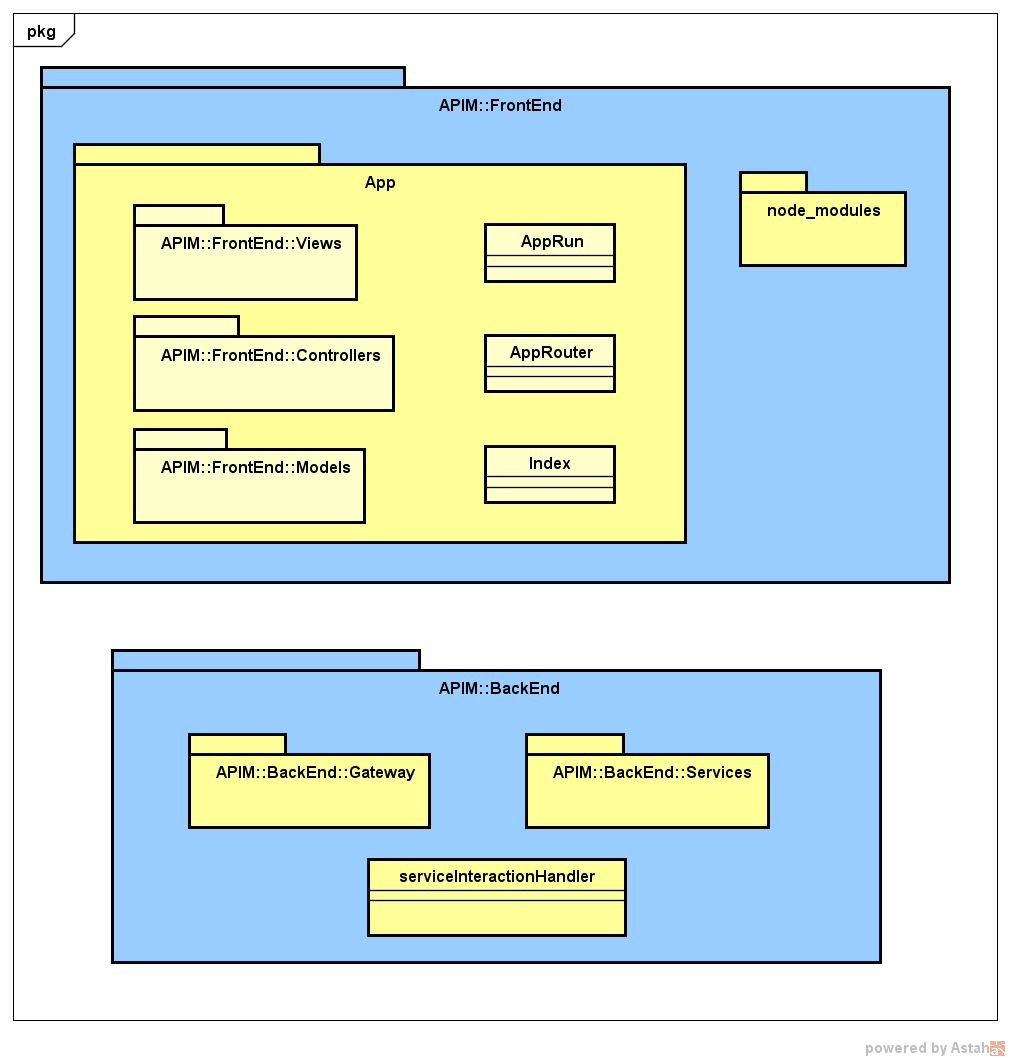
\includegraphics
	[width=0.7\linewidth]
	{images/APIM/Architettura_generale.png}
	\caption{Architettura generale}
\end{figure}

\subsubsection{Informazioni generali}
Di seguito, sono raccolte le informazioni generali dello schema presentato precedentemente:
	\begin{itemize}
		\item \textbf{Descrizione:} architettura ad alto livello della piattaforma \progetto.
		\item \textbf{Packages contenuti:}
		\begin{itemize}
			\item APIM::FrontEnd: package contenente tutti i packages che compongono la parte di front-end dell'applicazione;
			\item APIM::BackEnd: package contenente tutti i packages che compongono la parte di back-end dell'applicazione.
		\end{itemize}
	\end{itemize}

\newpage
\section{Specifica Front-End}

\subsection{APIM::FrontEnd}

\subsubsection{Informazioni generali}

\begin{figure}[H]
	\centering
	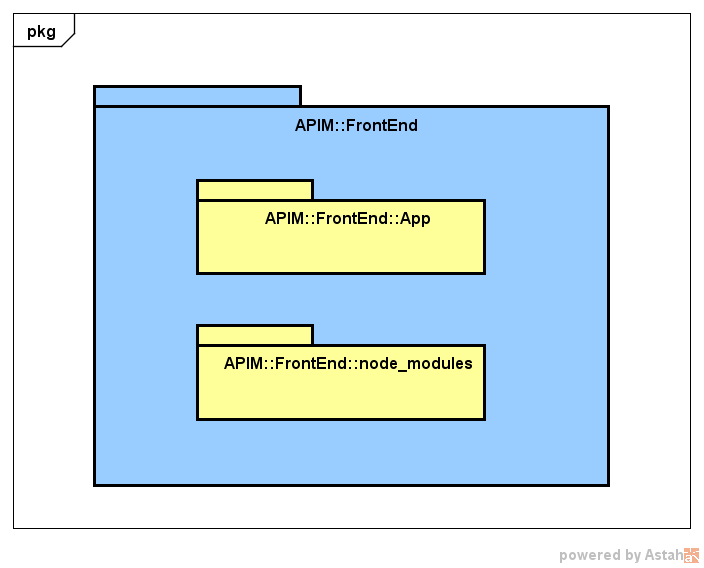
\includegraphics
	[width=0.7\linewidth]
	{images/APIM/FrontEnd/FrontEnd.png}
	\caption{APIM::FrontEnd}
\end{figure}

\begin{itemize}
	\item \textbf{Descrizione:} package contenente le componenti del lato front-end dell'applicazione web;
	\item \textbf{Packages contenuti:}
	\begin{itemize}
		\item App;
		\item node\_modules.
	\end{itemize}
\end{itemize}

\subsection{APIM::FrontEnd::App}

\subsubsection{Informazioni generali}

\begin{figure}[H]
	\centering
	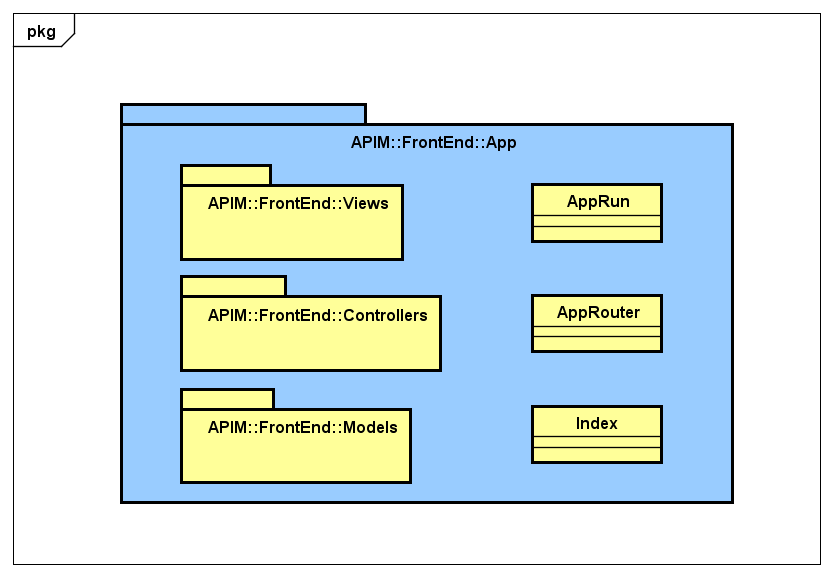
\includegraphics
	[width=0.7\linewidth]
	{images/APIM/FrontEnd/App.png}
	\caption{APIM::FrontEnd::App}
\end{figure}

\begin{itemize}
	\item \textbf{Descrizione:} Il package App contiene tutto il necessario al funzionamento del front-end dell'applicazione web API Market;
	\item \textbf{Packages contenuti:}
	\begin{itemize}
		\item Views;
		\item Models;
		\item Controllers.
	\end{itemize}
\end{itemize}

\subsubsection{Classi}

\paragraph{APIM::FrontEnd::App::AppRouter}

\begin{figure}[H]
	\centering
	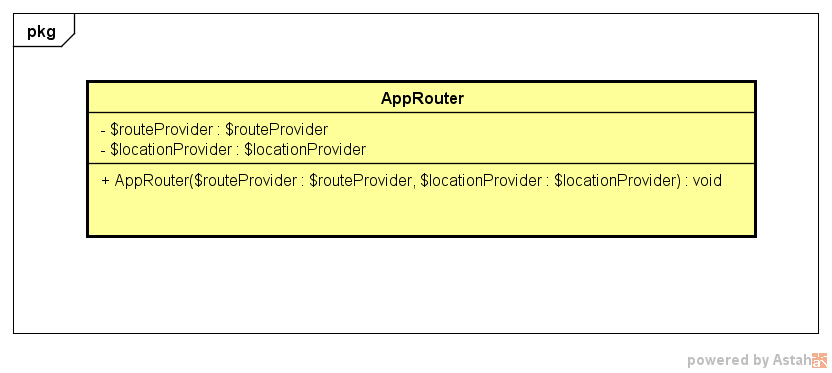
\includegraphics
	[width=0.7\linewidth]
	{images/APIM/FrontEnd/AppRouter.png}
	\caption{APIM::FrontEnd::App::AppRouter}
\end{figure}

\begin{itemize}
	\item \textbf{Descrizione:} La classe AppRouter gestisce le routes dell'applicazione, collegando le views con i rispettivi controllers attraverso i servizi di \$routeProvider e \$locationProvider;
	\item \textbf{Attributi:}
		\begin{itemize}
			\item \textbf{\$routeProvider:} \$routeProvider\\
			Campo dati con il riferimento al servizio di AngularJS dedicato al routing;
			\item \textbf{\$locationProvider:} \$locationProvider\\
			Campo dati con il riferimento al servizio di AngularJS dedicato al pathing;
		\end{itemize}
	\item \textbf{Metodi:}
		\begin{itemize}
			\item \textbf{AppRouter(\$routeProvider: \$routeProvider, \$locationProvider:
\$locationProvider):}
			Metodo per la gestione di routing e pathing dell'applicazione.
		\end{itemize}
\end{itemize}

\paragraph{APIM::FrontEnd::App::AppRun}

\begin{figure}[H]
	\centering
	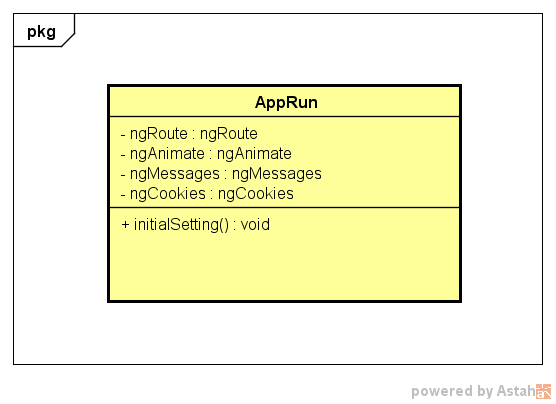
\includegraphics
	[width=0.7\linewidth]
	{images/APIM/FrontEnd/AppRun.png}
	\caption{APIM::FrontEnd::App::AppRun}
\end{figure}

\begin{itemize}
	\item \textbf{Descrizione:} La classe AppRun verifica la corretta autenticazione dell'utente e che le sue autorizzazioni gli consentano di visitare la pagina richiesta;
	\item \textbf{Attributi:}
		\begin{itemize}
			\item \textbf{ngRoute}: ngRoute\\
			Campo dati con il riferimento al modulo ngRoute di AngularJS;
			\item \textbf{ngAnimate}: ngAnimate\\
			Campo dati con il riferimento al modulo ngAnimate di AngularJS;
			\item \textbf{ngMessages}: ngMessages\\
			Campo dati con il riferimento al modulo ngMessages di AngularJS;
			\item \textbf{ngCookies}: ngCookies\\
			Campo dati con il riferimento al modulo ngCookies di AngularJS.
		\end{itemize}
	\item \textbf{Metodi:}
		\begin{itemize}
			\item \textbf{initialSetting(): void}
			Metodo per l'inizializzazione dei campi dati ai valori di default.
		\end{itemize}
	\item \textbf{Relazioni con altre classi:}
	\begin{itemize}
		\item Utilizza il modulo ngRoute per effettuare il routing dell'applicazione;
		\item Utilizza il modulo ngAnimate per impiegare transizioni ed animazioni nell'applicazione;
		\item Utilizza il modulo ngMessages per mostrare messaggi d'aiuto durante le procedure e form dell'applicazione;
		\item Utilizza il modulo ngCookies per effettuare il salvataggio dei cookies dell'applicazione.
	\end{itemize}
\end{itemize}

\paragraph{APIM::FrontEnd::App::Index}

\begin{figure}[H]
	\centering
	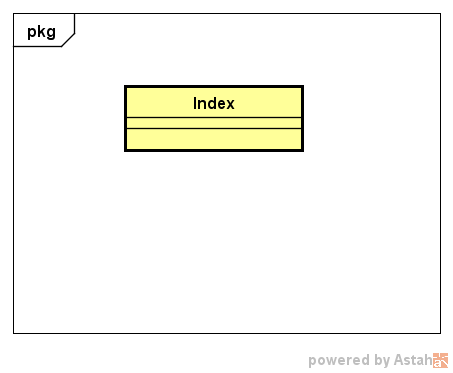
\includegraphics
	[width=0.7\linewidth]
	{images/APIM/FrontEnd/Index.png}
	\caption{APIM::FrontEnd::App::Index}
\end{figure}

\begin{itemize}
	\item \textbf{Descrizione:} La classe Index contiene la view principale dell'applicazione, dove l'utente visualizza dinamicamente le pagine che vuole visitare.
	\item \textbf{Relazioni con altre classi:}
	\begin{itemize}
		\item Interagisce con il package Views, necessario alla corretta visualizzazione delle pagine.
	\end{itemize}
\end{itemize}

% Fine App

\subsection{APIM::FrontEnd::App::Views}

\subsubsection{Informazioni generali}

\begin{figure}[H]
	\centering
	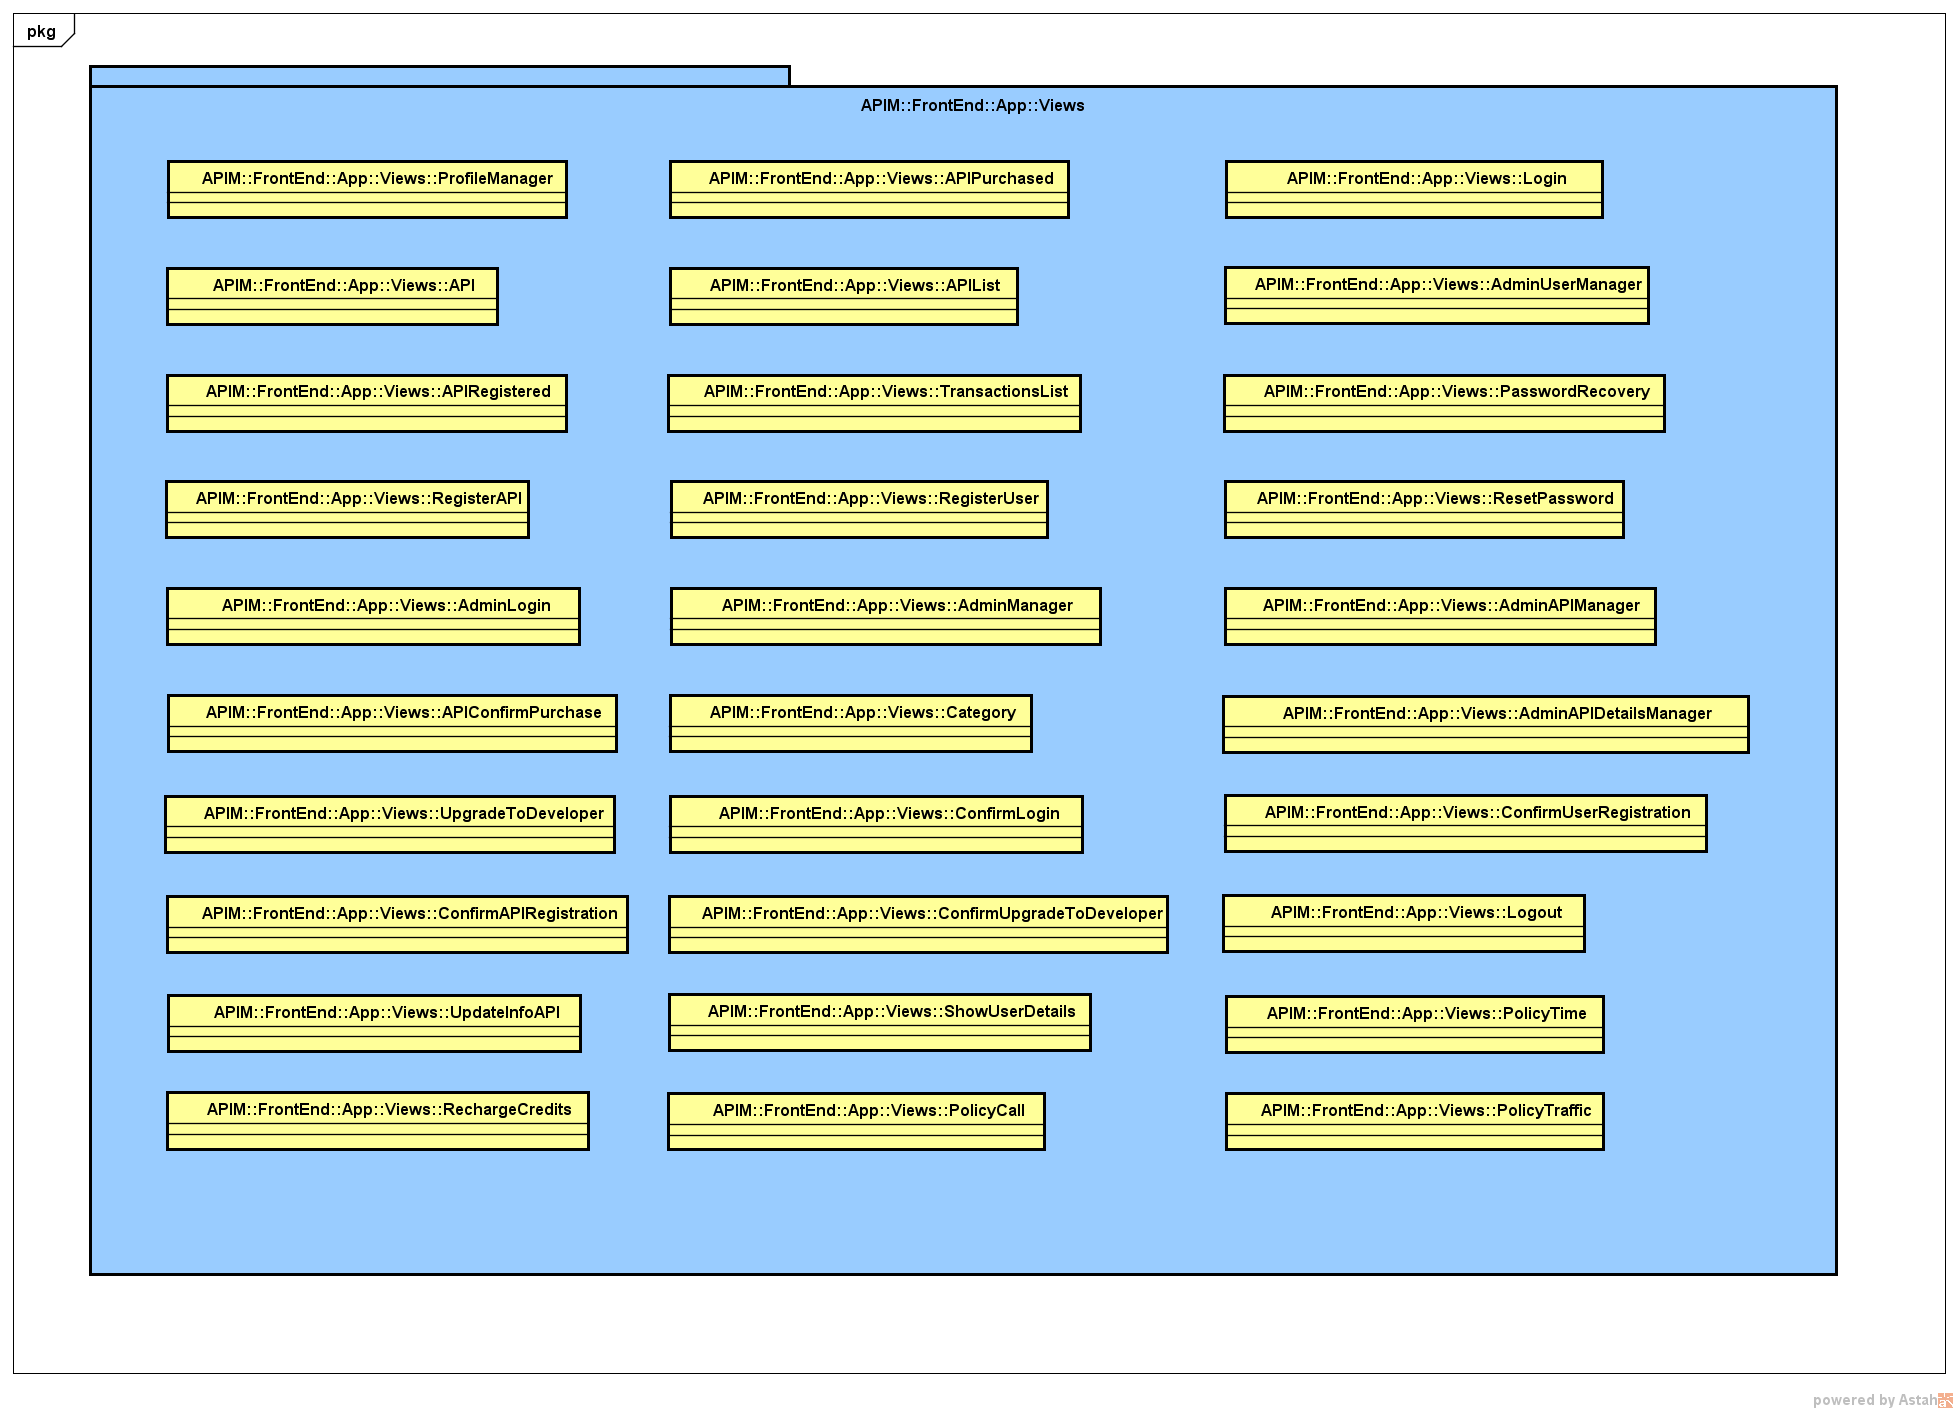
\includegraphics
	[width=0.7\linewidth]
	{images/APIM/FrontEnd/Views/views.png}
	\caption{APIM::FrontEnd::App::Views}
\end{figure}

\begin{itemize}
	\item \textbf{Descrizione:} Il package Views contiene tutte le view dell'applicazione.
	\item \textbf{Relazioni con altre classi:}
	\begin{itemize}
		\item Il package \textbf{Controllers} collega le views ad un controller per gestirne la visualizzazione da parte dell'utente; 
		\item Il package \textbf{Models} definisce le strutture dati utilizzate da views e controllers.
	\end{itemize}
\end{itemize}

\subsubsection{Classi}

\paragraph{APIM::FrontEnd::App::Views::ProfileManager}

\begin{figure}[H]
	\centering
	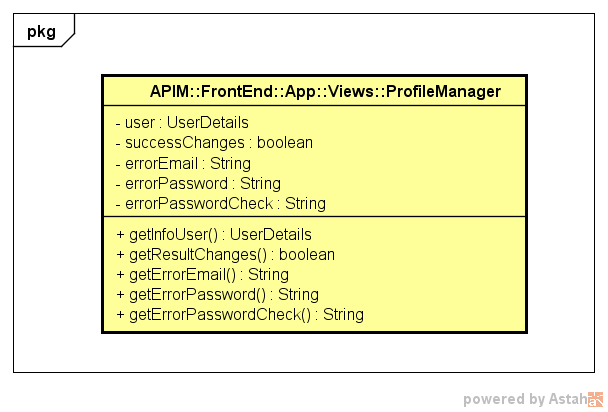
\includegraphics
	[width=0.7\linewidth]
	{images/APIM/FrontEnd/Views/ProfileManager.png}
	\caption{APIM::FrontEnd::App::Views::ProfileManager}
\end{figure}

\begin{itemize}
	\item \textbf{Descrizione:} View contenente il form dedicato alla registrazione di un utente,
il quale può inserire i campi necessari e registrarsi così alla piattaforma. Contiene,
inoltre, un link alla pagina di login;
	\item \textbf{Attributi:}
		\begin{itemize}
			\item \textbf{user : Object}\\
			Campo dati contenente le informazioni di un utente;
			\item \textbf{imageObject : Object}\\
			Campo dati contenente le informazioni dell'avatar dell'utente;
			\item \textbf{successChanges : string}\\
			Campo dati contenente la conferma delle modifiche;
			\item \textbf{errorEmail : string}\\
			Campo dati contenente l'eventuale errore di inserimento dell'email;
			\item \textbf{errorPassword : string}\\
			Campo dati contenente l'eventuale errore di inserimento della password;
			\item \textbf{errorPasswordCheck : string}\\
			Campo dati contenente l'eventuale errore della conferma della password.
		\end{itemize}
	\item \textbf{Relazioni con altre classi:}
	\begin{itemize}
		\item Interagisce con il controller \textbf{ProfileManagerController};
		\item Il model \textbf{UsersDetailModel} contiene le informazioni per rappresentare un utente.
	\end{itemize}
\end{itemize}

\paragraph{APIM::FrontEnd::App::Views::API}

\begin{figure}[H]
	\centering
	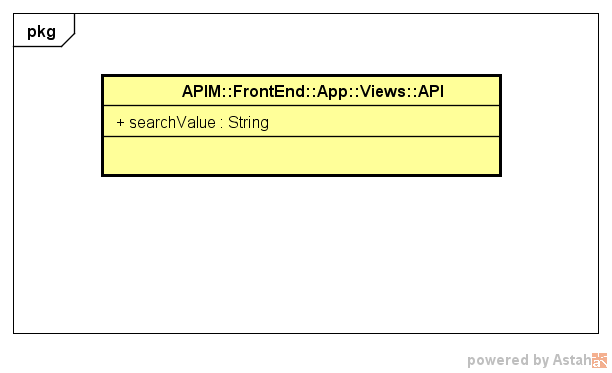
\includegraphics
	[width=0.7\linewidth]
	{images/APIM/FrontEnd/Views/API.png}
	\caption{APIM::FrontEnd::App::Views::API}
\end{figure}

\begin{itemize}
	\item \textbf{Descrizione:} View contenente i risultati della ricerca effettuata, che permette di selezionare un risultato presente al suo interno.
	\item \textbf{Attributi:}
		\begin{itemize}
			\item \textbf{searchValue : string}
			Campo dati contenente le keywords di ricerca dell'API.
		\end{itemize}
	\item \textbf{Relazioni con altre classi:}
	\begin{itemize}
		\item Interagisce con il controller \textbf{SearchController};
		\item Il model \textbf{MicroserviceModel} contiene le informazioni per rappresentare una API.
	\end{itemize}
\end{itemize}

\paragraph{APIM::FrontEnd::App::Views::APIRegistered}

\begin{figure}[H]
	\centering
	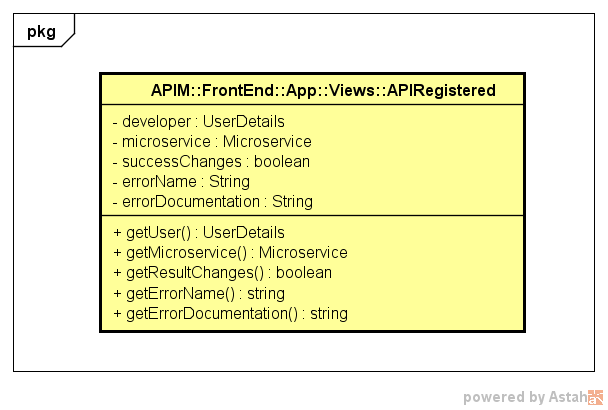
\includegraphics
	[width=0.7\linewidth]
	{images/APIM/FrontEnd/Views/APIRegistered.png}
	\caption{APIM::FrontEnd::App::Views::APIRegistered}
\end{figure}

\begin{itemize}
	\item \textbf{Descrizione:} View contenente la lista delle API registrate dall'utente sulla piattaforma.
	\item \textbf{Attributi:}
		\begin{itemize}
			\item \textbf{user : Object}\\
			Campo dati contenente le informazioni di un utente;
			\item \textbf{microservice : Object}\\
			Campo dati contenente le informazioni di un microservizio;
			\item \textbf{successChanges : string}\\
			Campo dati contenente la conferma delle modifiche;
			\item \textbf{errorName : string}\\
			Campo dati contenente l'eventuale errore di inserimento del nome;
			\item \textbf{errorDocumentation: string}\\
			Campo dati contenente l'eventuale errore di inserimento della documentazione.
		\end{itemize}
	\item \textbf{Relazioni con altre classi:}
	\begin{itemize}
		\item Interagisce con il controller \textbf{APIRegisteredController};
		\item Il model \textbf{UsersDetailModel} contiene le informazioni per rappresentare un utente;
		\item Il model \textbf{MicroserviceModel} contiene le informazioni per rappresentare una API.
	\end{itemize}
\end{itemize}

\paragraph{APIM::FrontEnd::App::Views::RegisterAPI}

\begin{figure}[H]
	\centering
	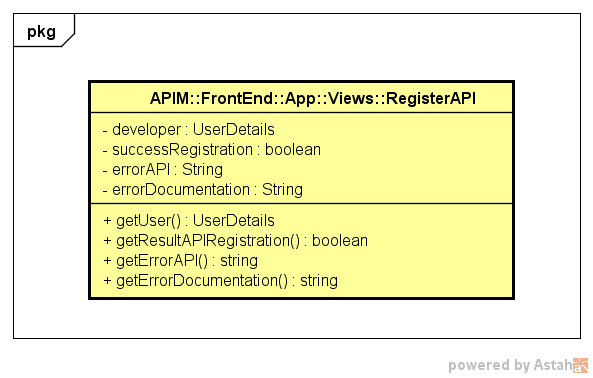
\includegraphics
	[width=0.7\linewidth]
	{images/APIM/FrontEnd/Views/RegisterAPI.png}
	\caption{APIM::FrontEnd::App::Views::RegisterAPI}
\end{figure}

\begin{itemize}
	\item \textbf{Descrizione:} View contenente il form per l'inserimento di una API da parte di un
utente sviluppatore. Lo sviluppatore può inserire tutti i dati relativi al microservizio
che intende esporre su API Market.
	\item \textbf{Attributi:}
		\begin{itemize}
			\item \textbf{user : Object}\\
			Campo dati contenente le informazioni di un utente;
			\item \textbf{microservice : Object}\\
			Campo dati contenente le informazioni di una API;
			\item \textbf{successRegistration : string}\\
			Campo dati contenente la conferma della registrazione;
			\item \textbf{errorAPI : string}\\
			Campo dati contenente l'eventuale errore di inserimento dell'API;
			\item \textbf{errorDocumentation: string}\\
			Campo dati contenente l'eventuale errore di inserimento della documentazione.
		\end{itemize}
	\item \textbf{Relazioni con altre classi:}
	\begin{itemize}
		\item Interagisce con il controller \textbf{APIRegistrationController};
		\item Il model \textbf{UsersDetailModel} contiene le informazioni per rappresentare un utente;
		\item Il model \textbf{MicroserviceModel} contiene le informazioni per rappresentare una API.
	\end{itemize}
\end{itemize}

\paragraph{APIM::FrontEnd::App::Views::SellingPolicy}

\begin{figure}[H]
	\centering
	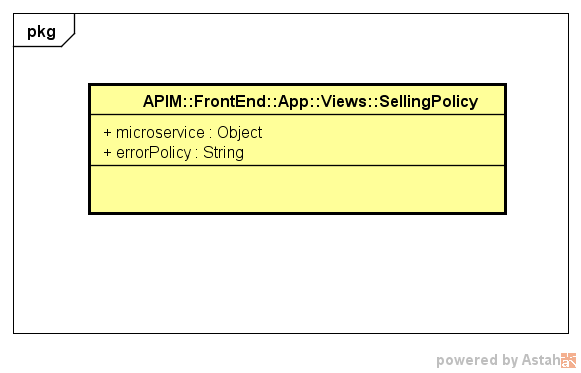
\includegraphics
	[width=0.7\linewidth]
	{images/APIM/FrontEnd/Views/SellingPolicy.png}
	\caption{APIM::FrontEnd::App::Views::SellingPolicy}
\end{figure}

\begin{itemize}
	\item \textbf{Descrizione:} View contenente il form per la gestione delle differenti policy di vendita
per un singolo microservizio.
	\item \textbf{Attributi:}
		\begin{itemize}
			\item \textbf{microservice : Object}\\
			Campo dati contenente le informazioni di una API;
			\item \textbf{errorPolicy : string}\\
			Campo dati contenente l'eventuale errore di inserimento della policy di vendita.
		\end{itemize}
	\item \textbf{Relazioni con altre classi:}
	\begin{itemize}
		\item Interagisce con il controller \textbf{SellingPolicyController};
		\item Il model \textbf{MicroserviceModel} contiene le informazioni per rappresentare una API.
	\end{itemize}
\end{itemize}

\paragraph{APIM::FrontEnd::App::Views::APIPurchased}

\begin{figure}[H]
	\centering
	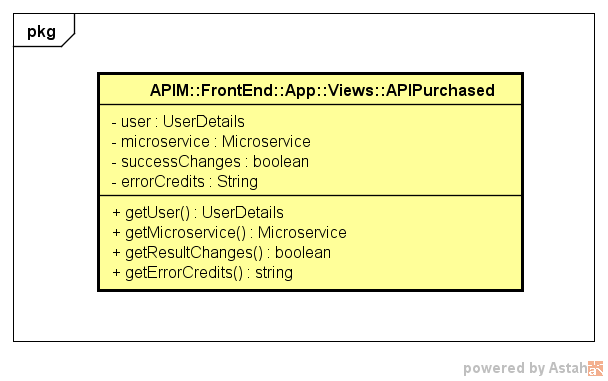
\includegraphics
	[width=0.7\linewidth]
	{images/APIM/FrontEnd/Views/APIPurchased.png}
	\caption{APIM::FrontEnd::App::Views::APIPurchased}
\end{figure}

\begin{itemize}
	\item \textbf{Descrizione:} View contenente la lista delle API acquistate da un utente della piattaforma API Market.
	\item \textbf{Attributi:}
		\begin{itemize}
			\item \textbf{user : Object}\\
			Campo dati contenente le informazioni di un utente;
			\item \textbf{microservice : Object}\\
			Campo dati contenente le informazioni di una API;
			\item \textbf{successChanges : string}\\
			Campo dati contenente la conferma del rinnovo dell'API;
			\item \textbf{errorCredits : string}\\
			Campo dati contenente l'eventuale errore di rinnovo dell'API.
		\end{itemize}
	\item \textbf{Relazioni con altre classi:}
	\begin{itemize}
		\item Interagisce con il controller \textbf{APIPurchasedController};
		\item Il model \textbf{UserDetailsModel} contiene le informazioni per rappresentare un utente;
		\item Il model \textbf{TransactionModel} contiene le informazioni per rappresentare una transazione;
		\item Il model \textbf{MicroserviceModel} contiene le informazioni per rappresentare una API.
	\end{itemize}
\end{itemize}

\paragraph{APIM::FrontEnd::App::Views::APIList}

\begin{figure}[H]
	\centering
	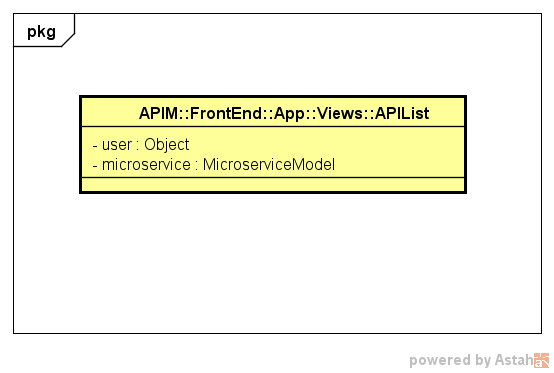
\includegraphics
	[width=0.7\linewidth]
	{images/APIM/FrontEnd/Views/APIList.png}
	\caption{APIM::FrontEnd::App::Views::APIList}
\end{figure}

\begin{itemize}
	\item \textbf{Descrizione:} View contenente la lista delle API in seguito ad una ricerca.
	\item \textbf{Attributi:}
	\begin{itemize}
		\item \textbf{user : Object}\\
		Campo dati contenente le informazioni di un utente;
		\item \textbf{microservice : Object}\\
		Campo dati contenente le informazioni di una API.
	\end{itemize}
	\item \textbf{Relazioni con altre classi:}
	\begin{itemize}
		\item Interagisce con il controller \textbf{APIListController};
		\item Il model \textbf{UserDetailsModel} contiene le informazioni per rappresentare un utente;
		\item Il model \textbf{MicroserviceModel} contiene le informazioni per rappresentare una API.
	\end{itemize}
\end{itemize}

\paragraph{APIM::FrontEnd::App::Views::TransactionsList}

\begin{figure}[H]
	\centering
	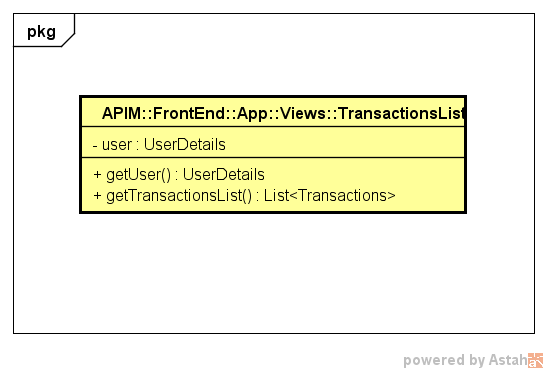
\includegraphics
	[width=0.7\linewidth]
	{images/APIM/FrontEnd/Views/TransactionsList.png}
	\caption{APIM::FrontEnd::App::Views::TransactionsList}
\end{figure}

\begin{itemize}
	\item \textbf{Descrizione:} View contenente l'elenco delle transazioni effettuate da un utente
su API Market.
	\item \textbf{Attributi:}
	\begin{itemize}
		\item \textbf{user : Object}\\
		Campo dati contenente le informazioni di un utente.
	\end{itemize}
	\item \textbf{Relazioni con altre classi:}
	\begin{itemize}
		\item Interagisce con il controller \textbf{TransactionsListController};
		\item Il model \textbf{TransactionModel} contiene le informazioni per rappresentare una API.
	\end{itemize}
\end{itemize}

\paragraph{APIM::FrontEnd::App::Views::RegisterUser}

\begin{figure}[H]
	\centering
	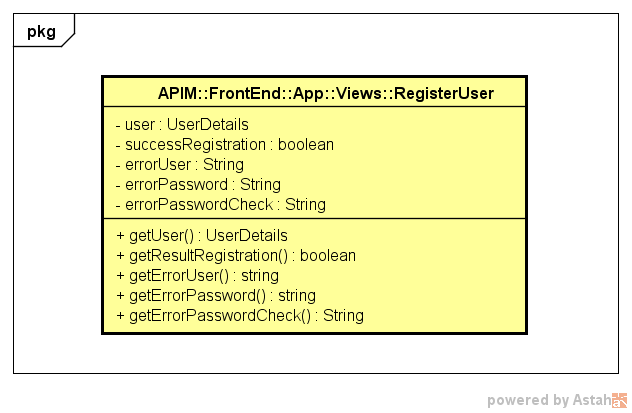
\includegraphics
	[width=0.7\linewidth]
	{images/APIM/FrontEnd/Views/RegisterUser.png}
	\caption{APIM::FrontEnd::App::Views::RegisterUser}
\end{figure}

\begin{itemize}
	\item \textbf{Descrizione:} View contenente il form dedicato alla registrazione di un utente, il
quale può inserire i campi necessari e registrarsi così alla piattaforma. Contiene,
inoltre, un link alla pagina di login;
	\item \textbf{Attributi:}
	\begin{itemize}
		\item \textbf{user : Object}\\
		Campo dati contenente le informazioni di un utente;
		\item \textbf{successRegistration : string}\\
		Campo dati contenente il messaggio di successo della registrazione;
		\item \textbf{errorUser : string}\\
		Campo dati contenente l'eventuale errore di inserimento delle informazioni dell'utente;
		\item \textbf{errorPassword : string}\\
		Campo dati contenente l'eventuale errore di inserimento della password;
		\item \textbf{errorPasswordCheck : string}\\
		Campo dati contenente l'eventuale errore di reinserimento della password.
	\end{itemize}
	\item \textbf{Relazioni con altre classi:}
	\begin{itemize}
		\item Interagisce con il controller \textbf{RegisterUserController};
		\item Il model \textbf{UserDetailsModel} contiene le informazioni per rappresentare un utente.
	\end{itemize}
\end{itemize}

\paragraph{APIM::FrontEnd::App::Views::AdminManager}

\begin{figure}[H]
	\centering
	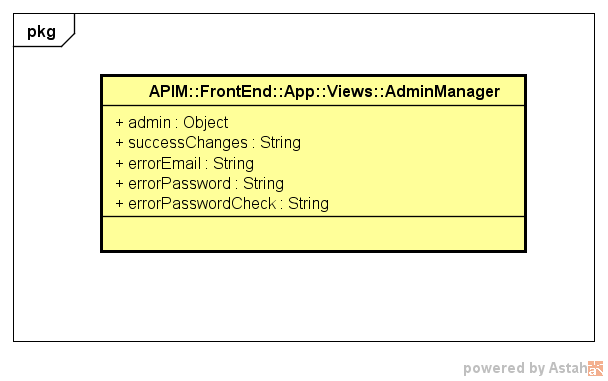
\includegraphics
	[width=0.7\linewidth]
	{images/APIM/FrontEnd/Views/AdminManager.png}
	\caption{APIM::FrontEnd::App::Views::AdminManager}
\end{figure}

\begin{itemize}
	\item \textbf{Descrizione:} View contenente le operazioni per la gestione del profilo amministratore
API Market.
	\item \textbf{Attributi:}
	\begin{itemize}
		\item \textbf{user : Object}\\
		Campo dati contenente le informazioni di un utente;
		\item \textbf{successChanges : string}\\
		Campo dati contenente il messaggio di successo delle modifiche;
		\item \textbf{errorUser : string}\\
		Campo dati contenente l'eventuale errore di inserimento delle informazioni dell'utente;
		\item \textbf{errorPassword : string}\\
		Campo dati contenente l'eventuale errore di inserimento della password;
		\item \textbf{errorPasswordCheck : string}\\
		Campo dati contenente l'eventuale errore di reinserimento della password.
	\end{itemize}
	\item \textbf{Relazioni con altre classi:}
	\begin{itemize}
		\item Interagisce con il controller \textbf{AdminManagerController};
		\item Il model \textbf{UserDetailsModel} contiene le informazioni per rappresentare un utente.
	\end{itemize}
\end{itemize}

\paragraph{APIM::FrontEnd::App::Views::Login}

\begin{figure}[H]
	\centering
	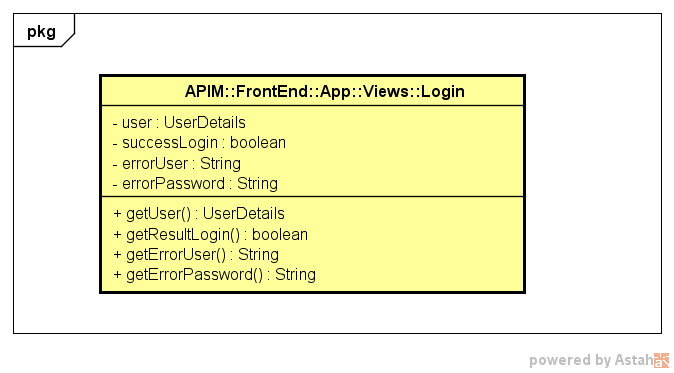
\includegraphics
	[width=0.7\linewidth]
	{images/APIM/FrontEnd/Views/Login.png}
	\caption{APIM::FrontEnd::App::Views::Login}
\end{figure}

\begin{itemize}
	\item \textbf{Descrizione:} View contenente il form necessario affinchè l'utente possa effettuare il login ed autenticarsi al sistema. Contiene, inoltre, un link alla pagina di registrazione e uno alla pagina per il recupero della password
	\item \textbf{Attributi:}
	\begin{itemize}
		\item \textbf{user : Object}\\
		Campo dati contenente le informazioni di un utente;
		\item \textbf{successLogin : string}\\
		Campo dati contenente il messaggio di successo del login;
		\item \textbf{errorUser : string}\\
		Campo dati contenente l'eventuale errore di inserimento delle informazioni dell'utente;
		\item \textbf{errorPassword : string}\\
		Campo dati contenente l'eventuale errore di inserimento della password.
	\end{itemize}
	\item \textbf{Relazioni con altre classi:}
	\begin{itemize}
		\item Interagisce con il controller \textbf{LoginController};
		\item Il model \textbf{UserDetailsModel} contiene le informazioni per rappresentare un utente.
	\end{itemize}
\end{itemize}

\paragraph{APIM::FrontEnd::App::Views::VirtualAccount}

\begin{figure}[H]
	\centering
	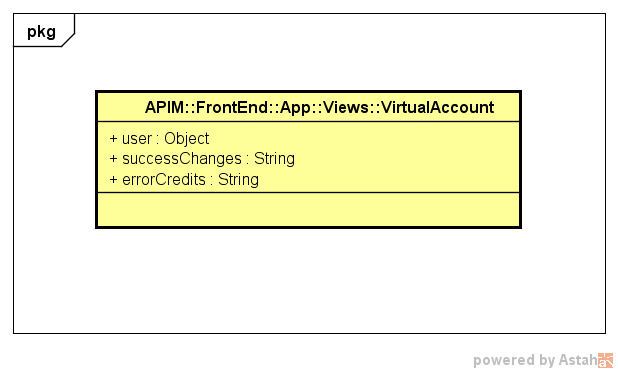
\includegraphics
	[width=0.7\linewidth]
	{images/APIM/FrontEnd/Views/VirtualAccount.png}
	\caption{APIM::FrontEnd::App::Views::VirtualAccount}
\end{figure}

\begin{itemize}
	\item \textbf{Descrizione:} View contenente le informazioni relative al conto virtuale personale
associato al profilo utente.
	\item \textbf{Attributi:}
	\begin{itemize}
		\item \textbf{user : Object}\\
		Campo dati contenente le informazioni di un utente;
		\item \textbf{successChanges : string}\\
		Campo dati contenente il messaggio di successo della ricarica crediti;
		\item \textbf{errorCredits : string}\\
		Campo dati contenente l'eventuale errore di acquisto crediti.
	\end{itemize}
	\item \textbf{Relazioni con altre classi:}
	\begin{itemize}
		\item Interagisce con il controller \textbf{VirtualAccountController};
		\item Il model \textbf{UserDetailsModel} contiene le informazioni per rappresentare un utente;
		\item Il model \textbf{TransactionModel} contiene le informazioni per rappresentare una transazione.
	\end{itemize}
\end{itemize}

\paragraph{APIM::FrontEnd::App::Views::PasswordRecovery}

\begin{figure}[H]
	\centering
	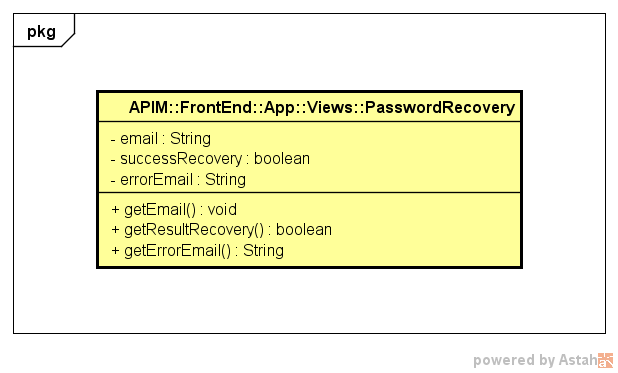
\includegraphics
	[width=0.7\linewidth]
	{images/APIM/FrontEnd/Views/PasswordRecovery.png}
	\caption{APIM::FrontEnd::App::Views::PasswordRecovery}
\end{figure}

\begin{itemize}
	\item \textbf{Descrizione:} View contenente il form dedicato al recupero della password di un utente, il quale può inserire l'indirizzo email e ricevere una nuova password con la quale autenticarsi al sistema. Contiene, inoltre, un link alla pagina di login;
	\item \textbf{Attributi:}
	\begin{itemize}
		\item \textbf{email : string}\\
		Campo dati contenente un indirizzo email;
		\item \textbf{successRecovery : string}\\
		Campo dati contenente il messaggio di successo del recupero password;
		\item \textbf{errorEmail : string}\\
		Campo dati contenente l'eventuale errore di inserimento dell'indirizzo email.
	\end{itemize}
	\item \textbf{Relazioni con altre classi:}
	\begin{itemize}
		\item Interagisce con il controller \textbf{PasswordRecoveryController};
		\item Il model \textbf{UserDetailsModel} contiene le informazioni per rappresentare un utente.
	\end{itemize}
\end{itemize}

\paragraph{APIM::FrontEnd::App::Views::ResetPassword}

\begin{figure}[H]
	\centering
	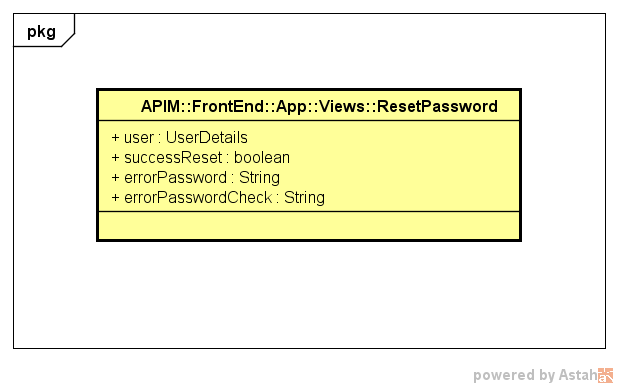
\includegraphics
	[width=0.7\linewidth]
	{images/APIM/FrontEnd/Views/ResetPassword.png}
	\caption{APIM::FrontEnd::App::Views::ResetPassword}
\end{figure}

\begin{itemize}
	\item \textbf{Descrizione:} View contenente il form dedicato al cambio di password di un utente
autenticato, il quale può inserire la nuova password che intende utilizzare per i futuri login al sistema.
	\item \textbf{Attributi:}
	\begin{itemize}
		\item \textbf{user : Object}\\
		Campo dati contenente le informazioni di un utente;
		\item \textbf{successReset : string}\\
		Campo dati contenente il messaggio di successo del reset password;
		\item \textbf{errorPassword : string}\\
		Campo dati contenente l'eventuale errore di inserimento della password.
		\item \textbf{errorPasswordCheck : string}\\
		Campo dati contenente l'eventuale errore di reinserimento della password.
	\end{itemize}
	\item \textbf{Relazioni con altre classi:}
	\begin{itemize}
		\item Interagisce con il controller \textbf{ResetPasswordController};
		\item Il model \textbf{UserDetailsModel} contiene le informazioni per rappresentare un utente.
	\end{itemize}
\end{itemize}

\paragraph{APIM::FrontEnd::App::Views::AdminModeration}

\begin{figure}[H]
	\centering
	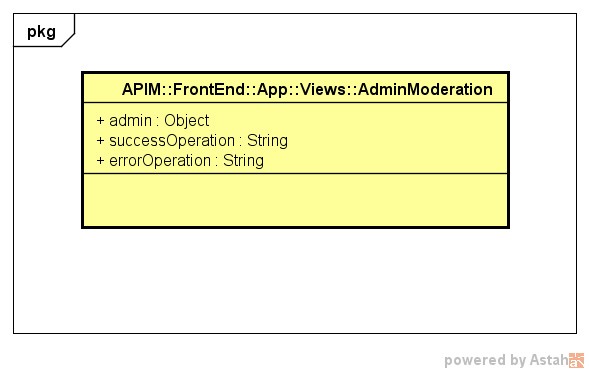
\includegraphics
	[width=0.7\linewidth]
	{images/APIM/FrontEnd/Views/AdminModeration.png}
	\caption{APIM::FrontEnd::App::Views::AdminModeration}
\end{figure}

\begin{itemize}
	\item \textbf{Descrizione:} View contenente il form dedicato alla moderazione di un utente o di una API da parte di un amministratore della piattaforma API Market.
	\item \textbf{Attributi:}
	\begin{itemize}
		\item \textbf{admin : Object}\\
		Campo dati contenente le informazioni di un utente;
		\item \textbf{successOperation : string}\\
		Campo dati contenente il messaggio di successo dell'operazione di moderazione;
		\item \textbf{errorOperation : string}\\
		Campo dati contenente l'eventuale errore dell'operazione di moderazione.
	\end{itemize}
	\item \textbf{Relazioni con altre classi:}
	\begin{itemize}
		\item Interagisce con il controller \textbf{AdminModerationController};
		\item Il model \textbf{UserDetailsModel} contiene le informazioni per rappresentare un utente.
	\end{itemize}
\end{itemize}


%Fine views

\subsection{APIM::FrontEnd::App::Models}

\subsubsection{Informazioni generali}

\begin{figure}[H]
	\centering
	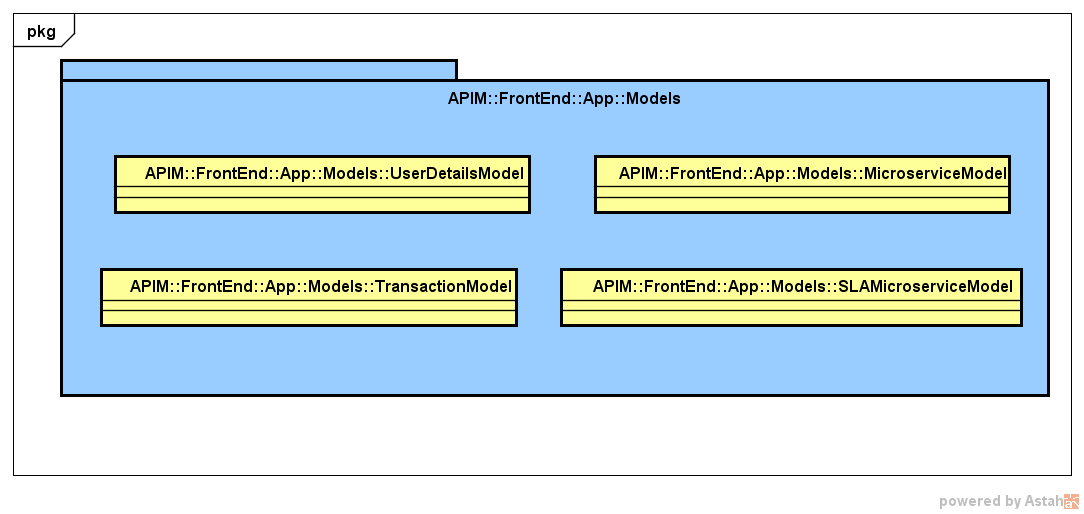
\includegraphics
	[width=0.7\linewidth]
	{images/APIM/FrontEnd/Models/Models.png}
	\caption{APIM::FrontEnd:App:Models}
\end{figure}

\begin{itemize}
	\item \textbf{Descrizione:} Il package Models contiene le classi che definiscono le strutture dei dati di utenti, microservizi, transazioni e sondaggi SLA.
	\item \textbf{Relazioni con altre classi:}
		\begin{itemize}
			\item Interagisce con i package \textbf{Controllers} e \textbf{Views} per garantire il dynamic binding di AngularJS.
		\end{itemize}
\end{itemize}

\subsubsection{Classi}

\paragraph{APIM::FrontEnd::App::Models::UserDetailsModel}

\begin{figure}[H]
	\centering
	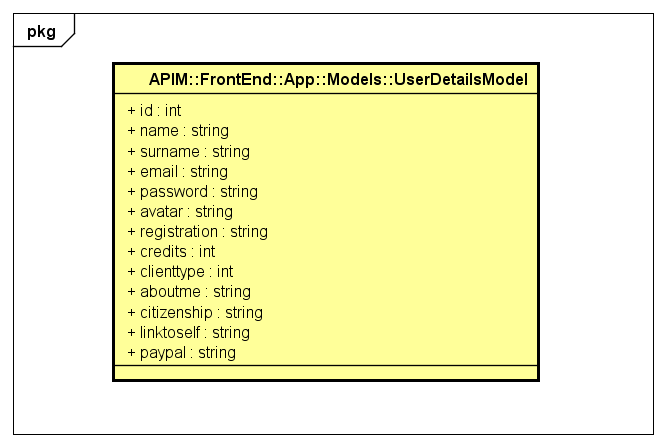
\includegraphics
	[width=0.7\linewidth]
	{images/APIM/FrontEnd/Models/UserDetailsModel.png}
	\caption{APIM::FrontEnd::App::Models:UserDetailsModel}
\end{figure}

\begin{itemize}
	\item \textbf{Descrizione:} UserDetailsModel che rappresenta un utente e che contiene tutte le informazioni
necessarie alla presentazione del contenuto di un utente, sia nella visualizzazione che nella gestione di un profilo.
	\item \textbf{Attributi:}
		\begin{itemize}
			\item \textbf{id : int}\\
			Id dell'utente;
			\item \textbf{name : string}\\
			Nome dell'utente;
			\item \textbf{surname : string}\\
			Cognome dell'utente;
			\item \textbf{email : string}\\
			Email dell'utente;
			\item \textbf{password : string}\\
			Password dell'utente;
			\item \textbf{avatar : string}\\
			Avatar dell'utente;
			\item \textbf{registration : string}\\
			Data di registrazione dell'utente;
			\item \textbf{credits : int}\\
			Crediti dell'utente;
			\item \textbf{clienttype : int}\\
			Tipo di account dell'utente;
			\item \textbf{aboutme : string}\\
			AboutMe dell'utente sviluppatore;
			\item \textbf{citizenship : string}\\
			Cittadinanza dell'utente sviluppatore;
			\item \textbf{linktoself : string}\\
			Link al sito esterno dell'utente sviluppatore;
			\item \textbf{paypal : string}\\
			Email paypal dell'utente sviluppatore.
		\end{itemize}
	\item \textbf{Relazioni con altre classi:}
		\begin{itemize}
			\item Interagisce con il controller \textbf{LoginController};
			\item Interagisce con il controller \textbf{SearchController};
			\item Interagisce con il controller \textbf{ProfileManagerController};
			\item Interagisce con il controller \textbf{ResetPasswordController};
			\item Interagisce con il controller \textbf{PasswordRecoveryController};
			\item Interagisce con il controller \textbf{Controller};
			\item Interagisce con il controller \textbf{VirtualAccountController}.
	\end{itemize}
\end{itemize}

\paragraph{APIM::FrontEnd::App::Models::TransactionModel}

\begin{figure}[H]
	\centering
	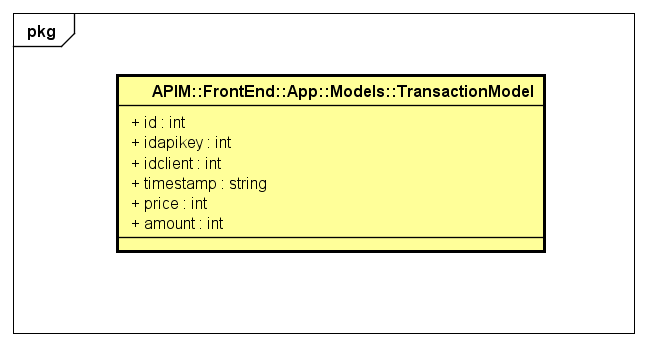
\includegraphics
	[width=0.7\linewidth]
	{images/APIM/FrontEnd/Models/TransactionModel.png}
	\caption{APIM::FrontEnd::App::Models::TransactionModel}
\end{figure}

\begin{itemize}
	\item \textbf{Descrizione:} TransactionModel rappresenta una transazione avvenuta e che contiene
tutte le informazioni necessarie alla presentazione del contenuto di una transazione,
sia nella visualizzazione che nella gestione.
	\item \textbf{Attributi:}
		\begin{itemize}
			\item \textbf{id : int}\\
			Id della transazione;
			\item \textbf{idapikey : int}\\
			Id dell'apikey;
			\item \textbf{idclient : int}\\
			Id del cliente;
			\item \textbf{timestamp : int}\\
			Data ed ora della transazione;
			\item \textbf{price : int}\\
			Prezzo della transazione;
			\item \textbf{amount : int}\\
			Ammontare quantitativo della transazione.
		\end{itemize}
	\item \textbf{Relazioni con altre classi:}
		\begin{itemize}
			\item Interagisce con il controller \textbf{TransactionsListController};
			\item Interagisce con il controller \textbf{APIPurchasedController}.
		\end{itemize}
\end{itemize}

\paragraph{APIM::FrontEnd::App::Models::MicroserviceModel}

\begin{figure}[H]
	\centering
	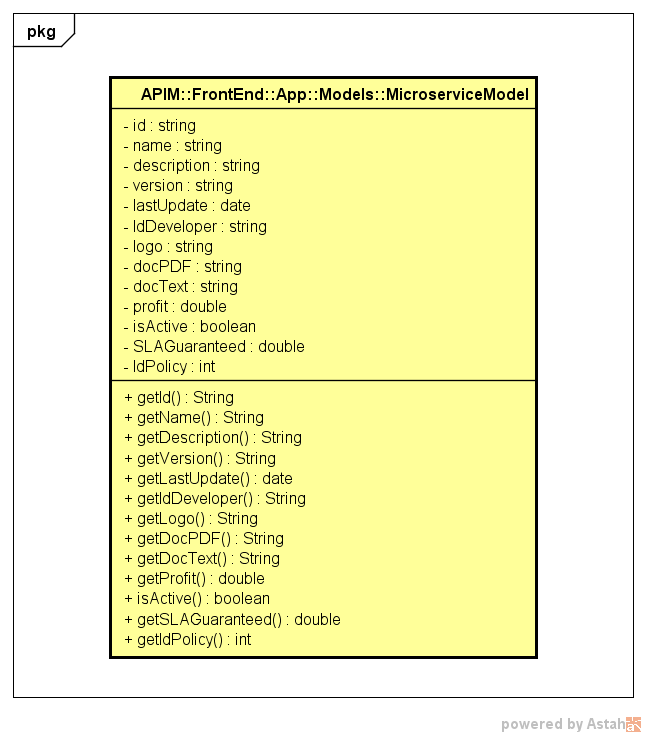
\includegraphics
	[width=0.7\linewidth]
	{images/APIM/FrontEnd/Models/MicroserviceModel.png}
	\caption{APIMarket::FrontEnd::App::Models::MicroserviceModel}
\end{figure}

\begin{itemize}
	\item \textbf{Descrizione:} MicroserviceModel rappresenta un microservizio e che contiene tutte le
informazioni necessarie alla presentazione del contenuto di un microservizio, sia nella visualizzazione che nella gestione.
	\item \textbf{Attributi:}
		\begin{itemize}
			\item \textbf{id : int}\\
			Id del microservizio;
			\item \textbf{name : string}\\
			Nome del microservizio;
			\item \textbf{description : string}\\
			Descrizione del microservizio;
			\item \textbf{version : string}\\
			Versione corrente del microservizio;
			\item \textbf{lastupdate : string}\\
			Data ultimo aggiornamento del microservizio;
			\item \textbf{iddeveloper : string}\\
			Id dello sviluppatore del microservizio;
			\item \textbf{logo : string}\\
			Link al logo del microservizio;
			\item \textbf{docpdf : string}\\
			Link al file PDF del microservizio;
			\item \textbf{docext : string}\\
			Link alla documentazione esterna del microservizio;
			\item \textbf{profit : int}\\
			Percentuale profitto dello sviluppatore del microservizio;
			\item \textbf{isactive : bool}\\
			Funzionamento attuale del microservizio;
			\item \textbf{slaguaranteed : double}\\
			SLA garantita dal microservizio;
			\item \textbf{idpolicy : int}\\
			Id della policy di vendita del microservizio.
		\end{itemize}
	\item \textbf{Relazioni con altre classi:}
		\begin{itemize}
			\item Interagisce con il controller \textbf{APIRegiteredController};
			\item Interagisce con il controller \textbf{APIRegistrationController};
			\item Interagisce con il controller \textbf{SellingPolicyController};
			\item Interagisce con il controller \textbf{APIPurchasedController};
			\item Interagisce con il controller \textbf{APIListController}.
		\end{itemize}
\end{itemize}

\paragraph{APIM::FrontEnd::App::Models::SLAMicroserviceModel}

\begin{figure}[H]
	\centering
	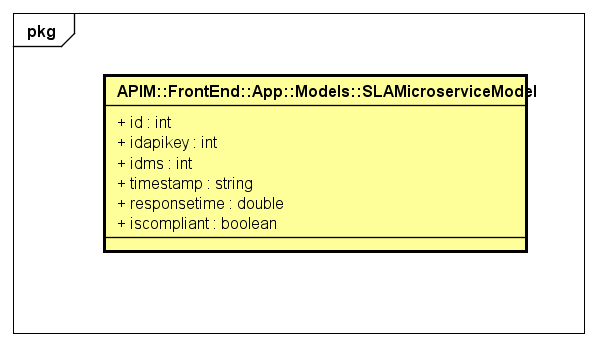
\includegraphics
	[width=0.7\linewidth]
	{images/APIM/FrontEnd/Models/SLAMicroserviceModel.png}
	\caption{APIM::FrontEnd::App::Models::SLAMicroserviceModel}
\end{figure}

\begin{itemize}
	\item \textbf{Descrizione:} SLAMicroserviceModel rappresenta la SLA di un microservizio e che
contiene tutte le informazioni necessarie alla presentazione del contenuto di SLA di un microservizio, sia nella visualizzazione che nella gestione.
	\item \textbf{Attributi:}
		\begin{itemize}
			\item \textbf{id : int}\\
			Id del sondaggio SLA;
			\item \textbf{idapikey : int}\\
			Id dell'apike attribuita al sondaggio SLA;
			\item \textbf{idms : int}\\
			Id del microservizio attribuito al sondaggio SLA;
			\item \textbf{timestamp : string}\\
			Data ed ora del sondaggio SLA;
			\item \textbf{responsetime : int}\\
			Tempo di risposta del sondaggio SLA;
			\item \textbf{iscompliant : boolean}\\
			Indicatore del rispetto del sondaggio SLA.
		\end{itemize}
	\item \textbf{Relazioni con altre classi:}
		\begin{itemize}
			\item Interagisce con il controller \textbf{SellingPolicyController};
			\item Interagisce con il controller \textbf{APIRegistrationController}.		
		\end{itemize}
\end{itemize}

%Fine models

\subsection{APIM::FrontEnd::App::Controllers}

\subsubsection{Informazioni generali}

\begin{figure}[H]
	\centering
	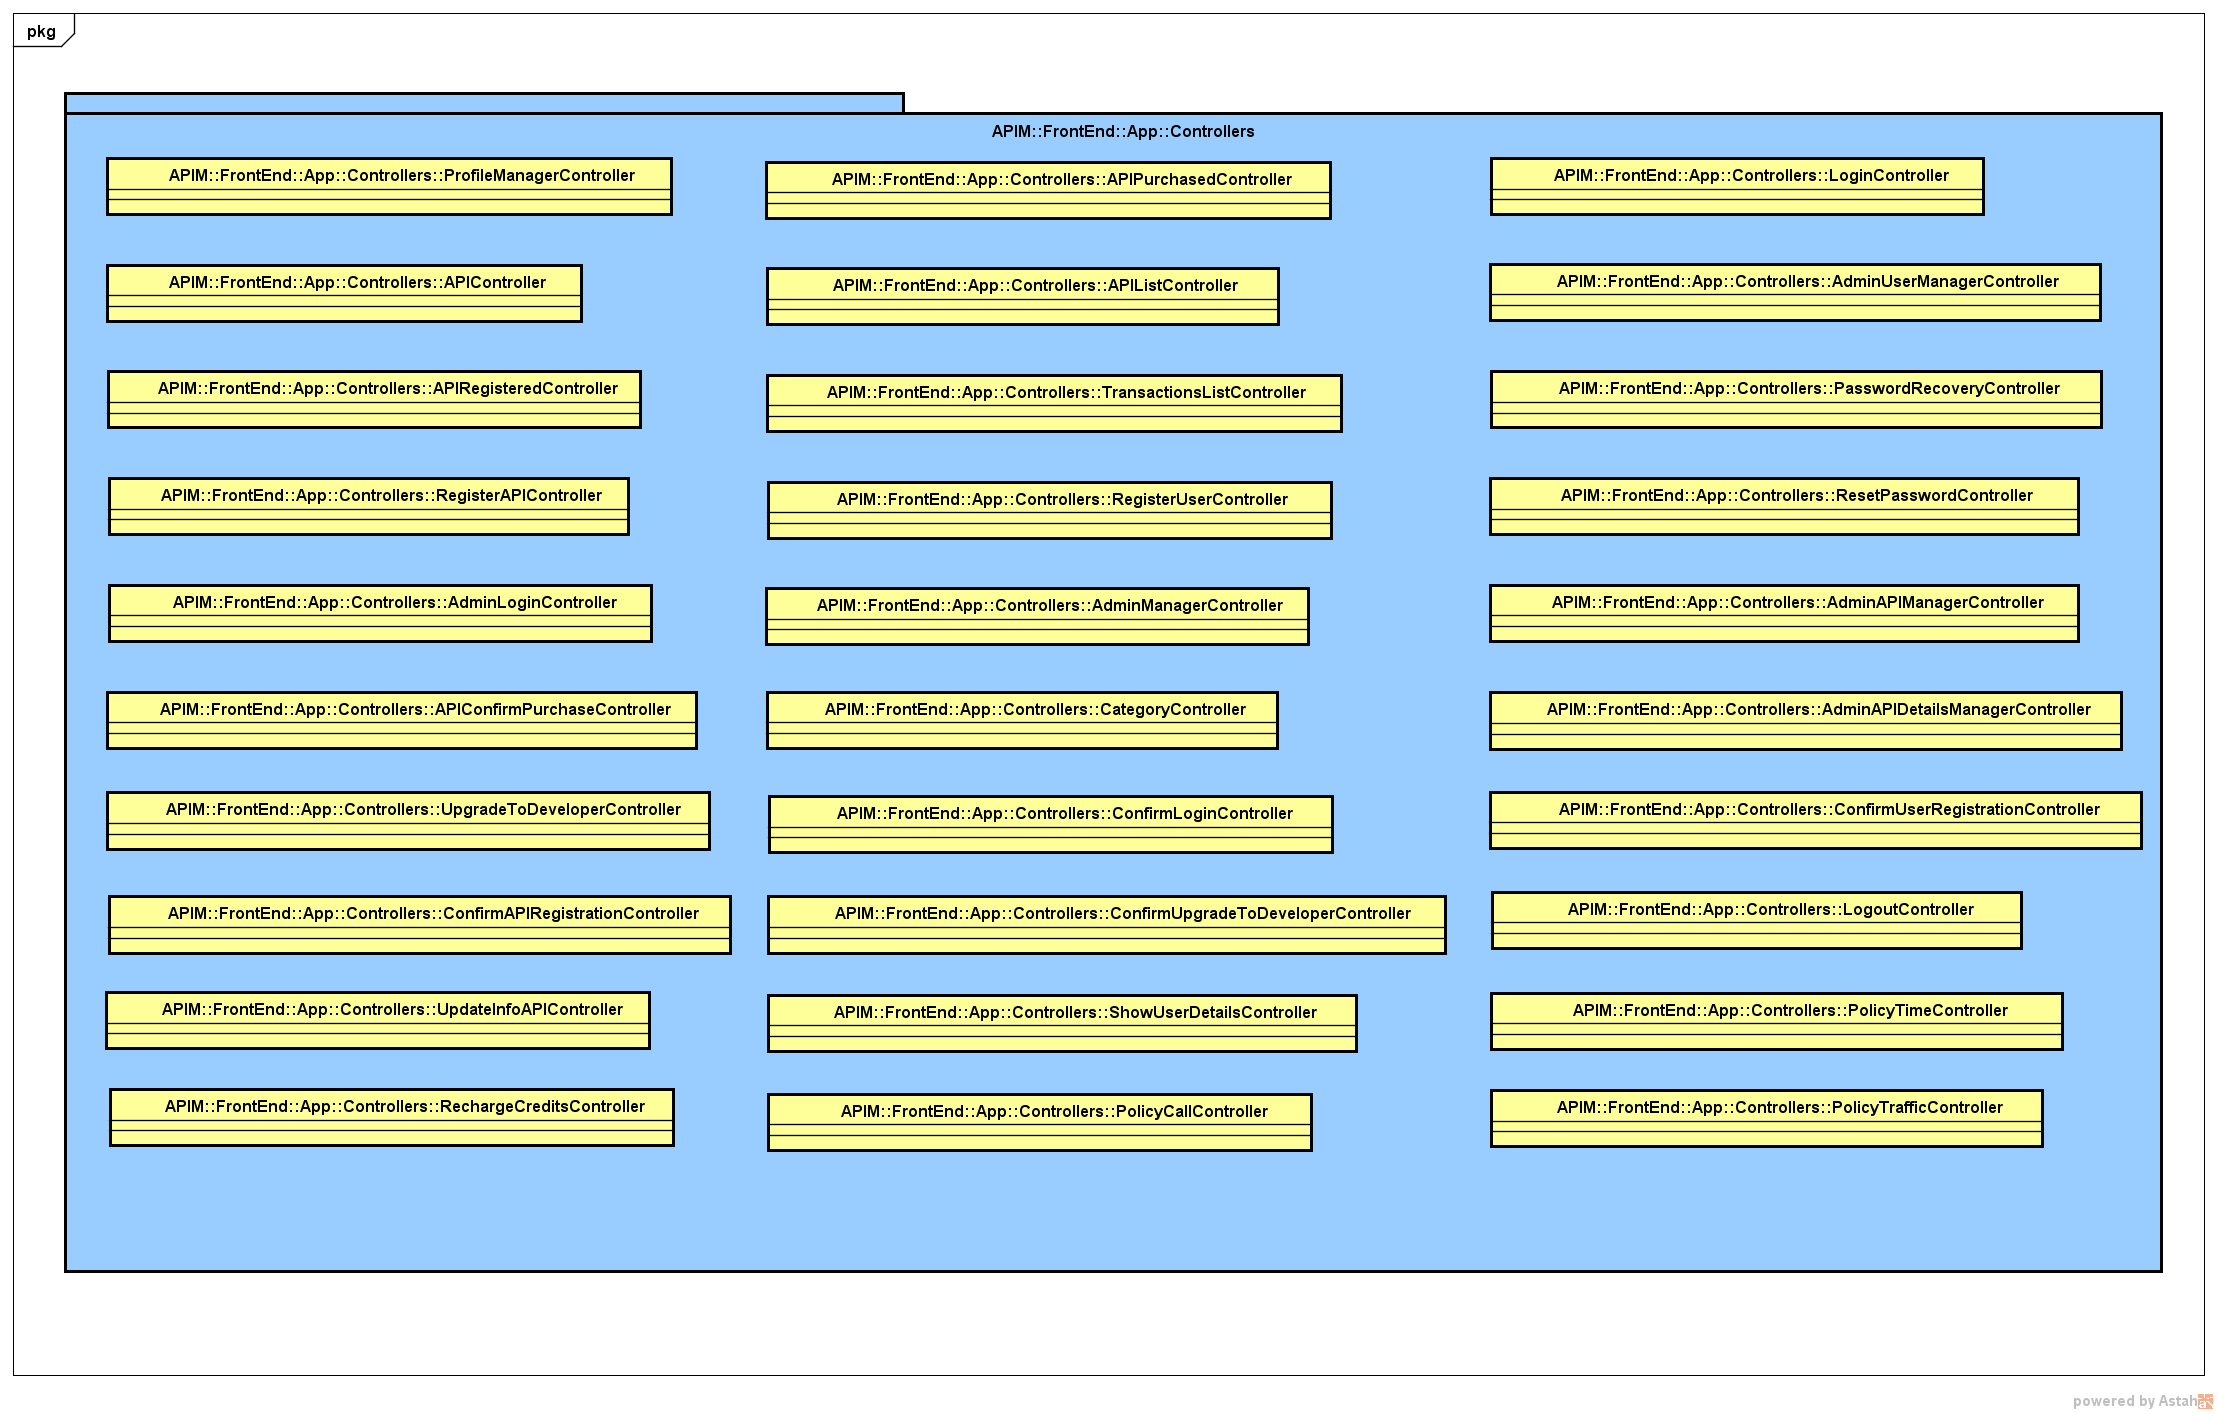
\includegraphics
	[width=0.7\linewidth]
	{images/APIM/FrontEnd/Controllers/Controllers.png}
	\caption{APIM::FrontEnd::App::Controllers}
\end{figure}

\begin{itemize}
	\item \textbf{Descrizione:} Il package Controllers contiene tutti i controller dell'applicazione.
	\item \textbf{Relazioni con altre classi:}
		\begin{itemize}
			\item Il package \textbf{View} è collegato ad un controller per gestirne la visualizzazione delle pagine ed il routing; 
			\item Il package \textbf{Models} contiene le strutture dati cui i controllers si riferiscono.
		\end{itemize}
\end{itemize}

\subsubsection{Classi}

\paragraph{APIM::FrontEnd::App::Controllers::ProfileManagerController}

\begin{figure}[H]
	\centering
	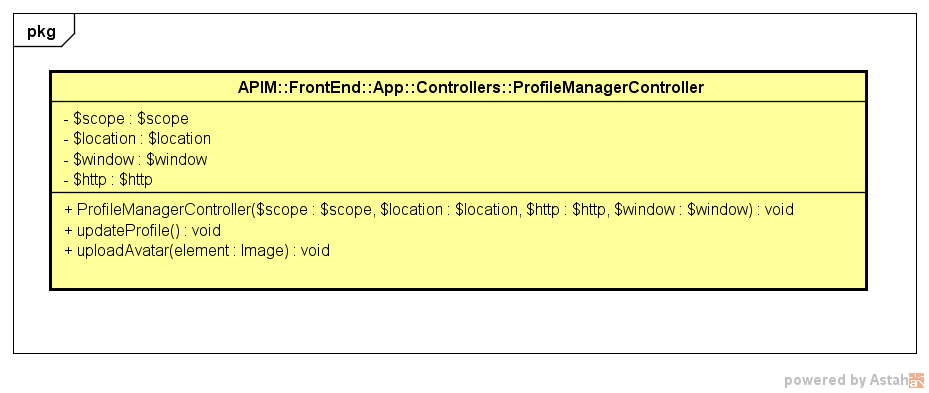
\includegraphics
	[width=0.7\linewidth]
	{images/APIM/FrontEnd/Controllers/ProfileManagerController.png}
	\caption{APIM::FrontEnd::App::Controllers::ProfileManagerController}
\end{figure}

\begin{itemize}
	\item \textbf{Descrizione:} ProfileManagerController permette di gestire il profilo personale di un
utente, fornendo le funzionalità all'utente per poter modificare i propri dati.
	\item \textbf{Attributi:}
		\begin{itemize}
		
			\item \textbf{\$scope : \$scope}\\
			Campo dati contenente un riferimento all'oggetto \$scope creato da AngularJS, viene utilizzato come mezzo di comunicazione tra il controller e la view. Contiene gli oggetti che definiscono il model dell'applicazione;
			
			\item \textbf{\$rootScope : \$rootScope}\\
			Campo dati contenente il riferimento all'oggetto globale \$rootScope creato da AngularJS. Viene utilizzato per rendere accessibile a tutti i controllers e a tutte le views l'oggetto UserDetailsModel;
				
			\item \textbf{\$timeout : \$timeout }\\
			Campo dati contenente il riferimento all'oggetto globale \$timeout creato da AngularJS. Il valore di ritorno di una chiamata alla funzione di \$timeout è una promise, la quale
sarà risolta quando avverrà il ritardo e la funzione di timeout eseguita;

			\item \textbf{\$http : \$http }\\
			Campo dati che contiene un riferimento al servizio \$http che permette la comunicazione con il protocollo HTTP;
				
			\item \textbf{user : UserDetailsModel }\\
			Campo dati che si riferisce alla classe che rappresenta il modello di un utente.
				
		\end{itemize}
	\item \textbf{Metodi:}
		\begin{itemize}
		
			\item \textbf{ProfileManagerController(\$scope : \$scope, \$rootScope : \$rootScope, user : UserDetailsModel) : void}\\
			Metodo costruttore della classe;
			\begin{description}
    			\item[\textbf{Parametri:}]
			\end{description}
			\begin{itemize}
				\item \textbf{\$scope : \$scope}\\
				Parametro che contiene un riferimento all'oggetto \$scope di AngularJS, impiegato nella comunicazione tra i rispettivi view e controller. Contiene gli oggetti che definiscono i model dell'applicazione;
				
				\item \textbf{\$rootScope : \$rootScope}\\
				Parametro che contiene il riferimento all'oggetto globale \$rootScope di AngularJS. Viene utilizzato per rendere accessibile a view e controller l'oggetto UserDetailsModel.
				
				\item \textbf{user: UserDetailsModel}\\
				Parametro che rappresenta un utente.
			\end{itemize}
			
			\item \textbf{confirm(user : Object, imageObject : Object) : void}\\
			Metodo per confermare le modifiche desiderate al proprio profilo. Per attuare le modifiche, si serve di un'operazione di un servizio esposto dal package \textbf{Services}.
			\begin{description}
    			\item[\textbf{Parametri:}]
			\end{description}
			\begin{itemize}
				\item \textbf{user}\\
				Parametro che rappresenta un utente;
				
				\item \textbf{imageObject}\\
				Parametro che rappresenta un file immagine.
			\end{itemize}
			
			\item \textbf{getUserDetails(email : string) : UserDetailsModel}\\
			Metodo per recuperare i propri dati personali. Si serve di un'operazione di un servizio esposto dal package \textbf{Services}.
			\begin{description}
    			\item[\textbf{Parametri:}]
			\end{description}
			\begin{itemize}
				\item \textbf{email}\\
				Parametro che rappresenta un indirizzo email.
			\end{itemize}
			
		\end{itemize}
	\item \textbf{Relazioni con altre classi:}
		\begin{itemize}
			\item Ricava i dati necessari dal package \textbf{Services};
			\item Gestisce il funzionamento della view \textbf{ProfileManager};
			\item Il model \textbf{UsersDetailModel} che contiene le informazioni per rappresentare un utente.
		\end{itemize}
\end{itemize}

\paragraph{APIM::FrontEnd::App::Controllers::APIRegistrationController}

\begin{figure}[H]
	\centering
	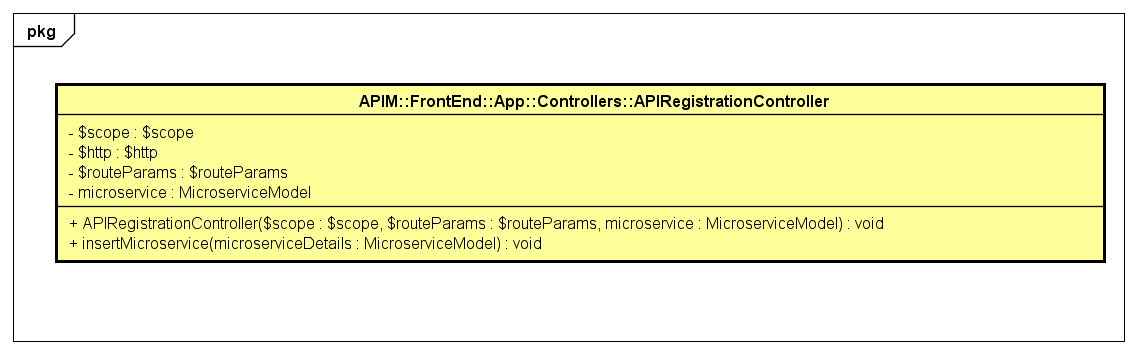
\includegraphics
	[width=0.7\linewidth]
	{images/APIM/FrontEnd/Controllers/APIRegistrationController.png}
	\caption{APIM::FrontEnd::App::Controllers::APIRegistrationController}
\end{figure}

\begin{itemize}
	\item \textbf{Descrizione:} APIRegistrationController permette di gestire l'inserimento di una API, fornendo tutte le funzionalità atte alla corretta esposizione di un microservizio di uno sviluppatore, utente della piattaforma API Market.
	\item \textbf{Attributi:}
		\begin{itemize}
		
			\item \textbf{\$scope : \$scope}\\
			Campo dati contenente un riferimento all'oggetto \$scope creato da AngularJS, viene utilizzato come mezzo di comunicazione tra il controller e la view. Contiene gli oggetti che definiscono il model dell'applicazione;
			
			\item \textbf{\$routeParams : \$routeParams}\\
			Parametro contenente il riferimento all'oggetto globale \$routeParams creato da AngularJS. Tale servizio permette di recuperare il set di variabili presenti nell'URL;

			\item \textbf{\$http : \$http }\\
			Campo dati che contiene un riferimento al servizio \$http che permette la comunicazione con il protocollo HTTP;
				
			\item \textbf{microservice : MicroserviceModel }\\
			Campo dati che si riferisce alla classe che rappresenta il modello di un microservizio.
				
		\end{itemize}
	\item \textbf{Metodi:}
		\begin{itemize}
		
			\item \textbf{APIRegistrationController(\$scope : \$scope, \$routeParams : \$routeParams, microservice : MicroserviceModel) : void}\\
			Metodo costruttore della classe.
			\begin{description}
    			\item[\textbf{Parametri:}]
			\end{description}
			\begin{itemize}
				\item \textbf{\$scope}\\
				Parametro che contiene un riferimento all'oggetto \$scope di AngularJS, impiegato nella comunicazione tra i rispettivi view e controller. Contiene gli oggetti che definiscono i model dell'applicazione;
				
				\item \textbf{\$routeParams}\\
				Parametro che contiene il riferimento all'oggetto globale \$routeParams di AngularJS. Permette di recuperare il set di variabili presenti nell'url;
				
				\item \textbf{microservice}\\
				Parametro che rappresenta un microservizio.
			\end{itemize}
			
			\item \textbf{insertMicroservice(microserviceDetails : MicroserviceModel) : void}\\
			Metodo per registrare un nuovo microservizio in API Market. Si serve di un'operazione di un servizio esposto dal package \textbf{Services}.
			\begin{description}
    			\item[\textbf{Parametri:}]
			\end{description}
			\begin{itemize}
				\item \textbf{microserviceDetails}\\
				Parametro che rappresenta un microservizio.
			\end{itemize}
			
		\end{itemize}
	\item \textbf{Relazioni con altre classi:}
		\begin{itemize}
			\item Ricava i dati necessari dal package \textbf{Services};
			\item Gestisce il funzionamento della view \textbf{RegisterAPI};
			\item Il model \textbf{MicroserviceModel} che contiene le informazioni per rappresentare un microservizio.
		\end{itemize}
\end{itemize}

\paragraph{APIM::FrontEnd::App::Controllers::SellingPolicyController}

\begin{figure}[H]
	\centering
	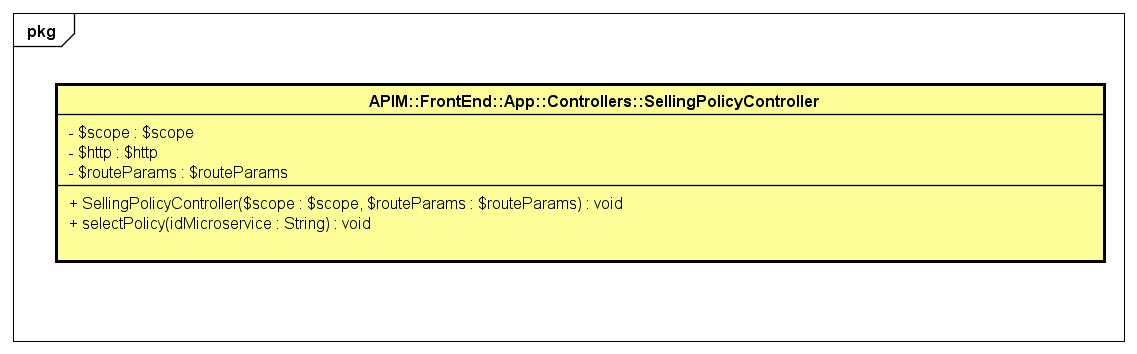
\includegraphics
	[width=0.7\linewidth]
	{images/APIM/FrontEnd/Controllers/SellingPolicyController.png}
	\caption{APIM::FrontEnd::App::Controllers::SellingPolicyController}
\end{figure}

\begin{itemize}
	\item \textbf{Descrizione:} SellingPolicyController permette di gestire le policy di vendita dei
microservizi.
	\item \textbf{Attributi:}
		\begin{itemize}
		
			\item \textbf{\$scope : \$scope}\\
			Campo dati contenente un riferimento all'oggetto \$scope creato da AngularJS, viene utilizzato come mezzo di comunicazione tra il controller e la view. Contiene gli oggetti che definiscono il model dell'applicazione;
			
			\item \textbf{\$routeParams : \$routeParams}\\
			Parametro contenente il riferimento all'oggetto globale \$routeParams creato da AngularJS. Tale servizio permette di recuperare il set di variabili presenti nell'URL;

			\item \textbf{\$http : \$http }\\
			Campo dati che contiene un riferimento al servizio \$http che permette la comunicazione con il protocollo HTTP.
				
		\end{itemize}
	\item \textbf{Metodi:}
		\begin{itemize}
		
			\item \textbf{SellingPolicyController(\$scope : \$scope, \$routeParams : \$routeParams) : void}\\
			Metodo costruttore della classe.
			\begin{description}
    			\item[\textbf{Parametri:}]
			\end{description}
			\begin{itemize}
				\item \textbf{\$scope}\\
				Parametro che contiene un riferimento all'oggetto \$scope di AngularJS, impiegato nella comunicazione tra i rispettivi view e controller. Contiene gli oggetti che definiscono i model dell'applicazione;
				
				\item \textbf{\$routeParams}\\
				Parametro che contiene il riferimento all'oggetto globale \$routeParams di AngularJS. Permette di recuperare il set di variabili presenti nell'url.
			\end{itemize}
			
			\item \textbf{selectPolicy(idMicroservice : string) : void}\\
			Metodo per selezionare una policy di vendita.
			\begin{description}
    			\item[\textbf{Parametri:}]
			\end{description}
			\begin{itemize}
				\item \textbf{idMicroservice}\\
				Parametro che contiene l'id di un microservizio.
			\end{itemize}
			
		\end{itemize}
	\item \textbf{Relazioni con altre classi:}
		\begin{itemize}
			\item Gestisce il funzionamento della view \textbf{SellingPolicy}.
		\end{itemize}
\end{itemize}

\paragraph{APIM::FrontEnd::App::Controllers::UserRegistrationController}

\begin{figure}[H]
	\centering
	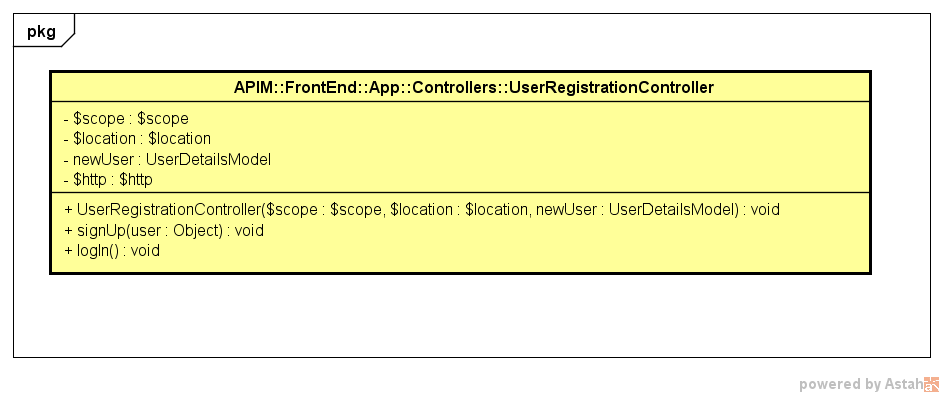
\includegraphics
	[width=0.7\linewidth]
	{images/APIM/FrontEnd/Controllers/UserRegistrationController.png}
	\caption{APIM::FrontEnd::App::Controllers::SignUpController}
\end{figure}

\begin{itemize}
	\item \textbf{Descrizione:} UserRegistrationController permette di gestire la registrazione di un
utente al sistema, fornendone le funzionalità preposte.
	\item \textbf{Attributi:}
		\begin{itemize}
		
			\item \textbf{\$scope : \$scope}\\
			Campo dati contenente un riferimento all'oggetto \$scope creato da AngularJS, viene utilizzato come mezzo di comunicazione tra il controller e la view. Contiene gli oggetti che definiscono il model dell'applicazione;
			
			\item \textbf{\$location : \$location}\\
			Campo dati contenente un riferimento al servizio creato da AngularJS che permette di accedere alla barra degli indirizzi del browser, i cambiamenti all'URL nella barra degli indirizzi si riflettono in questo oggetto e viceversa;

			\item \textbf{\$http : \$http }\\
			Campo dati che contiene un riferimento al servizio \$http che permette la comunicazione con il protocollo HTTP;
				
			\item \textbf{user : UserDetailsModel }\\
			Campo dati che si riferisce alla classe che rappresenta il modello di un utente.
				
		\end{itemize}
	\item \textbf{Metodi:}
		\begin{itemize}
		
			\item \textbf{UserRegistrationController(\$scope : \$scope, \$location : \$location, newUser : UserDetailsModel) : void}\\
			Metodo costruttore della classe;
			\begin{description}
    			\item[\textbf{Parametri:}]
			\end{description}
			\begin{itemize}
				\item \textbf{\$scope}\\
				Parametro che contiene un riferimento all'oggetto \$scope di AngularJS, impiegato nella comunicazione tra i rispettivi view e controller. Contiene gli oggetti che definiscono i model dell'applicazione;
				
				\item \textbf{\$location}\\
				Parametro che contiene un riferimento al servizio di AngularJS che permette di accedere alla barra degli indirizzi del browser, così da controllarne i cambiamenti;
				
				\item \textbf{newUser}\\
				Parametro che rappresenta un nuovo utente.
			\end{itemize}
			
			\item \textbf{signUp(user : Object) : void}\\
			Metodo per registrare un nuovo cliente in API Market. Si serve di un'operazione di un servizio esposto dal package \textbf{Services}.
			\begin{description}
    			\item[\textbf{Parametri:}]
			\end{description}
			\begin{itemize}
				\item \textbf{user}\\
				Parametro che rappresenta un utente.
			\end{itemize}
			
			\item \textbf{login() : void}\\
			Metodo per effettuare il login. Per controllare la validità dei dati immessi, si serve di un'operazione di un servizio esposto dal package \textbf{Services}.
			
		\end{itemize}
	\item \textbf{Relazioni con altre classi:}
		\begin{itemize}
			\item Ricava i dati necessari dal package \textbf{Services};
			\item Gestisce il funzionamento della view \textbf{RegisterUser};
			\item Il model \textbf{UsersDetailModel} che contiene le informazioni per rappresentare un utente.
		\end{itemize}
\end{itemize}

\paragraph{APIM::FrontEnd::App::Controllers::APIRegisteredController}

\begin{figure}[H]
	\centering
	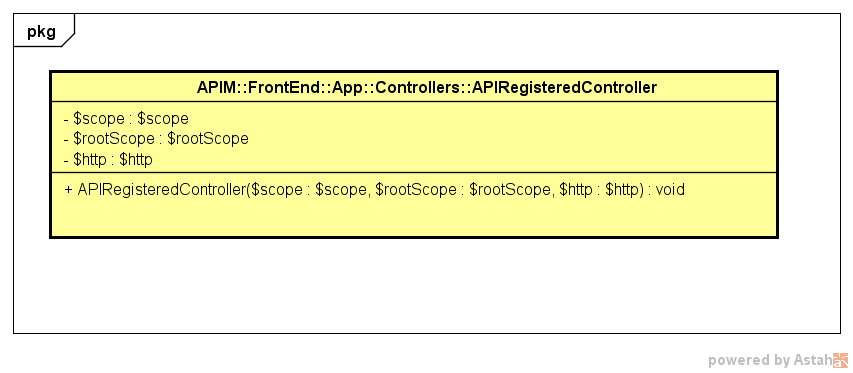
\includegraphics
	[width=0.7\linewidth]
	{images/APIM/FrontEnd/Controllers/APIRegisteredController.png}
	\caption{APIM::FrontEnd::App::Controllers::APIRegisteredController}
\end{figure}

\begin{itemize}
	\item \textbf{Descrizione:} APIRegisteredController permette di gestire le informazioni di una
API precedentemente inserita.
	\item \textbf{Attributi:}
		\begin{itemize}
		
			\item \textbf{\$scope : \$scope}\\
			Campo dati contenente un riferimento all'oggetto \$scope creato da AngularJS, viene utilizzato come mezzo di comunicazione tra il controller e la view. Contiene gli oggetti che definiscono il model dell'applicazione;
			
			\item \textbf{\$rootScope : \$rootScope}\\
			Campo dati contenente il riferimento all'oggetto globale \$rootScope creato da AngularJS. Viene utilizzato per rendere accessibile a tutti i controllers e a tutte le views l'oggetto MicroserviceModel;

			\item \textbf{\$http : \$http }\\
			Campo dati che contiene un riferimento al servizio \$http che permette la comunicazione con il protocollo HTTP;
				
			\item \textbf{microservice : MicroserviceModel }\\
			Campo dati che si riferisce alla classe che rappresenta il modello di un microservizio.
				
		\end{itemize}
	\item \textbf{Metodi:}
		\begin{itemize}
		
			\item \textbf{APIRegisteredController(\$scope : \$scope, \$rootScope : \$rootScope, microservice : MicroserviceModel) : void}\\
			Metodo costruttore della classe;
			\begin{description}
    			\item[\textbf{Parametri:}]
			\end{description}
			\begin{itemize}
				\item \textbf{\$scope}\\
				Parametro che contiene un riferimento all'oggetto \$scope di AngularJS, impiegato nella comunicazione tra i rispettivi view e controller. Contiene gli oggetti che definiscono i model dell'applicazione;
				
				\item \textbf{\$rootScope}\\
				Parametro che contiene il riferimento all'oggetto globale \$rootScope di AngularJS. Viene utilizzato per rendere accessibile a view e controller l'oggetto MicroserviceModel;
				
				\item \textbf{microservice}\\
				Parametro che rappresenta un microservizio.
			\end{itemize}
			
			\item \textbf{getMicroservicesDetails(email : string) : Array<MicroserviceModel>}\\
			Metodo per visualizzare le informazioni di un proprio microservizio registrato. Si serve di un'operazione di un servizio esposto dal package \textbf{Services};
			\begin{description}
    			\item[\textbf{Parametri:}]
			\end{description}
			\begin{itemize}
				\item \textbf{email}\\
				Parametro che rappresenta un indirizzo email.
			\end{itemize}
			
			\item \textbf{setMicroservice(newInfo : MicroserviceModel) : void}\\
			Metodo per modificare le informazioni di un proprio microservizio registrato. Si serve di un'operazione di un servizio esposto dal package \textbf{Services}.
			\begin{description}
    			\item[\textbf{Parametri:}]
			\end{description}
			\begin{itemize}
				\item \textbf{newInfo}\\
				Parametro che rappresenta un microservizio aggiornato.
			\end{itemize}

		\end{itemize}
	\item \textbf{Relazioni con altre classi:}
		\begin{itemize}
			\item Ricava i dati necessari dal package \textbf{Services};
			\item Gestisce il funzionamento della view \textbf{APIRegistered};
			\item Il model \textbf{MicroserviceModel} che contiene le informazioni per rappresentare un microservizio.
		\end{itemize}
\end{itemize}

\paragraph{APIM::FrontEnd::App::Controllers::SearchController}

\begin{figure}[H]
	\centering
	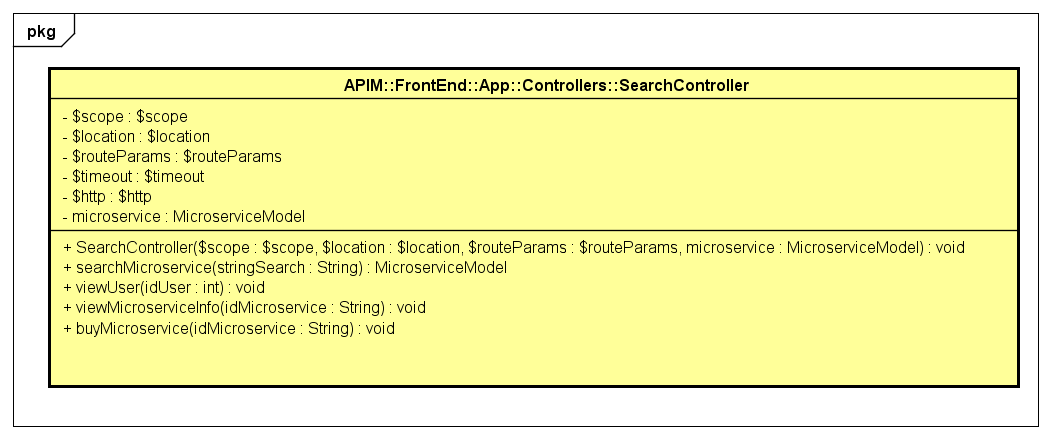
\includegraphics
	[width=0.7\linewidth]
	{images/APIM/FrontEnd/Controllers/SearchController.png}
	\caption{APIM::FrontEnd::App::Controllers::SearchController}
\end{figure}

\begin{itemize}
	\item \textbf{Descrizione:} SearchController permette di gestire la ricerca di microservizi all'interno
di API Market, fornendo all'utente le funzionalità di ricerca tramite
categorie e keywords per sviluppatori e microservizi.
	\item \textbf{Attributi:}
		\begin{itemize}
		
			\item \textbf{\$scope : \$scope}\\
			Campo dati contenente un riferimento all'oggetto \$scope creato da AngularJS, viene utilizzato come mezzo di comunicazione tra il controller e la view. Contiene gli oggetti che definiscono il model dell'applicazione;

			\item \textbf{\$routeParams : \$routeParams}\\
			Parametro contenente il riferimento all'oggetto globale \$routeParams creato da AngularJS. Tale servizio permette di recuperare il set di variabili presenti nell'URL.			
			
			\item \textbf{\$location : \$location}\\
			Campo dati contenente un riferimento al servizio creato da AngularJS che permette di accedere alla barra degli indirizzi del browser, i cambiamenti all'URL nella barra degli indirizzi si riflettono in questo oggetto e viceversa;
			
			\item \textbf{\$rootScope : \$rootScope}\\
			Campo dati contenente il riferimento all'oggetto globale \$rootScope creato da AngularJS. Viene utilizzato per rendere accessibile a tutti i controllers e a tutte le views l'oggetto MicroserviceModel;
			
			\item \textbf{\$timeout : \$timeout }\\
			Campo dati contenente il riferimento all'oggetto globale \$timeout creato da AngularJS. Il valore di ritorno di una chiamata alla funzione di \$timeout è una promise, la quale sarà risolta quando avverrà il ritardo e la funzione di timeout eseguita;

			\item \textbf{\$http : \$http }\\
			Campo dati che contiene un riferimento al servizio \$http che permette la comunicazione con il protocollo HTTP;
				
			\item \textbf{microservice : MicroserviceModel }\\
			Campo dati che si riferisce alla classe che rappresenta il modello di un microservizio.
				
		\end{itemize}
	\item \textbf{Metodi:}
		\begin{itemize}
		
			\item \textbf{SearchController(\$scope : \$scope, \$location : \$location, \$routeParams : \$routeParams, microservice : MicroserviceModel) : void}\\
			Metodo costruttore della classe;
			\begin{description}
    			\item[\textbf{Parametri:}]
			\end{description}
			\begin{itemize}
				\item \textbf{\$scope}\\
				Parametro che contiene un riferimento all'oggetto \$scope di AngularJS, impiegato nella comunicazione tra i rispettivi view e controller. Contiene gli oggetti che definiscono i model dell'applicazione;
				
				\item \textbf{\$location}\\
				Parametro che contiene un riferimento al servizio di AngularJS che permette di accedere alla barra degli indirizzi del browser, così da controllarne i cambiamenti;
				
				\item \textbf{\$routeParams}\\
				Parametro che contiene il riferimento all'oggetto globale \$routeParams di AngularJS. Permette di recuperare il set di variabili presenti nell'url;
				
				\item \textbf{microservice}\\
				Parametro che rappresenta un microservizio.
			\end{itemize}
			
			\item \textbf{searchMicroservice(stringSearch : string) : MicroserviceModel}\\
			Metodo per la ricerca della lista di API che corrispondono alle keywords immesse. Si serve di un'operazione di un servizio esposto dal package \textbf{Services}.
			\begin{description}
    			\item[\textbf{Parametri:}]
			\end{description}
			\begin{itemize}
				\item \textbf{stringSearch}\\
				Parametro che rappresenta una stringa di keywords di ricerca.
			\end{itemize}
			
			\item \textbf{viewUser(idUser : int) : void}\\
			Metodo per visualizzare la pagina dell'utente di una specifica API. Si serve di un'operazione di un servizio esposto dal package \textbf{Services}.
			\begin{description}
    			\item[\textbf{Parametri:}]
			\end{description}
			\begin{itemize}
				\item \textbf{idUser}\\
				Parametro che rappresenta l'id di un utente da visualizzare.
			\end{itemize}
			
			\item \textbf{viewMicroserviceInfo(idMicroservice : string) : void}\\
			Metodo per visualizzare la pagina dell'API di una specifica API della lista dei risultati della ricerca. Si serve di un'operazione di un servizio esposto dal package \textbf{Services}.
			\begin{description}
    			\item[\textbf{Parametri:}]
			\end{description}
			\begin{itemize}
				\item \textbf{idMicroservice}\\
				Parametro che rappresenta l'id di un microservizio da visualizzare.
			\end{itemize}
			
			\item \textbf{buyMicroservice(idMicroservice : string) : void}\\
			Metodo per iniziare l'acquisto di una specifica API. Si serve della procedura di acquisto di PayPal.
			\begin{description}
    			\item[\textbf{Parametri:}]
			\end{description}
			\begin{itemize}
				\item \textbf{idMicroservice}\\
				Parametro che rappresenta l'id di un microservizio da acquistare.
			\end{itemize}
			
		\end{itemize}
	\item \textbf{Relazioni con altre classi:}
		\begin{itemize}
			\item Ricava i dati necessari dal package \textbf{Services};
			\item Gestisce il funzionamento della view \textbf{API};
			\item Il model \textbf{MicroserviceModel} che contiene le informazioni per rappresentare un microservizio.
		\end{itemize}
\end{itemize}

\paragraph{APIM::FrontEnd::App::Controllers::TransactionsListController}

\begin{figure}[H]
	\centering
	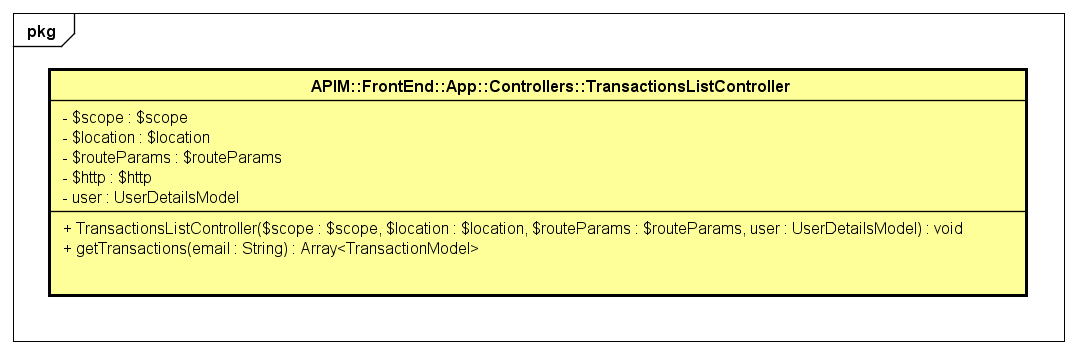
\includegraphics
	[width=0.7\linewidth]
	{images/APIM/FrontEnd/Controllers/TransactionsListController.png}
	\caption{APIM::FrontEnd::App::Controllers::TransactionsListController}
\end{figure}

\begin{itemize}
	\item \textbf{Descrizione:} TransactionsListController permette di gestire lo storico delle transazioni
di un utente di API Market.
	\item \textbf{Attributi:}
		\begin{itemize}
		
			\item \textbf{\$scope : \$scope}\\
			Campo dati contenente un riferimento all'oggetto \$scope creato da AngularJS, viene utilizzato come mezzo di comunicazione tra il controller e la view. Contiene gli oggetti che definiscono il model dell'applicazione;

			\item \textbf{\$routeParams : \$routeParams}\\
			Parametro contenente il riferimento all'oggetto globale \$routeParams creato da AngularJS. Tale servizio permette di recuperare il set di variabili presenti nell'URL.			
			
			\item \textbf{\$location : \$location}\\
			Campo dati contenente un riferimento al servizio creato da AngularJS che permette di accedere alla barra degli indirizzi del browser, i cambiamenti all'URL nella barra degli indirizzi si riflettono in questo oggetto e viceversa;
			
			\item \textbf{\$rootScope : \$rootScope}\\
			Campo dati contenente il riferimento all'oggetto globale \$rootScope creato da AngularJS. Viene utilizzato per rendere accessibile a tutti i controllers e a tutte le views l'oggetto TransactionModel;

			\item \textbf{\$http : \$http }\\
			Campo dati che contiene un riferimento al servizio \$http che permette la comunicazione con il protocollo HTTP;
				
			\item \textbf{transaction : TransactionModel }\\
			Campo dati che si riferisce alla classe che rappresenta il modello di una transazione.
				
		\end{itemize}
	\item \textbf{Metodi:}
		\begin{itemize}
		
			\item \textbf{TransactionsListController(\$scope : \$scope, \$location : \$location, \$routeParams : \$routeParams, user : UserDetailsModel) : void}\\
			Metodo costruttore della classe;
			\begin{description}
    			\item[\textbf{Parametri:}]
			\end{description}
			\begin{itemize}
				\item \textbf{\$scope}\\
				Parametro che contiene un riferimento all'oggetto \$scope di AngularJS, impiegato nella comunicazione tra i rispettivi view e controller. Contiene gli oggetti che definiscono i model dell'applicazione;
				\item \textbf{\$location}\\
				Parametro che contiene un riferimento al servizio di AngularJS che permette di accedere alla barra degli indirizzi del browser, così da controllarne i cambiamenti;
			
				\item \textbf{\$routeParams}\\
				Parametro che contiene il riferimento all'oggetto globale \$routeParams di AngularJS. Permette di recuperare il set di variabili presenti nell'url;
				
				\item \textbf{user}\\
				Parametro che rappresenta un utente.
			\end{itemize}
			
			\item \textbf{getTransactions(email : string) : Array<TransactionModel>}\\
			Metodo per visualizzare la lista delle transazioni di un utente. Si serve di un'operazione di un servizio esposto dal package \textbf{Services}.
			\begin{description}
    			\item[\textbf{Parametri:}]
			\end{description}
			\begin{itemize}
				\item \textbf{email}\\
				Parametro che contiene un indirizzo email.
			\end{itemize}
			
		\end{itemize}
	\item \textbf{Relazioni con altre classi:}
		\begin{itemize}
			\item Ricava i dati necessari dal package \textbf{Services};
			\item Gestisce il funzionamento della view \textbf{TransactionsList};
			\item Il model \textbf{UserDetailsModel} che contiene le informazioni per rappresentare un utente.
			\item Il model \textbf{TransactionModel} che contiene le informazioni per rappresentare una transazione.
		\end{itemize}
\end{itemize}

\paragraph{APIM::FrontEnd::App::Controllers::AdminManagerController}

\begin{figure}[H]
	\centering
	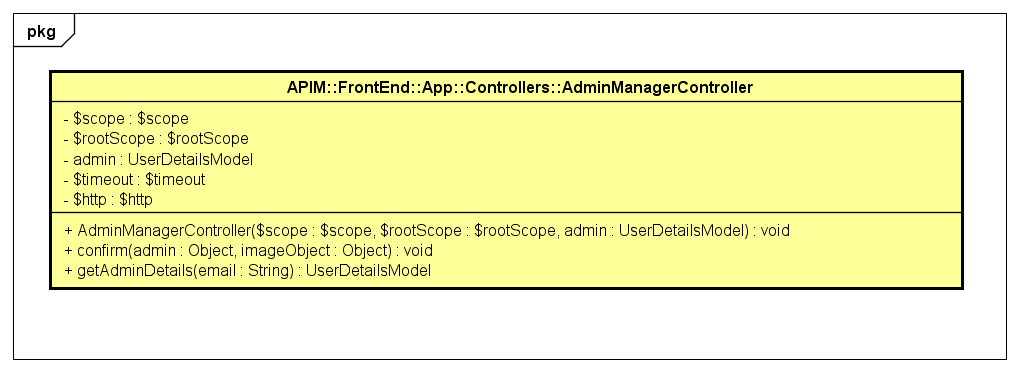
\includegraphics
	[width=0.7\linewidth]
	{images/APIM/FrontEnd/Controllers/AdminManagerController.png}
	\caption{APIM::FrontEnd::App::Controllers::AdminManagerController}
\end{figure}

\begin{itemize}
	\item \textbf{Descrizione:} AdminManagerController permette di gestire il profilo di un amministratore della piattaforma API Market, fornendo le funzionalità per poter modificare i propri dati e moderare utenti ed API.
	\item \textbf{Attributi:}
		\begin{itemize}
		
			\item \textbf{\$scope : \$scope}\\
			Campo dati contenente un riferimento all'oggetto \$scope creato da AngularJS, viene utilizzato come mezzo di comunicazione tra il controller e la view. Contiene gli oggetti che definiscono il model dell'applicazione;
			
			\item \textbf{\$rootScope : \$rootScope}\\
			Campo dati contenente il riferimento all'oggetto globale \$rootScope creato da AngularJS. Viene utilizzato per rendere accessibile a tutti i controllers e a tutte le views l'oggetto UserDetailsModel;
			
			\item \textbf{\$timeout : \$timeout }\\
			Campo dati contenente il riferimento all'oggetto globale \$timeout creato da AngularJS. Il valore di ritorno di una chiamata alla funzione di \$timeout è una promise, la quale sarà risolta quando avverrà il ritardo e la funzione di timeout eseguita;

			\item \textbf{\$http : \$http }\\
			Campo dati che contiene un riferimento al servizio \$http che permette la comunicazione con il protocollo HTTP;
				
			\item \textbf{admin : UserDetailsModel }\\
			Campo dati che si riferisce alla classe che rappresenta il modello di un utente.
				
		\end{itemize}
	\item \textbf{Metodi:}
		\begin{itemize}
		
			\item \textbf{AdminManagerController(\$scope : \$scope, \$rootScope : \$rootScope, admin : UserDetailsModel) : void}\\
			Metodo costruttore della classe.
			\begin{description}
    			\item[\textbf{Parametri:}]
			\end{description}
			\begin{itemize}
				\item \textbf{\$scope}\\
				Parametro che contiene un riferimento all'oggetto \$scope di AngularJS, impiegato nella comunicazione tra i rispettivi view e controller. Contiene gli oggetti che definiscono i model dell'applicazione;
				
				\item \textbf{\$rootScope}\\
				Parametro che contiene il riferimento all'oggetto globale \$rootScope di AngularJS. Viene utilizzato per rendere accessibile a view e controller l'oggetto UserDetailsModel;
				
				\item \textbf{admin}\\
				Parametro che rappresenta un admin.
			\end{itemize}
			
			\item \textbf{confirm(admin : Object, imageObject : Object) : void}\\
			Metodo per confermare le modifiche desiderate al profilo admin. Si serve di un'operazione di un servizio esposto dal package \textbf{Services};
			\begin{description}
    			\item[\textbf{Parametri:}]
			\end{description}
			\begin{itemize}
				\item \textbf{admin}\\
				Parametro che rappresenta un admin;
				
				\item \textbf{imageObject}\\
				Parametro che rappresenta un file immagine.
			\end{itemize}
			
			\item \textbf{getAdminDetails(email : string) : UserDetailsModel}\\
			Metodo per visualizzare le informazioni personali del profilo admin. Si serve di un'operazione di un servizio esposto dal package \textbf{Services}.
			\begin{description}
    			\item[\textbf{Parametri:}]
			\end{description}
			\begin{itemize}
				\item \textbf{email}\\
				Parametro che rappresenta un indirizzo email;
			\end{itemize}
			
		\end{itemize}
	\item \textbf{Relazioni con altre classi:}
		\begin{itemize}
			\item Ricava i dati necessari dal package \textbf{Services};
			\item Gestisce il funzionamento della view \textbf{AdminManager};
			\item Il model \textbf{UsersDetailModel} che contiene le informazioni per rappresentare un utente.
		\end{itemize}
\end{itemize}

\paragraph{APIM::FrontEnd::App::Controllers::AdminModerationController}

\begin{figure}[H]
	\centering
	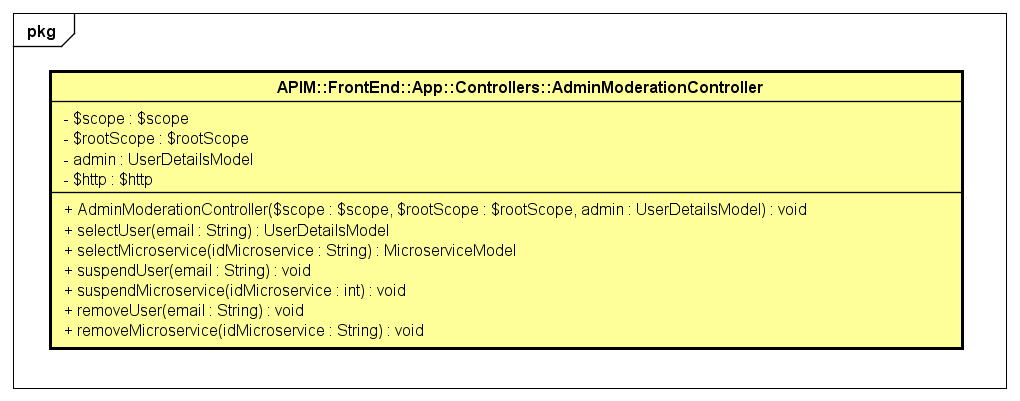
\includegraphics
	[width=0.7\linewidth]
	{images/APIM/FrontEnd/Controllers/AdminModerationController.png}
	\caption{APIM::FrontEnd::App::Controllers::AdminModerationController}
\end{figure}

\begin{itemize}
	\item \textbf{Descrizione:} AdminModerationController permette di gestire la moderazione di
un utente (cliente o sviluppatore che sia) e di API, fornendo le funzionalità per la
sospensione e rimozione.
	\item \textbf{Attributi:}
		\begin{itemize}
		
			\item \textbf{\$scope : \$scope}\\
			Campo dati contenente un riferimento all'oggetto \$scope creato da AngularJS, viene utilizzato come mezzo di comunicazione tra il controller e la view. Contiene gli oggetti che definiscono il model dell'applicazione;
			
			\item \textbf{\$rootScope : \$rootScope}\\
			Campo dati contenente il riferimento all'oggetto globale \$rootScope creato da AngularJS. Viene utilizzato per rendere accessibile a tutti i controllers e a tutte le views gli oggetti UserDetailsModel e MicroserviceModel;

			\item \textbf{\$http : \$http }\\
			Campo dati che contiene un riferimento al servizio \$http che permette la comunicazione con il protocollo HTTP;
				
			\item \textbf{admin : UserDetailsModel }\\
			Campo dati che si riferisce alla classe che rappresenta il modello di un utente.
			
			\item \textbf{microservice : MicroserviceModel }\\
			Campo dati che si riferisce alla classe che rappresenta il modello di un microservizio.
				
		\end{itemize}
	\item \textbf{Metodi:}
		\begin{itemize}
		
			\item \textbf{AdminManagerController(\$scope : \$scope, \$rootScope : \$rootScope, admin : UserDetailsModel) : void}\\
			Metodo costruttore della classe.
			\begin{description}
    			\item[\textbf{Parametri:}]
			\end{description}
			\begin{itemize}
				\item \textbf{\$scope}\\
				Parametro che contiene un riferimento all'oggetto \$scope di AngularJS, impiegato nella comunicazione tra i rispettivi view e controller. Contiene gli oggetti che definiscono i model dell'applicazione;
				
				\item \textbf{\$rootScope}\\
				Parametro che contiene il riferimento all'oggetto globale \$rootScope di AngularJS. Viene utilizzato per rendere accessibile a view e controller l'oggetto UserDetailsModel;
				
				\item \textbf{admin}\\
				Parametro che rappresenta un admin.
			\end{itemize}
			
			\item \textbf{selectUser(email : string) : UserDetailsModel}\\
			Metodo per selezionare un utente da moderare.
			\begin{description}
    			\item[\textbf{Parametri:}]
			\end{description}
			\begin{itemize}
				\item \textbf{email}\\
				Parametro che rappresenta un indirizzo email.
			\end{itemize}
			
			\item \textbf{selectMicroservice(idMicroservice : string) : MicroserviceModel}\\
			Metodo per selezionare una API da moderare.
			\begin{description}
    			\item[\textbf{Parametri:}]
			\end{description}
			\begin{itemize}
				\item \textbf{idMicroservice}\\
				Parametro che rappresenta l'id di un microservizio.
			\end{itemize}
			
			\item \textbf{suspendUser(email : string) : void}\\
			Metodo per sospendere l'utente selezionato. Si serve di un'operazione di un servizio esposto dal package \textbf{Services}.
			\begin{description}
    			\item[\textbf{Parametri:}]
			\end{description}
			\begin{itemize}
				\item \textbf{email}\\
				Parametro che rappresenta un indirizzo email.
			\end{itemize}
			
			\item \textbf{suspendMicroservice(idMicroservice : int) : void}\\
			Metodo per sospendere l'API selezionata. Si serve di un'operazione di un servizio esposto dal package \textbf{Services}.
			\begin{description}
    			\item[\textbf{Parametri:}]
			\end{description}
			\begin{itemize}
				\item \textbf{idMicroservice}\\
				Parametro che rappresenta l'id di un microservizio.
			\end{itemize}
			
			\item \textbf{removeUser(email : string) : void}\\
			Metodo per cancellare l'utente selezionato. Si serve di un'operazione di un servizio esposto dal package \textbf{Services}.
			\begin{description}
    			\item[\textbf{Parametri:}]
			\end{description}
			\begin{itemize}
				\item \textbf{email}\\
				Parametro che rappresenta un indirizzo email.
			\end{itemize}
			
			\item \textbf{removeMicroservice(idMicroservice : string) : void}\\
			Metodo per disabilitare il microservizio selezionato. Si serve di un'operazione di un servizio esposto dal package \textbf{Services}.
			\begin{description}
    			\item[\textbf{Parametri:}]
			\end{description}
			\begin{itemize}
				\item \textbf{idMicroservice}\\
				Parametro che rappresenta l'id di un microservizio.
			\end{itemize}
			
		\end{itemize}
	\item \textbf{Relazioni con altre classi:}
		\begin{itemize}
			\item Ricava i dati necessari dal package \textbf{Services};
			\item Gestisce il funzionamento della view \textbf{AdminModeration};
			\item Il model \textbf{UsersDetailModel} che contiene le informazioni per rappresentare un utente;
			\item Il model \textbf{MicroserviceModel} che contiene le informazioni per rappresentare un microservizio.
	\end{itemize}
\end{itemize}

\paragraph{APIM::FrontEnd::App::Controllers::LoginController}

\begin{figure}[H]
	\centering
	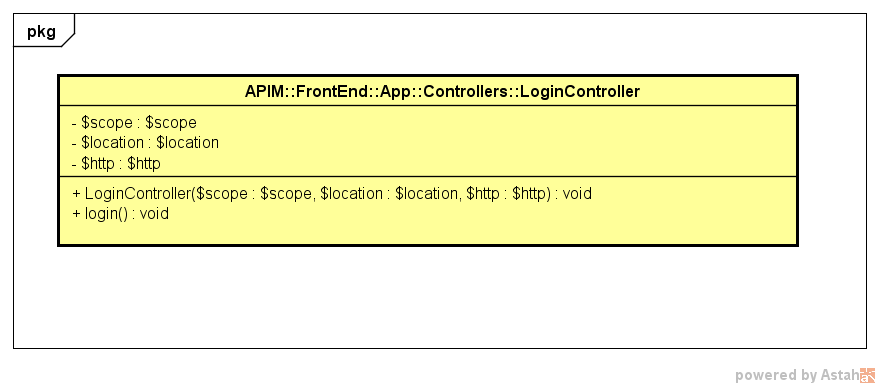
\includegraphics
	[width=0.7\linewidth]
	{images/APIM/FrontEnd/Controllers/LoginController.png}
	\caption{APIM::FrontEnd::App::Controllers::LoginController}
\end{figure}

\begin{itemize}
	\item \textbf{Descrizione:} LoginController permette di gestire il login di un utente alla piattaforma
API Market, fornendo le funzionalità di autenticazione al sistema, compresa la gestione di situazioni di errore di autenticazione.
	\item \textbf{Attributi:}
		\begin{itemize}
		
			\item \textbf{\$scope : \$scope}\\
			Campo dati contenente un riferimento all'oggetto \$scope creato da AngularJS, viene utilizzato come mezzo di comunicazione tra il controller e la view. Contiene gli oggetti che definiscono il model dell'applicazione;
			
			\item \textbf{\$rootScope : \$rootScope}\\
			Campo dati contenente il riferimento all'oggetto globale \$rootScope creato da AngularJS. Viene utilizzato per rendere accessibile a tutti i controllers e a tutte le views l'oggetto UserDetailsModel;
			
			\item \textbf{\$location : \$location}\\
			Campo dati contenente un riferimento al servizio creato da AngularJS che permette di accedere alla barra degli indirizzi del browser, i cambiamenti all'URL nella barra degli indirizzi si riflettono in questo oggetto e viceversa;

			\item \textbf{\$http : \$http }\\
			Campo dati che contiene un riferimento al servizio \$http che permette la comunicazione con il protocollo HTTP;
				
			\item \textbf{newUser : UserDetailsModel }\\
			Campo dati che si riferisce alla classe che rappresenta il modello di un utente.
				
		\end{itemize}
	\item \textbf{Metodi:}
		\begin{itemize}
		
			\item \textbf{LoginController(\$scope : \$scope, \$rootScope : \$rootScope, \$location : \$location, user : UserDetailsModel) : void}\\
			Metodo costruttore della classe.
			\begin{description}
    			\item[\textbf{Parametri:}]
			\end{description}
			\begin{itemize}
				\item \textbf{\$scope}\\
				Parametro che contiene un riferimento all'oggetto \$scope di AngularJS, impiegato nella comunicazione tra i rispettivi view e controller. Contiene gli oggetti che definiscono i model dell'applicazione;
				
				\item \textbf{\$rootScope}\\
				Parametro che contiene il riferimento all'oggetto globale \$rootScope di AngularJS. Viene utilizzato per rendere accessibile a view e controller l'oggetto UserDetailsModel;
				
				\item \textbf{\$location}\\
				Parametro che contiene un riferimento al servizio di AngularJS che permette di accedere alla barra degli indirizzi del browser, così da controllarne i cambiamenti;
				
				\item \textbf{user}\\
				Parametro che rappresenta un utente.
			\end{itemize}
			
			\item \textbf{logIn(email : string, password : string) : void}\\
			Metodo per effettuare il login. Per verificare la validità dei dati immessi, si serve di un'operazione di un servizio esposto dal package \textbf{Services}.
			\begin{description}
    			\item[\textbf{Parametri:}]
			\end{description}
			\begin{itemize}
				\item \textbf{email}\\
				Parametro che rappresenta un indirizzo email;
				
				\item \textbf{password}\\
				Parametro che rappresenta una password.
			\end{itemize}
			
			\item \textbf{registration() : void}\\
			Metodo per registrare un nuovo account utente. Si serve di un'operazione di un servizio esposto dal package \textbf{Services}.
			
			\item \textbf{recoveryPassword() : void}\\
			Metodo per recuperare la password di un utente. Per verificare l'esistenza dell'utente sbadato e per aggiornarne la password, si serve delle operazioni dei servizi esposti dal package \textbf{Services}.
			
		\end{itemize}
	\item \textbf{Relazioni con altre classi:}
		\begin{itemize}
			\item Ricava i dati necessari dal package \textbf{Services};
			\item Gestisce il funzionamento della view \textbf{Login};
			\item Il model \textbf{UsersDetailModel} che contiene le informazioni per rappresentare un utente.
		\end{itemize}
\end{itemize}

\paragraph{APIM::FrontEnd::App::Controllers::VirtualAccountController}

\begin{figure}[H]
	\centering
	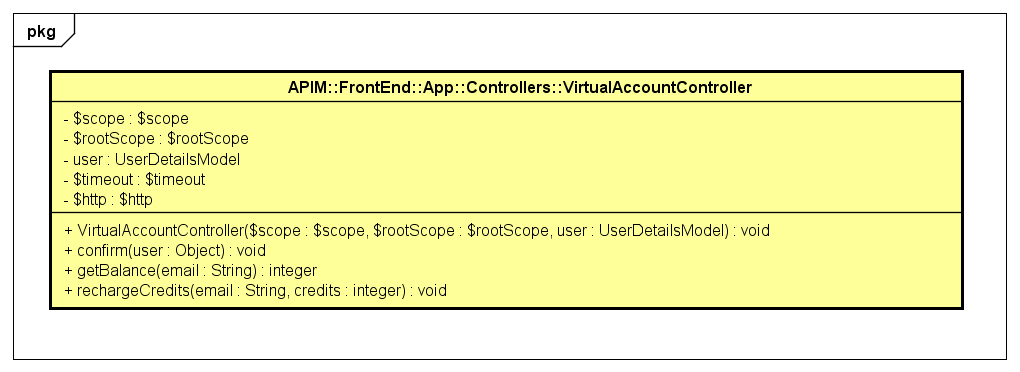
\includegraphics
	[width=0.7\linewidth]
	{images/APIM/FrontEnd/Controllers/VirtualAccountController.png}
	\caption{APIM::Front-End::App::Controllers::VirtualAccountController}
\end{figure}

\begin{itemize}
	\item \textbf{Descrizione:} VirtualAccountController permette di gestire il conto virtuale associato
al profilo di un utente, fornendo le funzionalità per la ricarica del saldo tramite PayPal.
	\item \textbf{Attributi:}
		\begin{itemize}
		
			\item \textbf{\$scope : \$scope}\\
			Campo dati contenente un riferimento all'oggetto \$scope creato da AngularJS, viene utilizzato come mezzo di comunicazione tra il controller e la view. Contiene gli oggetti che definiscono il model dell'applicazione;
			
			\item \textbf{\$rootScope : \$rootScope}\\
			Campo dati contenente il riferimento all'oggetto globale \$rootScope creato da AngularJS. Viene utilizzato per rendere accessibile a tutti i controllers e a tutte le views gli oggetti UserDetailsModel e TransactionModel;
			
			\item \textbf{\$location : \$location}\\
			Campo dati contenente un riferimento al servizio creato da AngularJS che permette di accedere alla barra degli indirizzi del browser, i cambiamenti all'URL nella barra degli indirizzi si riflettono in questo oggetto e viceversa;

			\item \textbf{\$http : \$http }\\
			Campo dati che contiene un riferimento al servizio \$http che permette la comunicazione con il protocollo HTTP;
				
			\item \textbf{user : UserDetailsModel }\\
			Campo dati che si riferisce alla classe che rappresenta il modello di un utente.
			
			\item \textbf{transaction : TransactionModel }\\
			Campo dati che si riferisce alla classe che rappresenta il modello di una transazione.
				
		\end{itemize}
	\item \textbf{Metodi:}
		\begin{itemize}
		
			\item \textbf{VirtualAccountController(\$scope : \$scope, \$rootScope : \$rootScope, user : UserDetailsModel) : void}\\
			Metodo costruttore della classe.
			\begin{description}
    			\item[\textbf{Parametri:}]
			\end{description}
			\begin{itemize}
				\item \textbf{\$scope}\\
				Parametro che contiene un riferimento all'oggetto \$scope di AngularJS, impiegato nella comunicazione tra i rispettivi view e controller. Contiene gli oggetti che definiscono i model dell'applicazione;
				
				\item \textbf{\$rootScope}\\
				Parametro che contiene il riferimento all'oggetto globale \$rootScope di AngularJS. Viene utilizzato per rendere accessibile a view e controller l'oggetto UserDetailsModel;
				
				\item \textbf{user}\\
				Parametro che rappresenta un utente.
			\end{itemize}
			
			\item \textbf{confirm(user : Object) : void}\\
			Metodo per confermare la ricarica dei crediti del conto virtuale dell'utente. Si serve di un'operazione di un servizio esposto dal package \textbf{Services}.
			\begin{description}
    			\item[\textbf{Parametri:}]
			\end{description}
			\begin{itemize}
				\item \textbf{user}\\
				Parametro che rappresenta un utente.
			\end{itemize}
			
			\item \textbf{getBalance(email : string) : int}\\
			Metodo per visualizzare il saldo attuale dei crediti dell'utente. Si serve di un'operazione di un servizio esposto dal package \textbf{Services}.
			\begin{description}
    			\item[\textbf{Parametri:}]
			\end{description}
			\begin{itemize}
				\item \textbf{email}\\
				Parametro che rappresenta un indirizzo email.
			\end{itemize}
			
			\item \textbf{rechargeCredits(email : string, credits : int) : void}\\
			Metodo per ricaricare i crediti del conto virtuale dell'utente. Si serve di un'operazione di un servizio esposto dal package \textbf{Services}.
			\begin{description}
    			\item[\textbf{Parametri:}]
			\end{description}
			\begin{itemize}
				\item \textbf{email}\\
				Parametro che rappresenta un indirizzo email;
				
				\item \textbf{credits}\\
				Parametro che rappresenta il numbero di crediti da acquistare;
			\end{itemize}
			
		\end{itemize}
	\item \textbf{Relazioni con altre classi:}
		\begin{itemize}
			\item Ricava i dati necessari dal package \textbf{Services};
			\item Gestisce il funzionamento della view \textbf{VirtualAccount};
			\item Il model \textbf{UsersDetailModel} che contiene le informazioni per rappresentare un utente.
		\end{itemize}
\end{itemize}

\paragraph{APIM::FrontEnd::App::Controllers::PasswordRecoveryController}

\begin{figure}[H]
	\centering
	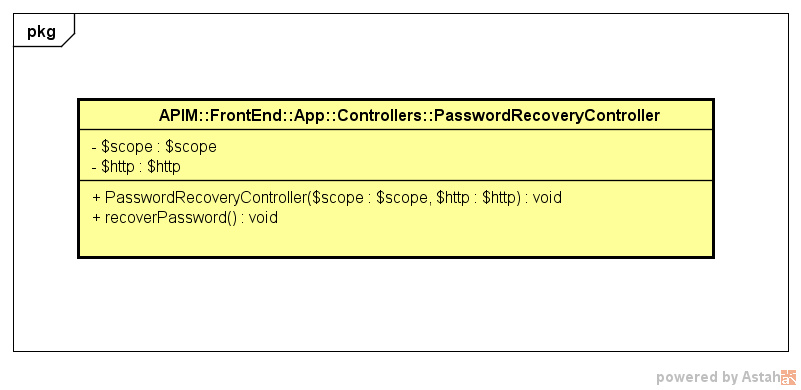
\includegraphics
	[width=0.7\linewidth]
	{images/APIM/FrontEnd/Controllers/PasswordRecoveryController.png}
	\caption{APIM::FrontEnd::App::Controllers::PasswordRecoveryController}
\end{figure}

\begin{itemize}
	\item \textbf{Descrizione:} PasswordRecoveryController permette di gestire il ripristino della password
dimenticata da un utente, fornendo tutte le funzionalità per il recupero della password dopo aver verificato l'identità dell'utente.
	\item \textbf{Attributi:}
		\begin{itemize}
		
			\item \textbf{\$scope : \$scope}\\
			Campo dati contenente un riferimento all'oggetto \$scope creato da AngularJS, viene utilizzato come mezzo di comunicazione tra il controller e la view. Contiene gli oggetti che definiscono il model dell'applicazione;
			
			\item \textbf{\$rootScope : \$rootScope}\\
			Campo dati contenente il riferimento all'oggetto globale \$rootScope creato da AngularJS. Viene utilizzato per rendere accessibile a tutti i controllers e a tutte le views l'oggetto UserDetailsModel;
			
			\item \textbf{\$location : \$location}\\
			Campo dati contenente un riferimento al servizio creato da AngularJS che permette di accedere alla barra degli indirizzi del browser, i cambiamenti all'URL nella barra degli indirizzi si riflettono in questo oggetto e viceversa;

			\item \textbf{\$http : \$http }\\
			Campo dati che contiene un riferimento al servizio \$http che permette la comunicazione con il protocollo HTTP;
				
			\item \textbf{user : UserDetailsModel }\\
			Campo dati che si riferisce alla classe che rappresenta il modello di un utente.

		\end{itemize}
	\item \textbf{Metodi:}
		\begin{itemize}
		
			\item \textbf{PasswordRecoveryController(\$scope : \$scope, \$location : \$location) : void}\\
			Metodo costruttore della classe.
			\begin{description}
    			\item[\textbf{Parametri:}]
			\end{description}
			\begin{itemize}
				\item \textbf{\$scope}\\
				Parametro che contiene un riferimento all'oggetto \$scope di AngularJS, impiegato nella comunicazione tra i rispettivi view e controller. Contiene gli oggetti che definiscono i model dell'applicazione;
				
				\item \textbf{\$location}\\
				Parametro che contiene un riferimento al servizio di AngularJS che permette di accedere alla barra degli indirizzi del browser, così da controllarne i cambiamenti.
				
			\end{itemize}
			
			\item \textbf{passwordForgot() : void}\\
			Metodo per recuperare la password dell'utente. Per aggiornare la nuova password, si serve di un'operazione di un servizio esposto dal package \textbf{Services}.
			
		\end{itemize}
	\item \textbf{Relazioni con altre classi:}
		\begin{itemize}
			\item Ricava i dati necessari dal package \textbf{Services};
			\item Gestisce il funzionamento della view \textbf{PasswordRecovery}.
		\end{itemize}
\end{itemize}

\paragraph{APIM::FrontEnd::App::Controllers::ResetPasswordController}

\begin{figure}[H]
	\centering
	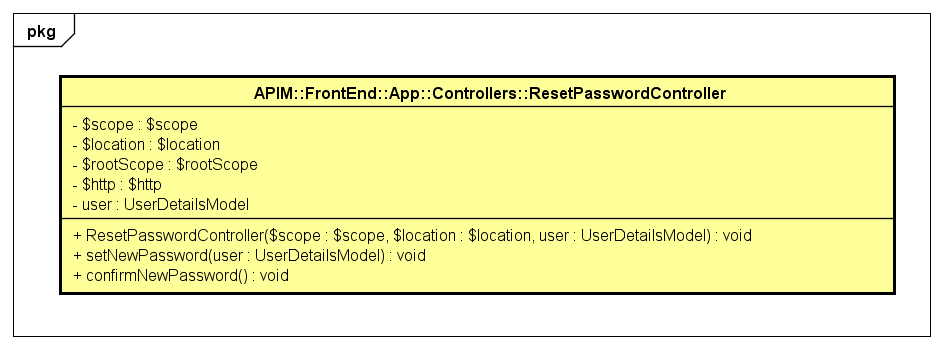
\includegraphics
	[width=0.7\linewidth]
	{images/APIM/FrontEnd/Controllers/ResetPasswordController.png}
	\caption{APIM::FrontEnd::App::Controllers::ResetPasswordController}
\end{figure}

\begin{itemize}
	\item \textbf{Descrizione:} ResetPasswordController permette di gestire il cambio password di un
utente autenticato al sistema, fornendo le funzionalità per il salvataggio di una nuova password.
	\item \textbf{Attributi:}
		\begin{itemize}
		
			\item \textbf{\$scope : \$scope}\\
			Campo dati contenente un riferimento all'oggetto \$scope creato da AngularJS, viene utilizzato come mezzo di comunicazione tra il controller e la view. Contiene gli oggetti che definiscono il model dell'applicazione;
			
			\item \textbf{\$rootScope : \$rootScope}\\
			Campo dati contenente il riferimento all'oggetto globale \$rootScope creato da AngularJS. Viene utilizzato per rendere accessibile a tutti i controllers e a tutte le views l'oggetto UserDetailsModel;
			
			\item \textbf{\$location : \$location}\\
			Campo dati contenente un riferimento al servizio creato da AngularJS che permette di accedere alla barra degli indirizzi del browser, i cambiamenti all'URL nella barra degli indirizzi si riflettono in questo oggetto e viceversa;

			\item \textbf{\$http : \$http }\\
			Campo dati che contiene un riferimento al servizio \$http che permette la comunicazione con il protocollo HTTP;
				
			\item \textbf{user : UserDetailsModel }\\
			Campo dati che si riferisce alla classe che rappresenta il modello di un utente.
				
		\end{itemize}
	\item \textbf{Metodi:}
		\begin{itemize}
		
			\item \textbf{ResetPasswordController(\$scope : \$scope, \$location : \$location, user : UserDetailsModel) : void) : void}\\
			Metodo costruttore della classe.
			\begin{description}
    			\item[\textbf{Parametri:}]
			\end{description}
			\begin{itemize}
				\item \textbf{\$scope}\\
				Parametro che contiene un riferimento all'oggetto \$scope di AngularJS, impiegato nella comunicazione tra i rispettivi view e controller. Contiene gli oggetti che definiscono i model dell'applicazione;
				
				\item \textbf{\$location}\\
				Parametro che contiene un riferimento al servizio di AngularJS che permette di accedere alla barra degli indirizzi del browser, così da controllarne i cambiamenti;
				
				\item \textbf{user}\\
				Parametro che rappresenta un utente.
			\end{itemize}
			
			\item \textbf{setNewPassword(user : UserDetailsModel) : void}\\
			Metodo per scegliere ed impostare una nuova password. Per aggiornare la nuova password, si serve di un'operazione di un servizio esposto dal package \textbf{Services}.
			\begin{description}
    			\item[\textbf{Parametri:}]
			\end{description}
			\begin{itemize}
				\item \textbf{user}\\
				Parametro che rappresenta un utente.
			\end{itemize}
			
			\item \textbf{ confirmNewPassword() : void}\\
			Metodo per confermare la nuova password. Si serve di un'operazione di un servizio esposto dal package \textbf{Services}.
			
		\end{itemize}
	\item \textbf{Relazioni con altre classi:}
		\begin{itemize}
			\item Ricava i dati necessari dal package \textbf{Services};
			\item Gestisce il funzionamento della view \textbf{ResetPassword};
			\item Il model \textbf{UsersDetailModel} che contiene le informazioni per rappresentare un utente.
		\end{itemize}
\end{itemize}

\paragraph{APIM::FrontEnd::App::Controllers::APIPurchasedController}

\begin{figure}[H]
	\centering
	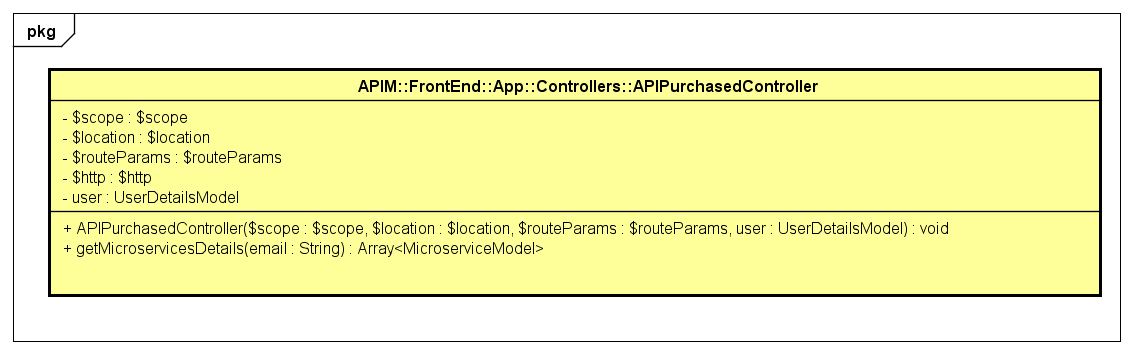
\includegraphics
	[width=0.7\linewidth]
	{images/APIM/FrontEnd/Controllers/APIPurchasedController.png}
	\caption{APIM::FrontEnd::App::Controllers::APIPurchasedController}
\end{figure}

\begin{itemize}
	\item \textbf{Descrizione:} APIPurchasedController permette di visualizzare la lista delle API comprate dall'utente ed accederne alla pagina delle informazioni dettagliate di ciascuna.
	\item \textbf{Attributi:}
		\begin{itemize}
		
			\item \textbf{\$scope : \$scope}\\
			Campo dati contenente un riferimento all'oggetto \$scope creato da AngularJS, viene utilizzato come mezzo di comunicazione tra il controller e la view. Contiene gli oggetti che definiscono il model dell'applicazione;
			
			\item \textbf{\$routeParams : \$routeParams}\\
			Parametro contenente il riferimento all'oggetto globale \$routeParams creato da AngularJS. Tale servizio permette di recuperare il set di variabili presenti nell'URL.
			
			\item \textbf{\$rootScope : \$rootScope}\\
			Campo dati contenente il riferimento all'oggetto globale \$rootScope creato da AngularJS. Viene utilizzato per rendere accessibile a tutti i controllers e a tutte le views gli oggetti MicroserviceModel e TransactionModel;
			
			\item \textbf{\$location : \$location}\\
			Campo dati contenente un riferimento al servizio creato da AngularJS che permette di accedere alla barra degli indirizzi del browser, i cambiamenti all'URL nella barra degli indirizzi si riflettono in questo oggetto e viceversa;

			\item \textbf{\$http : \$http }\\
			Campo dati che contiene un riferimento al servizio \$http che permette la comunicazione con il protocollo HTTP;
				
			\item \textbf{microservice : MicroserviceModel }\\
			Campo dati che si riferisce alla classe che rappresenta il modello di un microservizio.
			
			\item \textbf{transaction : TransactionModel }\\
			Campo dati che si riferisce alla classe che rappresenta il modello di una transazione.
				
		\end{itemize}
	\item \textbf{Metodi:}
		\begin{itemize}
		
			\item \textbf{APIPurchasedController(\$scope : \$scope, \$location : \$location, \$routeParams : \$routeParams, user : UserDetailsModel) : void}\\
			Metodo costruttore della classe.
			\begin{description}
    			\item[\textbf{Parametri:}]
			\end{description}
			\begin{itemize}
				\item \textbf{\$scope}\\
				Parametro che contiene un riferimento all'oggetto \$scope di AngularJS, impiegato nella comunicazione tra i rispettivi view e controller. Contiene gli oggetti che definiscono i model dell'applicazione;
				
				\item \textbf{\$location}\\
				Parametro che contiene un riferimento al servizio di AngularJS che permette di accedere alla barra degli indirizzi del browser, così da controllarne i cambiamenti;
			
				\item \textbf{\$routeParams}\\
				Parametro che contiene il riferimento all'oggetto globale \$routeParams di AngularJS. Permette di recuperare il set di variabili presenti nell'url;
				
				\item \textbf{user}\\
				Parametro che rappresenta un utente.
			\end{itemize}
			
			\item \textbf{getMicroservicesDetails(email : string) : Array<MicroserviceModel>}\\
			Metodo per visualizzare le informazioni dei microservizi comprati dall'utente. Si serve di un'operazione di un servizio esposto dal package \textbf{Services}.
			\begin{description}
    			\item[\textbf{Parametri:}]
			\end{description}
			\begin{itemize}
				\item \textbf{email}\\
				Parametro che rappresenta un indirizzo email.
			\end{itemize}
			
		\end{itemize}
	\item \textbf{Relazioni con altre classi:}
		\begin{itemize}
			\item Ricava i dati necessari dal package \textbf{Services};
			\item Gestisce il funzionamento della view \textbf{APIPurchased};
			\item Il model \textbf{MicroserviceModel} che contiene le informazioni per rappresentare un microservizio.
		\end{itemize}
\end{itemize}

% Fine controllers

\subsection{APIM::FrontEnd::App::node\_modules}

\subsubsection{Informazioni generali}

\begin{figure}[H]
	\centering
	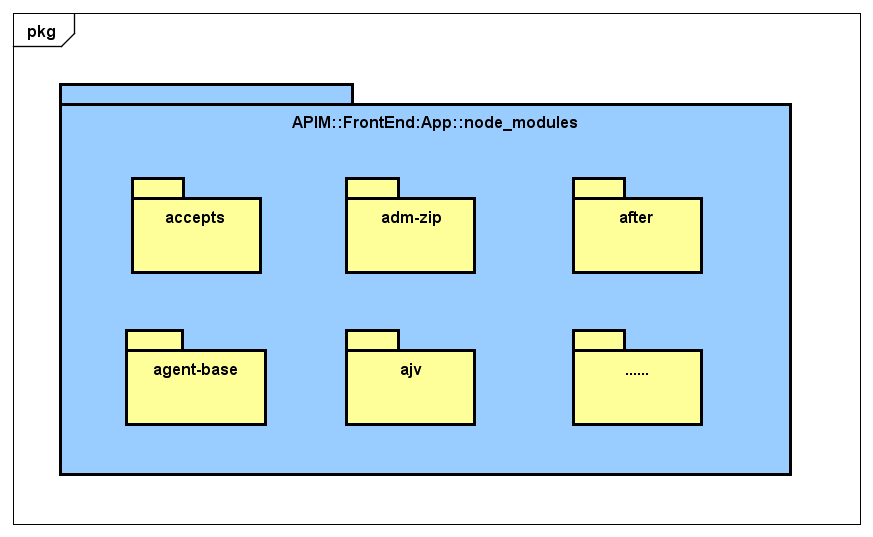
\includegraphics
	[width=0.7\linewidth]
	{images/APIM/FrontEnd/NodeModules.png}
	\caption{APIM::FrontEnd::App::node\_modules}
\end{figure}

\begin{itemize}
	\item \textbf{Descrizione:} Il package \textit{node\_modules} contiene tutti i moduli che Node.js mette a disposizione e che possono essere utilizzati dall'applicazione web.
\end{itemize}

%fine node modules
\section{Specifica Back-End}

\subsection{APIMarket::Back-End}

\subsubsection{Informazioni generali}

\begin{figure}[H]
	\centering
	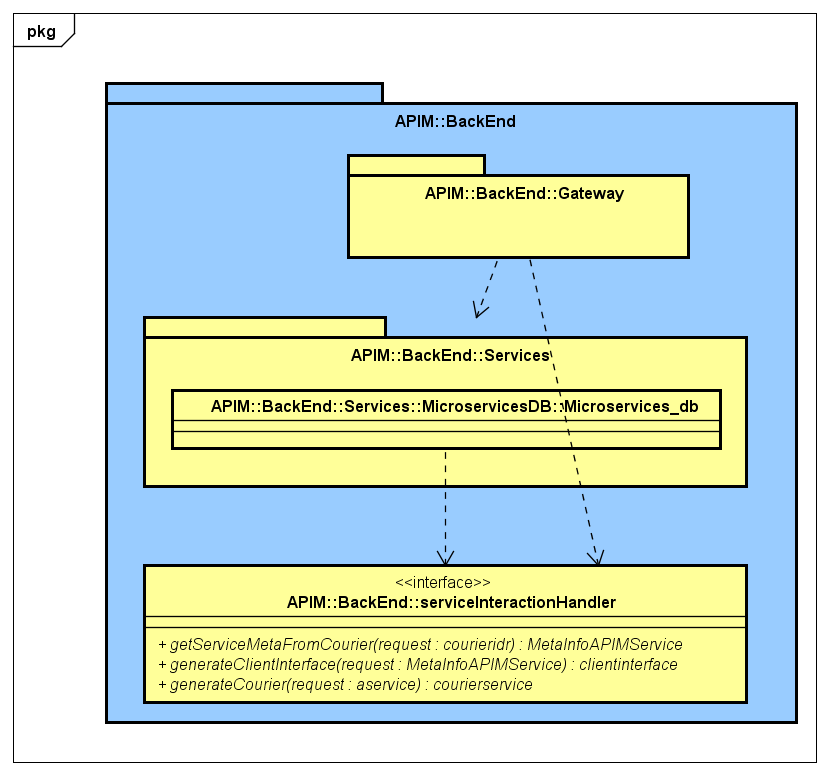
\includegraphics
	[width=0.7\linewidth]
	{UML/DiagrammiPackage/BackEnd.png}
	\caption{Package APIM::BackEnd}
\end{figure}

\begin{itemize}
	\item \textbf{Descrizione:} Il package BackEnd contiene le componenti del lato back-end dell'applicazione web.
	\item \textbf{Packages contenuti:}
	\begin{itemize}
		\item \textbf{Gateway:} package riguardante la gestione delle chiamate ai microservizi.
		\item \textbf{Services:} package riguardante la comunicazione con i database di API Market.
	\end{itemize}
\end{itemize}

\subsubsection{Interfacce}

\paragraph{ServiceInteractionHandler}
\begin{figure}[H]
	\centering
	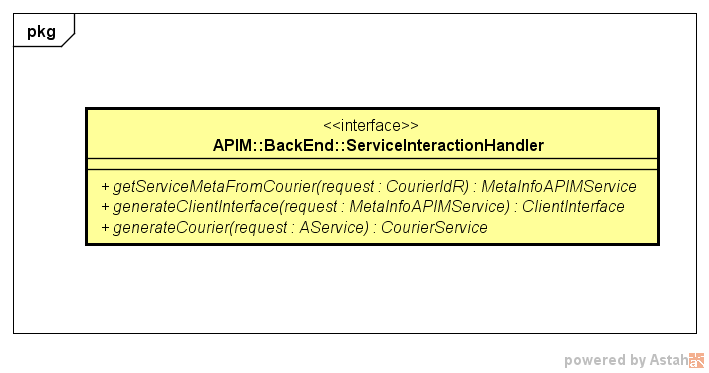
\includegraphics
	[width=0.7\linewidth]
	{images/APIM/BackEnd/Interfacce/serviceInteractionHandler.png}
	\caption{Package APIM::BackEnd::ServiceInteractionHandler}
\end{figure}

\begin{itemize}
	\item \textbf{Descrizione:} L'interfaccia ServiceInteractionHandler contiene le operazioni riguardanti la gestione delle sessioni couriers e dei metadati dei microservizi. Viene utilizzata dal Gateway e da MicroservicesDB.
\end{itemize}

\subsection{APIMarket::Back-End::Gateway}

\subsubsection{Informazioni generali}

\begin{figure}[H]
	\centering
	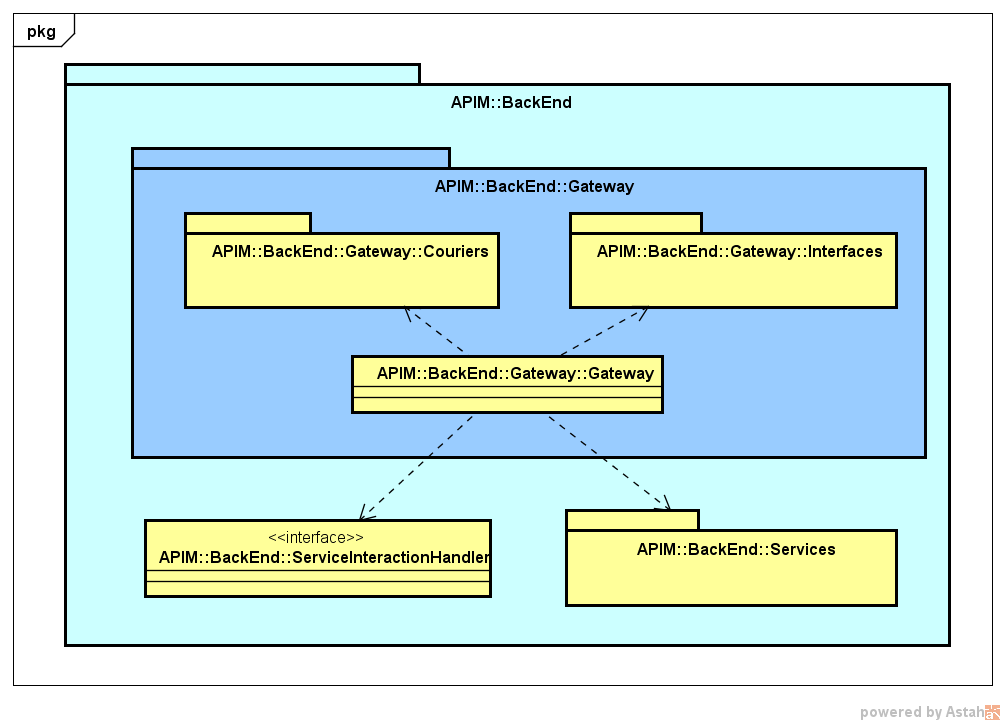
\includegraphics
	[width=0.7\linewidth]
	{UML/DiagrammiPackage/gateway.png}
	\caption{Package APIM::BackEnd::Gateway}
\end{figure}

\begin{itemize}
	\item \textbf{Descrizione:} Il package Gateway contiene le componenti del lato back-end dell'applicazione web.
	\item \textbf{Packages contenuti:}
	\begin{itemize}
		\item \textbf{Couriers:} package riguardante l'archiviazione delle sessioni couriers.
		\item \textbf{Interfaces:} package riguardante le interfacce necessarie alla classe Gateway.
	\end{itemize}
\end{itemize}

\subsubsection{Classi}

\paragraph{Gateway}
\begin{figure}[H]
	\centering
	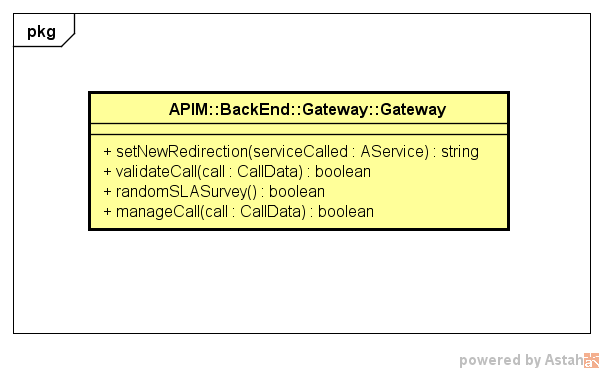
\includegraphics
	[width=0.7\linewidth]
	{images/APIM/BackEnd/Classi/gateway.png}
	\caption{Package APIM::BackEnd::Gateway::Gateway}
\end{figure}

\begin{itemize}
	\item \textbf{Descrizione:} La classe Gateway genera le sessioni courier di ciascun microservizio presente in API Market al suo avvio, ed in seguito alla registrazione di un nuovo microservizio. Inoltre si occupa della verifica della chiamata al microservizio rispetto ai dati utente ed apikey, dei rilevamenti casuali di rispetto della SLA e della loro archiviazione, della redirection verso il microservizio e l'operazione desiderati.
	\item \textbf{Relazioni:}
		\begin{itemize}
			\item La classe Gateway implementa l'interfaccia RedirectorInterface;
			\item La classe Gateway utilizza le operazioni esposte dall'interfaccia ServiceInteractionHandler;
			\item La classe Gateway utilizza le operazione esposte dalle interfacce dei servizi di comunicazione con i database, presenti nel package Services;
			\item La classe Gateway genera le sessioni courier che vengono archiviate nel package Couriers.
		\end{itemize}
	\item \textbf{Operazioni:}
		\begin{itemize}
			\item \textbf{setnewredirection( aservice )( string ):} Genera il file di courier di un microservizio e ne imposta la redirection.
				\begin{description}
    				\item[\textbf{Parametri:}]
				\end{description}
				\begin{itemize}
					\item \textbf{aservice:} Dati del microservizio dal quale generare un file courier. 
				\end{itemize}
			\item \textbf{validate\_call( calldata )( bool ):} Valida la chiamata al microservizio, verificando utente e relativa apikey. 
				\begin{description}
    				\item[\textbf{Parametri:}]
				\end{description}
				\begin{itemize}
					\item \textbf{calldata:} Dati della chiamata al microservizio.
					\item \textbf{bool}.
				\end{itemize}
			\item \textbf{random\_SLA\_survey( void )( bool ):} Algoritmo casuale per scegliere se effettuare un sondaggio della SLA.
			\item \textbf{manage\_call( calldata )( bool ):} Gestisce la chiamata al microservizio.
				\begin{description}
    				\item[\textbf{Parametri:}]
				\end{description}
				\begin{itemize}
					\item \textbf{calldata:} Dati della chiamata al microservizio.
					\item \textbf{bool}.
				\end{itemize}
		\end{itemize}
\end{itemize}

\paragraph{Redirector}
\begin{figure}[H]
	\centering
	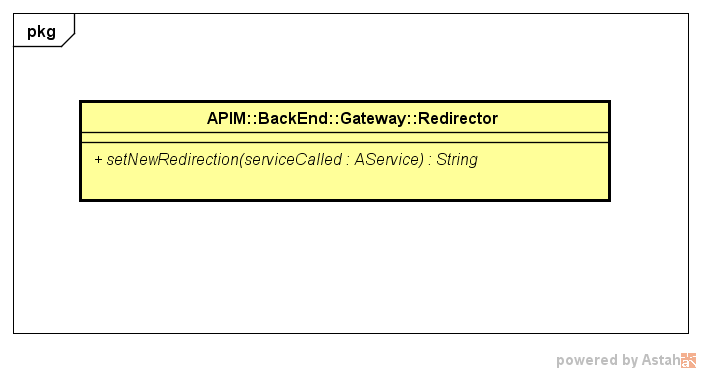
\includegraphics
	[width=0.7\linewidth]
	{images/APIM/BackEnd/Classi/redirector.png}
	\caption{Package APIM::BackEnd::Gateway::Redirector}
\end{figure}

\begin{itemize}
	\item \textbf{Descrizione:} Il package Gateway contiene le componenti del lato back-end dell'applicazione web.
	\item \textbf{Relazioni:}
	\begin{itemize}
		\item \textbf{xxxxxxx:} xxxxxxxxxxxxxxxxxxxx
		\item \textbf{xxxxxxx:} xxxxxxxxxxxxxxxxxxxx
	\end{itemize}
	\item \textbf{Operazioni:}
	\begin{itemize}
		\item \textbf{xxxxxxx:} xxxxxxxxxxxxxxxxxxxx
		\item \textbf{xxxxxxx:} xxxxxxxxxxxxxxxxxxxx
	\end{itemize}
\end{itemize}

\paragraph{ServiceInteractionHandler}
\begin{figure}[H]
	\centering
	\includegraphics
	[width=0.7\linewidth]
	{images/APIM/BackEnd/Classi/ServiceInteractionHandler.png}
	\caption{Package APIM::BackEnd::Gateway::ServiceInteractionHandler}
\end{figure}

\begin{itemize}
	\item \textbf{Descrizione:} La classe ServiceInteractionHandler implementa l'interfaccia contenuta in APIM::BackEnd::Gateway::ServiceInteractionHandlerInterface.
	\item \textbf{Relazioni:}
		\begin{itemize}
			\item La classe ServiceInteractionHandler espone le proprie operazioni alla classe Gateway;
			\item La classe ServiceInteractionHandler espone le proprie operazioni alla classe Microservices\_db.
		\end{itemize}
	\item \textbf{Operazioni:}
		\begin{itemize}
			\item \textbf{GetServiceMetaFromCourier( courierdir )( MetaInfoAPIMService ):} Ricava da una courier i metadati del servizio, cioè tipi utilizzati ed operazioni fornite.
				\begin{description}
    				\item[\textbf{Parametri:}]
				\end{description}
				\begin{itemize}
					\item \textbf{courierdir:} Directory del file courier da cui estrarre le metainfo.
					\item \textbf{MetaInfoAPIMService:} Metadati di un microservizio registrato in API Market.
				\end{itemize}
			\item \textbf{generateClientInterface( MetaInfoAPIMService )( clientinterface ):} Genera l'interfaccia esposta al client del microservizio.
				\begin{description}
    				\item[\textbf{Parametri:}]
				\end{description}
				\begin{itemize}
					\item \textbf{MetaInfoAPIMService:} Metadati di un microservizio registrato in API Market.
					\item \textbf{clientinterface:} Rappresentazione come stringa dell'interfaccia esposta al client del microservizio.
				\end{itemize}
			\item \textbf{generateCourier( aservice )( courierservice ):} Genera la rappresentazione come stringa del file courier del microservizio.
				\begin{description}
    				\item[\textbf{Parametri:}]
				\end{description}
				\begin{itemize}
					\item \textbf{aservice:} Dati del microservizio dal quale generare un file courier.
					\item \textbf{courierservice:} Rappresentazione come stringa del file courier del microservizio.
				\end{itemize}
		\end{itemize}
\end{itemize}


\subsection{APIMarket::Back-End::Gateway::GatewayInterfaces}

\subsubsection{Informazioni generali}

\begin{figure}[H]
	\centering
	\includegraphics
	[width=0.7\linewidth]
	{UML/DiagrammiPackage/gatewayinterfaces.png}
	\caption{Package APIM::BackEnd::Gateway::GatewayInterfaces}
\end{figure}

\begin{itemize}
	\item \textbf{Descrizione:} Il package GatewayInterfaces contiene le interfacce necessarie al funzionamento del Gateway. In particolare si occupa delle attività di verifica, di gestione SLA e di redirection, trattando i dati riguardanti interfaccia ed operazione della chiamata ad un microservizio.
\end{itemize}

\subsubsection{Interfacce}

\paragraph{RedirectorInterface}
\begin{figure}[H]
	\centering
	\includegraphics
	[width=0.7\linewidth]
	{images/APIM/BackEnd/Interfacce/RedirectorInterface.png}
	\caption{Package APIM::BackEnd::GatewayInterfaces/RedirectorInterface}
\end{figure}

\begin{itemize}
	\item \textbf{Descrizione:} L'interfaccia RedirectorInterface si occupa delle attività di redirection di una chiamata ad un microservizio. Sfruttando la classe ServiceInteractionHandler per generare una sessione courier, ne crea la classe Courier e le indirizza la redirection. Viene implementata dalla classe Gateway.
\end{itemize}

\subsection{APIMarket::Back-End::Services}

\subsubsection{Informazioni generali}

\begin{figure}[H]
	\centering
	\includegraphics
	[width=0.7\linewidth]
	{UML/DiagrammiPackage/services.png}
	\caption{Package APIM::BackEnd::Services}
\end{figure}

\begin{itemize}
	\item \textbf{Descrizione:} Il package Services contiene le componenti per la comunicazione con i database di API Market.
	\item \textbf{Packages contenuti:}
	\begin{itemize}
		\item \textbf{MicroservicesDB:} package riguardante la comunicazione con il database dei microservizi registrati in API Market.
		\item \textbf{UsersDB:} package riguardante la comunicazione con il database degli utenti in API Market.
		\item \textbf{TransactionsDB:} package riguardante la comunicazione con il database delle transazioni in API Market.
		\item \textbf{SLADB:} package riguardante la comunicazione con il database della SLA in API Market.
		\item \textbf{FileHandlerDB:} package riguardante la comunicazione con il database dei file in API Market.
	\end{itemize}
\end{itemize}

\subsection{APIMarket::Back-End::Services::MicroservicesDB}

\subsubsection{Informazioni generali}

\begin{figure}[H]
	\centering
	\includegraphics
	[width=0.7\linewidth]
	{UML/DiagrammiPackage/microservicesDB.png}
	\caption{Package APIM::BackEnd::Services::MicroservicesDB}
\end{figure}

\begin{itemize}
	\item \textbf{Descrizione:} Il package MicroservicesDB contiene le componenti per la comunicazione con i database dei microservizi di API Market.
\end{itemize}

\subsubsection{Interfacce}

\paragraph{MicroservicesDBInterface}
\begin{figure}[H]
	\centering
	\includegraphics
	[width=0.7\linewidth]
	{images/APIM/BackEnd/Interfacce/microservicesDBInterface.png}
	\caption{Package APIM::BackEnd::Services::MicroservicesDBInterface}
\end{figure}

\begin{itemize}
	\item \textbf{Descrizione:} L'interfaccia MicroservicesDB contiene le operazioni riguardanti lettura e scrittura dei dati dei microservizi, delle interfacce, delle categorie dei microservizi. Viene utilizzata da FrontendMS e dal Gateway.
\end{itemize}

\subsubsection{Classi}

\paragraph{MicroservicesDB}
\begin{figure}[H]
	\centering
	\includegraphics
	[width=0.7\linewidth]
	{images/APIM/BackEnd/Classi/microservicesDB.png}
	\caption{Package APIM::BackEnd::Services::MicroservicesDB}
\end{figure}

\begin{itemize}
	\item \textbf{Descrizione:} La classe MicroservicesDB implementa l'interfaccia contenuta in APIM::BackEnd::Services::Microservices\_dbInterface.
	\item \textbf{Relazioni:}
		\begin{itemize}
			\item La classe MicroservicesDB implementa l'interfaccia MicroservicesDBInterface;
			\item La classe MicroservicesDB utilizza le operazioni esposte dall'interfaccia ServiceInteractionHandlerInterface;
			\item La classe MicroservicesDB espone le proprie operazioni alla classe FrontendMS.
		\end{itemize}
	\item \textbf{Operazioni:}
		\begin{itemize}
		
			\item \textbf{retrieve\_all\_ms\_info( void )( listservices ):} Ricava le informazioni di ogni microservizio registrato in API Market.
				\begin{description}
    				\item[\textbf{Parametri:}]
				\end{description}
				\begin{itemize}
					\item \textbf{listservices:} Lista dei microservizi con relative informazioni.
				\end{itemize}
				
			\item \textbf{retrieve\_ms\_info( msid )( msdata ):} Ricava le informazioni del microservizio a partire dal suo id.
				\begin{description}
    				\item[\textbf{Parametri:}]
				\end{description}
				\begin{itemize}
					\item \textbf{msid:} Id del microservizio.
					\item \textbf{msdata:} Informazioni del microservizio.
				\end{itemize}
				
			\item \textbf{retrieve\_intf\_info( intfid )( intfdata ):} Ricava le informazioni dell'interfaccia a partire dal suo id.
				\begin{description}
    				\item[\textbf{Parametri:}]
				\end{description}
				\begin{itemize}
					\item \textbf{intfid:} Id dell'interfaccia.
					\item \textbf{intfdata:} Informazioni dell'interfaccia.
				\end{itemize}
				
			\item \textbf{retrieve\_interfaces\_of\_ms( msid )( intfidlist ):} Ricava gli id delle interfacce di un microservizio, a partire dal suo id.
				\begin{description}
    				\item[\textbf{Parametri:}]
				\end{description}
				\begin{itemize}
					\item \textbf{msid:} Id del microservizio.
					\item \textbf{intfidlist:} Lista degli id delle interfacce del microservizio.
				\end{itemize}
				
			\item \textbf{retrieve\_ms\_from\_interface( intfid )( msiddata ):} Ricava l'id del microservizio, a partire dall'id di una sua interfaccia.
				\begin{description}
    				\item[\textbf{Parametri:}]
				\end{description}
				\begin{itemize}
					\item \textbf{intfid:} Id dell'interfaccia.
					\item \textbf{msiddata:} Id del microservizio.
				\end{itemize}
				
			\item \textbf{retrieve\_msidlist\_from\_category( categoryid )( msidbycatlist ):} Ricava gli id dei microservizi appartenenti ad una categoria, a partire dall'id della categoria.
				\begin{description}
    				\item[\textbf{Parametri:}]
				\end{description}
				\begin{itemize}
					\item \textbf{categoryid:} Id della categoria.
					\item \textbf{msidbycatlist:} Lista degli id dei microservizi appartenenti alla categoria.
				\end{itemize}
				
			\item \textbf{retrieve\_category\_info( categoryid )( categorydata ):} Ricava le informazioni di una categoria, a partire dal suo id.
				\begin{description}
    				\item[\textbf{Parametri:}]
				\end{description}
				\begin{itemize}
					\item \textbf{categoryid:} Id della categoria.
					\item \textbf{categorydata:} Informazioni della categoria.
				\end{itemize}
				
			\item \textbf{retrieve\_categories\_of\_ms( msid )( categoryidlist ):} Ricava gli id delle categorie attribuite al microservizio, a partire dall'id del microservizio.
				\begin{description}
    				\item[\textbf{Parametri:}]
				\end{description}
				\begin{itemize}
					\item \textbf{msid:} Id del microservizio.
					\item \textbf{categoryidlist:} Lista degli id delle categorie attribuite al microservizio.
				\end{itemize}
				
			\item \textbf{retrieve\_last\_registered\_ms( shownumber )( lastmsreglist ):} Ricava un numero specificato dei microservizi registrati più recentemente su API Market.
				\begin{description}
    				\item[\textbf{Parametri:}]
				\end{description}
				\begin{itemize}
					\item \textbf{shownumber:} La lunghezza della lista massima dei microservizi registrati più recentemente su API Market.
					\item \textbf{lastmsreglist:} La lista dei microservizi registrati più recentemente su API Market con relative informazioni.
				\end{itemize}
				
			\item \textbf{retrieve\_last\_registered\_ms\_info( idms )( lastmsregbyidlist ):} Ricava Nome, IdDeveloper e Logo del microservizio, a partire dal suo id.
				\begin{description}
    				\item[\textbf{Parametri:}]
				\end{description}
				\begin{itemize}
					\item \textbf{msid:} Id del microservizio.
					\item \textbf{lastmsregbyidlist:} Name, IdDeveloper e Logo del microservizio.
				\end{itemize}
				
			\item \textbf{microservice\_registration( msdataw )( bool ):} Registra un nuovo microservizio nel database dei microservizi.
				\begin{description}
    				\item[\textbf{Parametri:}]
				\end{description}
				\begin{itemize}
					\item \textbf{msdataw:} Informazioni del nuovo microservizio.
					\item \textbf{bool}.
				\end{itemize}
				
			\item \textbf{microservice\_update( msupdata )( bool ):} Aggiorna le informazioni di un microservizio esistente nel database dei microservizi.
				\begin{description}
    				\item[\textbf{Parametri:}]
				\end{description}
				\begin{itemize}
					\item \textbf{msupdata:} Informazioni aggiornate di un microservizio esistente.
					\item \textbf{bool}.
				\end{itemize}
				
			\item \textbf{interface\_registration( intfdataw )( bool ):} Registra una nuova interfaccia di un microservizio esistente nel database dei microservizi .
				\begin{description}
    				\item[\textbf{Parametri:}]
				\end{description}
				\begin{itemize}
					\item \textbf{intfdataw:} Informazioni della nuova interfaccia.
					\item \textbf{bool}.
				\end{itemize}
				
			\item \textbf{interface\_update( intfupdata )( bool):} Aggiorna le informazioni di una interfaccia esistente nel database dei microservizi.
				\begin{description}
    				\item[\textbf{Parametri:}]
				\end{description}
				\begin{itemize}
					\item \textbf{intfupdata:} Informazioni aggiornate di una interfaccia esistente.
					\item \textbf{bool}.
				\end{itemize}
				
			\item \textbf{add\_category\_to\_ms( categorydataw )( bool ):} Attribuisce una categoria ad un microservizio.
				\begin{description}
    				\item[\textbf{Parametri:}]
				\end{description}
				\begin{itemize}
					\item \textbf{categorydataw:} Id del microservizio e della categoria da attribuirgli.
					\item \textbf{bool}.
				\end{itemize}
				
			\item \textbf{remove\_category\_from\_ms( categorydataw )( bool ):} Rimuove una categoria da un microservizio.
				\begin{description}
    				\item[\textbf{Parametri:}]
				\end{description}
				\begin{itemize}
					\item \textbf{categorydataw:} Id del microservizio e della categoria da rimuovergli.
					\item \textbf{bool}.
				\end{itemize}
	
		\end{itemize}
\end{itemize}

\subsection{APIMarket::Back-End::Services::UsersDB}

\subsubsection{Informazioni generali}

\begin{figure}[H]
	\centering
	\includegraphics
	[width=0.7\linewidth]
	{UML/DiagrammiPackage/usersDB.png}
	\caption{Package APIM::BackEnd::Services::UsersDB}
\end{figure}

\begin{itemize}
	\item \textbf{Descrizione:} Il package \textit{UsersDB} contiene le componenti per la comunicazione con il database degli utenti di API Market.
\end{itemize}

\subsubsection{Interfacce}

\paragraph{UsersDBInterface}
\begin{figure}[H]
	\centering
	\includegraphics
	[width=0.7\linewidth]
	{images/APIM/BackEnd/Interfacce/usersDBInterface.png}
	\caption{Package APIM::BackEnd::Services::UsersDBInterface}
\end{figure}

\begin{itemize}
	\item \textbf{Descrizione:} L'interfaccia UsersDBInterface contiene le operazioni riguardanti lettura e scrittura dei dati degli utenti (sia admin che clienti), dei tipi di cliente, delle moderazioni attuate, dei tipi di moderazione. Viene utilizzata da FrontendMS e dal Gateway.
\end{itemize}

\subsubsection{Classi}

\paragraph{UsersDB}
\begin{figure}[H]
	\centering
	\includegraphics
	[width=0.7\linewidth]
	{images/APIM/BackEnd/Classi/usersDB.png}
	\caption{Package APIM::BackEnd::Services::UsersDB}
\end{figure}

\begin{itemize}
	\item \textbf{Descrizione:} La classe UsersDB implementa l'interfaccia contenuta in APIM::BackEnd::Services::Users\_dbInterface.
	\item \textbf{Relazioni:}
		\begin{itemize}
			\item La classe UsersDB implementa l'interfaccia UsersDBInterface;
			\item La classe UsersDB espone le proprie operazioni alla classe FrontendMS.
		\end{itemize}
	\item \textbf{Operazioni:}
		\begin{itemize}
		
			\item \textbf{user\_exists( logininfo )( bool ):} Controlla se il cliente esista nel database utenti.
				\begin{description}
    				\item[\textbf{Parametri:}]
				\end{description}
				\begin{itemize}
					\item \textbf{logininfo:} Email ed Password del cliente.
					\item \textbf{bool}.
				\end{itemize}
				
			\item \textbf{retrieve\_admin\_info( adminid )( admindata ):} Ricava le informazioni dell'admin, a partire dal suo id.
				\begin{description}
    				\item[\textbf{Parametri:}]
				\end{description}
				\begin{itemize}
					\item \textbf{adminid:} Id dell'admin.
					\item \textbf{admindata:} Informazioni dell'admin.
				\end{itemize}
				
			\item \textbf{retrieve\_client\_info( clientid )( clientdata ):} Ricava le informazioni del cliente, a partire dal suo id.
				\begin{description}
    				\item[\textbf{Parametri:}]
				\end{description}
				\begin{itemize}
					\item \textbf{clientid:} Id del cliente.
					\item \textbf{clientdata:} Informazioni del cliente.
				\end{itemize}
				
			\item \textbf{retrieve\_client\_fullname( clientid )( clientfullnamedata ):} Ricava Name e Surname del client, a partire dal suo id.
				\begin{description}
    				\item[\textbf{Parametri:}]
				\end{description}
				\begin{itemize}
					\item \textbf{clientid:} Id del cliente.
					\item \textbf{clientfullnamedata:} Name e Surname del cliente.
				\end{itemize}
				
			\item \textbf{retrieve\_client\_type( clientid )( typeiddata ):} Ricava il tipo di account del cliente, a partire dal suo id.
				\begin{description}
    				\item[\textbf{Parametri:}]
				\end{description}
				\begin{itemize}
					\item \textbf{clientid:} Id del cliente.
					\item \textbf{typeiddata:} Id del tipo di account del cliente.
				\end{itemize}
			
			\item \textbf{retrieve\_moderation\_info( modentryid )( entrydata ):} Ricava le informazioni della moderazione, a partire dal suo id.
				\begin{description}
    				\item[\textbf{Parametri:}]
				\end{description}
				\begin{itemize}
					\item \textbf{modentryid:} Id della moderazione.
					\item \textbf{entrydata:} Informazioni della moderazione.
				\end{itemize}
				
			\item \textbf{retrieve\_modtype\_info( modtypeid )( modtypedata ):} Ricava le informazioni del tipo di moderazione, a partire dal suo id.
				\begin{description}
    				\item[\textbf{Parametri:}]
				\end{description}
				\begin{itemize}
					\item \textbf{modtypeid:} Id del tipo di moderazione.
					\item \textbf{modtypedata:} Informazioni del tipo di moderazione.
				\end{itemize}
				
			\item \textbf{retrieve\_clienttype\_info( clienttypeid )( clienttypedata ):} Ricava le informazioni del tipo di account del cliente, a partire dal suo id.
				\begin{description}
    				\item[\textbf{Parametri:}]
				\end{description}
				\begin{itemize}
					\item \textbf{clienttypeid:} Id del tipo di account del cliente.
					\item \textbf{clienttypedata:} Informazioni del tipo di account del cliente.
				\end{itemize}
				
			\item \textbf{basicclient\_registration( basicclientdata )( bool ):} Registra un nuovo account cliente di tipo base.
				\begin{description}
    				\item[\textbf{Parametri:}]
				\end{description}
				\begin{itemize}
					\item \textbf{basicclientdata:} Informazioni del nuovo cliente.
					\item \textbf{bool}.
				\end{itemize}
				
			\item \textbf{developer\_upgrade( developerdata )( bool ):} Effettua l'upgrade ad account sviluppatore di un cliente.
				\begin{description}
    				\item[\textbf{Parametri:}]
				\end{description}
				\begin{itemize}
					\item \textbf{developerdata:} Informazioni dei campi aggiuntivi da sviluppatore.
					\item \textbf{bool}.
				\end{itemize}
				
			\item \textbf{basicclient\_downgrade( clientid )( bool ):} Effettua il downgrade ad account base di un cliente sviluppatore.
				\begin{description}
    				\item[\textbf{Parametri:}]
				\end{description}
				\begin{itemize}
					\item \textbf{clientid:} Id del cliente.
					\item \textbf{bool}.
				\end{itemize}
				
			\item \textbf{client\_moderation( entrydataw )( bool ):} Inserisce una nuova moderazione nel database degli utenti.
				\begin{description}
    				\item[\textbf{Parametri:}]
				\end{description}
				\begin{itemize}
					\item \textbf{entrydataw:} Informazioni della nuova moderazione.
					\item \textbf{bool}.
				\end{itemize}
				
			\item \textbf{client\_update( userdata )( bool ):} Aggiorna le informazioni di un cliente.
				\begin{description}
    				\item[\textbf{Parametri:}]
				\end{description}
				\begin{itemize}
					\item \textbf{userdata:} Informazioni aggiornate del cliente.
					\item \textbf{bool}.
				\end{itemize}
				
			\item \textbf{client\_delete( clientid )( bool ):} Elimina un cliente da API Market.
				\begin{description}
    				\item[\textbf{Parametri:}]
				\end{description}
				\begin{itemize}
					\item \textbf{clientid:} Id del cliente.
					\item \textbf{bool}.
				\end{itemize}
					
		\end{itemize}
\end{itemize}

\subsection{APIMarket::Back-End::Services::TransactionsDB}

\subsubsection{Informazioni generali}

\begin{figure}[H]
	\centering
	\includegraphics
	[width=0.7\linewidth]
	{UML/DiagrammiPackage/transactionsDB.png}
	\caption{Package APIM::BackEnd::Services::TransactionsDB}
\end{figure}

\begin{itemize}
	\item \textbf{Descrizione:} Il package \textit{TransactionsDB} contiene le componenti per la comunicazione con il database delle transazioni di API Market.
\end{itemize}

\subsubsection{Interfacce}

\paragraph{TransactionsDBInterface}
\begin{figure}[H]
	\centering
	\includegraphics
	[width=0.7\linewidth]
	{images/APIM/BackEnd/Interfacce/transactionsDBInterface.png}
	\caption{Package APIM::BackEnd::Services::TransactionsDBInterface}
\end{figure}

\begin{itemize}
	\item \textbf{Descrizione:} L'interfaccia Transactions\_dbInterface contiene le operazioni riguardanti lettura e scrittura dei dati delle apikey, degli acquisti. Viene utilizzata da FrontendMS e dal Gateway.
\end{itemize}

\subsubsection{Classi}

\paragraph{TransactionsDB}
\begin{figure}[H]
	\centering
	\includegraphics
	[width=0.7\linewidth]
	{images/APIM/BackEnd/Classi/transactionsDB.png}
	\caption{Package APIM::BackEnd::Services::TransactionsDB}
\end{figure}

\begin{itemize}
	\item \textbf{Descrizione:} La classe Transactions\_db implementa l'interfaccia contenuta in APIM::BackEnd::Services::TransactionsDBInterface.
	\item \textbf{Relazioni:}
		\begin{itemize}
			\item La classe TransactionsDB implementa l'interfaccia TransactionsDBInterface;
			\item La classe TransactionsDB espone le proprie operazioni alla classe FrontendMS.
		\end{itemize}
	\item \textbf{Operazioni:}
		\begin{itemize}
		
			\item \textbf{retrieve\_apikey\_info( apikeyid )( apikey ):} Ricava le informazioni dell'apikey, a partire dal suo id.
				\begin{description}
    				\item[\textbf{Parametri:}]
				\end{description}
				\begin{itemize}
					\item \textbf{apikeyid:} Id dell'apikey.
					\item \textbf{apikey:} Informazioni dell'apikey.
				\end{itemize}
				
			\item \textbf{retrieve\_purchases\_list( clientid )( purchaseslist ):} Ricava la lista con relative informazioni delle transazioni del cliente, a partire dal suo id.
				\begin{description}
    				\item[\textbf{Parametri:}]
				\end{description}
				\begin{itemize}
					\item \textbf{clientid:} Id del cliente.
					\item \textbf{purchaseslist:} Lista delle transazioni del cliente con relative informazioni.
				\end{itemize}
				
			\item \textbf{apikey\_registration( apikeydataw )( bool ):} Registra una nuova apikey nel database delle transazioni.
				\begin{description}
    				\item[\textbf{Parametri:}]
				\end{description}
				\begin{itemize}
					\item \textbf{apikeydataw:} Informazioni della nuova apikey.
					\item \textbf{bool}.
				\end{itemize}
				
			\item \textbf{purchase\_registration( purchasedata )( bool ):} Inserisce una nuova transazione nel database delle transazioni.
				\begin{description}
    				\item[\textbf{Parametri:}]
				\end{description}
				\begin{itemize}
					\item \textbf{purchasedata:} Informazioni della nuova transazione.
					\item \textbf{bool}.
				\end{itemize}
				
			\item \textbf{apikey\_remaining\_update( apikeyremainingdata )( bool ):} Aggiorna il Remaining della apikey, a partire dal suo id e dal valore del cambiamento.
				\begin{description}
    				\item[\textbf{Parametri:}]
				\end{description}
				\begin{itemize}
					\item \textbf{apikeyremainingdata:} Id dell'apikey e valore del cambiamento.
					\item \textbf{bool}.
				\end{itemize}
				
		\end{itemize}
\end{itemize}

\subsection{APIMarket::Back-End::Services::SLADB}

\subsubsection{Informazioni generali}

\begin{figure}[H]
	\centering
	\includegraphics
	[width=0.7\linewidth]
	{UML/DiagrammiPackage/SLADB.png}
	\caption{Package APIM::BackEnd::Services::SLADB}
\end{figure}

\begin{itemize}
	\item \textbf{Descrizione:} Il package \textit{SLADB} contiene le componenti per la comunicazione con il database della SLA di API Market.
\end{itemize}

\subsubsection{Interfacce}

\paragraph{SlaDBInterface}
\begin{figure}[H]
	\centering
	\includegraphics
	[width=0.7\linewidth]
	{images/APIM/BackEnd/Interfacce/slaDBInterface.png}
	\caption{Package APIM::BackEnd::Services::SlaDBInterface}
\end{figure}

\begin{itemize}
	\item \textbf{Descrizione:} L'interfaccia Sla\_dbInterface contiene le operazioni riguardanti lettura e scrittura dei dati dei sondaggi SLA. Viene utilizzata da FrontendMS e dal Gateway.
\end{itemize}

\subsubsection{Classi}

\paragraph{Sla\_db}
\begin{figure}[H]
	\centering
	\includegraphics
	[width=0.7\linewidth]
	{images/APIM/BackEnd/Classi/slaDB.png}
	\caption{Package APIM::BackEnd::Services::SlaDB}
\end{figure}

\begin{itemize}
	\item \textbf{Descrizione:} La classe SlaDB implementa l'interfaccia contenuta in APIM::BackEnd::Services::SlaDBInterface.
	\item \textbf{Relazioni:}
		\begin{itemize}
			\item La classe SlaDB implementa l'interfaccia SlaDBInterface;
			\item La classe SlaDB espone le proprie operazioni alla classe FrontendMS.
		\end{itemize}
	\item \textbf{Operazioni:}
		\begin{itemize}
		
			\item \textbf{retrieve\_apikey\_slasurvey\_list( apikeyid )( slasurveylist ):} Ricava la lista dei sondaggi SLA dell'apikey con relative informazioni, a partire dall'id dell'apikey.
				\begin{description}
    				\item[\textbf{Parametri:}]
				\end{description}
				\begin{itemize}
					\item \textbf{apikeyid:} Id dell'apikey.
					\item \textbf{slasurveylist:} Lista dei sondaggi SLA con relative informazioni.
				\end{itemize}
				
			\item \textbf{retrieve\_ms\_slasurvey\_list( msid )( slasurveylistms ):} Ricava la lista dei sondaggi SLA del microservizio con relative informazioni, a partire dall'id del microservizio.
				\begin{description}
    				\item[\textbf{Parametri:}]
				\end{description}
				\begin{itemize}
					\item \textbf{msid:} Id del microservizio.
					\item \textbf{slasurveylistms:} Lista dei sondaggi SLA con relative informazioni.
				\end{itemize}
				
			\item \textbf{retrieve\_slasurvey\_info( slasurveyid )( slasurvey ):} Ricava le informazioni del sondaggio SLA, a partire dal suo id.
				\begin{description}
    				\item[\textbf{Parametri:}]
				\end{description}
				\begin{itemize}
					\item \textbf{slasurveyid:} Id del sondaggio SLA.
					\item \textbf{slasurvey:} Informazioni del sondaggio SLA.
				\end{itemize}
				
			\item \textbf{retrieve\_slasurvey\_iscompliant( slasurveyid )( bool ):} Ricava IsCompliant del sondaggio SLA, a partire dal suo id.
				\begin{description}
    				\item[\textbf{Parametri:}]
				\end{description}
				\begin{itemize}
					\item \textbf{slasurveyid:} Id del sondaggio SLA.
					\item \textbf{bool}.
				\end{itemize}
				
			\item \textbf{slasurvey\_insert( slasurveydataw )( bool ):} Inserisce un nuovo sondaggio SLA nel database della SLA.
				\begin{description}
    				\item[\textbf{Parametri:}]
				\end{description}
				\begin{itemize}
					\item \textbf{slasurveydataw:} Informazioni del nuovo sondaggio SLA.
					\item \textbf{bool}.
				\end{itemize}
				
		\end{itemize}
\end{itemize}

\subsection{APIMarket::Back-End::Services::FilehandlerDB}

\subsubsection{Informazioni generali}

\begin{figure}[H]
	\centering
	\includegraphics
	[width=0.7\linewidth]
	{UML/DiagrammiPackage/filehandlerDB.png}
	\caption{Package APIM::BackEnd::Services::FilehandlerDB}
\end{figure}

\begin{itemize}
	\item \textbf{Descrizione:} Il package FilehandlerDB contiene le componenti per la comunicazione con il database dei file di API Market.
\end{itemize}

\subsubsection{Interfacce}

\paragraph{FilehandlerInterface}
\begin{figure}[H]
	\centering
	\includegraphics
	[width=0.7\linewidth]
	{images/APIM/BackEnd/Interfacce/fileHandlerInterface.png}
	\caption{Package APIM::BackEnd::Services::FilehandlerDB::FilehandlerInterface}
\end{figure}

\begin{itemize}
	\item \textbf{Descrizione:} L'interfaccia FilehandlerDBInterface contiene le operazioni riguardanti lettura e scrittura dei dati dei file. Viene utilizzata da FrontendMS e dal Gateway.
\end{itemize}

\subsubsection{Classi}

\paragraph{FilehandlerDB}
\begin{figure}[H]
	\centering
	\includegraphics
	[width=0.7\linewidth]
	{images/APIM/BackEnd/Classi/fileHandler.png}
	\caption{Package APIM::BackEnd::Services::FilehandlerDB::Filehandler}
\end{figure}

\begin{itemize}
	\item \textbf{Descrizione:} La classe Filehandler implementa l'interfaccia contenuta in APIM::BackEnd::Services::Filehandler\_dbInterface.
	\item \textbf{Relazioni:}
		\begin{itemize}
			\item La classe FilehandlerDB implementa l'interfaccia FilehandlerDBInterface;
		\end{itemize}
	\item \textbf{Operazioni:}
		\begin{itemize}
		
			\item \textbf{setFile( SetFileRequest )( string ):} Archivia il file, se non è già presente nell'archivio, salvandolo con un nome univoco e ricava l'uri corrispondente.
				\begin{description}
    				\item[\textbf{Parametri:}]
				\end{description}
				\begin{itemize}
					\item \textbf{SetFileRequest:} Informazioni del file.
					\item \textbf{string}.
				\end{itemize}
				
			\item \textbf{filenameExists( string )( bool ):} Controlla se nel database dei file esista un file con il nome specificato.
				\begin{description}
    				\item[\textbf{Parametri:}]
				\end{description}
				\begin{itemize}
					\item \textbf{string}.
					\item \textbf{bool}.
				\end{itemize}
				
		\end{itemize}
\end{itemize}
\newpage
\section{Diagrammi di sequenza}

\subsection{Front-End}
I seguenti diagrammi di sequenza prendono in considerazione le principali operazioni del front-end e vanno ad illustrarne le interazioni tra le classi.

\subsubsection{Registrazione utente}

\begin{figure}[H]
	\centering
	\includegraphics
	[width=0.7\linewidth]
	{UML/DiagrammiSequenza/registrazione_utente.png}
	\caption{Diagramma di sequenza: Registrazione utente}
\end{figure}

\begin{itemize}
	\item \textbf{Pre-condizioni}: l'utente si trova nella schermata di registrazione utente;
	\item \textbf{Post-condizioni}: l'utente ha compilato il form per la registrazione ed ora possiede le credenziali per l'autenticazione alla piattaforma API Market;
	\item \textbf{Descrizione}: l'utente compila il form per la registrazione di un account, provvedendo ad inserire tutte le informazioni obbligatorie richieste. Confermando la registrazione, i services di API Market provvedono ad inserire nel database il nuovo utente. A registrazione avvenuta, l'utente riceve un messaggio di successo e viene reindirizzato alla pagina di login.
\end{itemize}


\subsubsection{Autenticazione}

\begin{figure}[H]
	\centering
	\includegraphics
	[width=0.7\linewidth]
	{UML/DiagrammiSequenza/login.png}
	\caption{Diagramma di sequenza: Autenticazione}
\end{figure}

\begin{itemize}
	\item \textbf{Pre-condizioni}: l'utente si trova nella schermata di autenticazione;
	\item \textbf{Post-condizioni}: l'utente ha compilato il form per il login ed ora risulta un utente autenticato al sistema API Market;
	\item \textbf{Descrizione}: l'utente compila il form per l'autenticazione, provvedendo ad inserire la propria email e password con le quali si era registrato. Confermando l'autenticazione, la piattaforma API Market provvede a creare una sessione per l'utente autenticato, il quale, nel caso di autenticazione avvenuta con successo, viene reindirizzato alla home dell'applicazione.
\end{itemize}
\clearpage

\subsubsection{Recupero password}

\begin{figure}[H]
	\centering
	\includegraphics
	[width=0.7\linewidth]
	{UML/DiagrammiSequenza/recupero_password.png}
	\caption{Diagramma di sequenza: Recupero password}
\end{figure}

\begin{itemize}
	\item \textbf{Pre-condizioni}: l'utente si trova nella schermata di recupero password;
	\item \textbf{Post-condizioni}: l'utente ha compilato il form per il recupero della propria password tramite email ed ora può ri-effettuare l'autenticazione alla piattaforma API Market;
	\item \textbf{Descrizione}: l'utente compila il form per il recupero della password relativa al proprio account, inserendo l'email dove il sistema inoltrerà la nuova password generata. Confermando l'operazione, i services di API Market provvedono ad aggiornare il campo password nel database degli utenti. A recupero avvenuto, l'utente riceve un messaggio di successo e viene reindirizzato alla pagina di login.
\end{itemize}
\clearpage

\subsubsection{Ricerca API}

\begin{figure}[H]
	\centering
	\includegraphics
	[width=0.7\linewidth]
	{UML/DiagrammiSequenza/ricercaAPI.png}
	\caption{Diagramma di sequenza: Ricerca API}
\end{figure}

\begin{itemize}
	\item \textbf{Pre-condizioni}: l'utente si trova nella homepage dell'applicazione;
	\item \textbf{Post-condizioni}: l'utente ha visualizzato le API secondo la categoria e le keywords inserite;
	\item \textbf{Descrizione}: di default, la homepage di API Market mostra le API registrate più recentemente. L'utente può immettere delle keywords nell'apposito riquadro per alterare i risultati, e scegliere di restringere la ricerca ad una singola categoria. I risultati visualizzati cambiano dinamicamente non appena l'applicazione web riceve risposta dai servizi che la collegano ai database.
\end{itemize}
\clearpage

\subsubsection{Acquisto API}

\begin{figure}[H]
	\centering
	\includegraphics
	[width=0.7\linewidth]
	{UML/DiagrammiSequenza/acquistoAPI.png}
	\caption{Diagramma di sequenza: Acquisto API}
\end{figure}

\begin{itemize}
	\item \textbf{Pre-condizioni}: il cliente si trova nella schermata di acquisto di una specifica API;
	\item \textbf{Post-condizioni}: il cliente ha ricevuto l'API Key per l'API acquistata, secondo le modalità da lui scelte, e gli sono stati sottratti i corrispondenti crediti;
	\item \textbf{Descrizione}: il cliente compila il form per l'acquisto dell'API desiderata, visualizzando il preventivo di crediti spesi in base ai parametri scelti. Confermando l'acquisto (che può essere anche un rinnovo), i services di API Market provvedono a generare una apikey ed a scalare i crediti dall'account utente. L'utente potrà visualizzare l'API Key ed un messaggio di ringraziamento.
\end{itemize}
\clearpage

\subsubsection{Inserimento API}

\begin{figure}[H]
	\centering
	\includegraphics
	[width=0.7\linewidth]
	{UML/DiagrammiSequenza/registrazioneAPI.png}
	\caption{Diagramma di sequenza: Inserimento API}
\end{figure}

\begin{itemize}
	\item \textbf{Pre-condizioni}: lo sviluppatore si trova nella schermata di registrazione di una nuova API;
	\item \textbf{Post-condizioni}: lo sviluppatore ha registrato la sua nuova API ed essa è ora disponibile in API Market;
	\item \textbf{Descrizione}: lo sviluppatore compila il form per la registrazione di una nuova API, provvedendo anche a caricare sul server di API Market i file del logo e della documentazione PDF. Confermando la registrazione, i services di API Market provvedono ad inserire nel database la nuova API e renderla accessibile attraverso il Gateway. A registrazione avvenuta, lo sviluppatore riceve un messaggio di successo.
\end{itemize}
\clearpage

\subsubsection{Ricarica saldo conto virtuale}

\begin{figure}[H]
	\centering
	\includegraphics
	[width=0.7\linewidth]
	{UML/DiagrammiSequenza/ricaricaCrediti.png}
	\caption{Diagramma di sequenza: Ricarica saldo conto virtuale}
\end{figure}

\begin{itemize}
	\item \textbf{Pre-condizioni}: il cliente si trova nella schermata di ricarica del proprio conto virtuale;
	\item \textbf{Post-condizioni}: il cliente ha effettuato la ricarica dei propri crediti;
	\item \textbf{Descrizione}: il cliente stabilisce l'ammontare dei crediti da ricaricare nel proprio conto virtuale. A decisione avvenuta, verrà reindirizzato alla procedura di acquisto di PayPal, che lo guiderà nell'acquisto. Portata a termine la transazione, PayPal avvertirà i services di API Market che si occuperanno di incrementare i crediti del conto virtuale del cliente.
\end{itemize}


%\subsection{Back-End}
%I seguenti diagrammi di sequenza prendono in considerazione le principali operazioni del back-end e vanno ad illustrarne le interazioni tra le classi.

%\newpage
\renewcommand*{\arraystretch}{1.6}

\section{Tracciamento componenti}
\textbf{N.B.}: il tracciamento Componenti-Requisiti del package \textit{APIGateway} è stato omesso, in quanto esso si occupa della chiamate ai microservizi, che sono estranei alla nostra responsabilità.

\subsection{Tracciamento componenti-requisiti}
		\begin{longtable}{ p{12cm} | p{4cm} }
			\hline \rowcolor{Gray}
			\textbf{Nome Componente} & \textbf{Codice Requisito} \\
			\hline
			APIM::FrontEnd
			& RFO1 \\
			& RFO1.1 \\
			& RFO1.2 \\
			& RFO1.3 \\
			& RFO1.4 \\
			& RFO1.5 \\
			& RFO1.6 \\
			& RFO1.7 \\
			& RFO1.8 \\
			& RFO1.9 \\
			& RFO1.10 \\
			& RFO2 \\
			& RFO2.1 \\
			& RFO2.1.1 \\
			& RFO2.1.2 \\
			& RFO2.1.3 \\
			& RFO2.1.4 \\
			& RFD3 \\
			& RFD3.1 \\
			& RFD3.2 \\
			& RFD3.3 \\
			& RFD3.4 \\
			& RFO4 \\
			& RFO4.1 \\
			& RFO4.2 \\
			& RFO4.3 \\
			& RFO4.3.1 \\
			& RFO4.3.2 \\
			& RFO4.3.3 \\
			& RFO4.3.4 \\
			& RFO4.3.5 \\
			& RFO5 \\
			& RFO5.1 \\
			& RFO5.2 \\
			& RFO5.3 \\
			& RFO5.4 \\
			& RFO5.5 \\
			& RFO5.5.1 \\
			& RFO5.5.2 \\
			& RFO5.6 \\
			& RFO5.6.1 \\
			& RFO5.6.2 \\
			& RFO5.7 \\
			& RFD5.7.1 \\
			& RFO5.7.2 \\
			& RFO5.8 \\
			& RFO5.9 \\
			& RFO5.10 \\
			& RFO5.11 \\
			& RFO5.12 \\
			& RFO5.13 \\
			& RFO6 \\
			& RFO6.1 \\
			& RFO6.2 \\
			& RFO6.2.1 \\
			& RFO6.2.2 \\
			& RFO6.2.3 \\
			& RFO6.2.4 \\
			& RFO6.2.5 \\
			& RFD6.2.6 \\
			& RFD6.2.7 \\
			& RFO7 \\
			& RFO7.1 \\
			& RFO7.1.1 \\
			& RFO7.1.2 \\
			& RFO7.1.3 \\
			& RFO7.2 \\
			& RFO7.3 \\
			& RFO7.4 \\
			& RFO7.5 \\
			& RFD7.5.1 \\
			& RFO7.5.2 \\
			& RFO7.5.3 \\
			& RFO7.6 \\
			& RFO8 \\
			& RFO8.1 \\
			& RFO8.2 \\
			& RFO8.2.1 \\
			& RFO8.2.2 \\
			& RFO8.2.3 \\
			& RFO8.2.4 \\
			& RFO8.2.4.1 \\
			& RFO8.2.4.2 \\
			& RFD8.2.4.3 \\
			& RFO8.2.4.4 \\
			& RFO8.2.4.5 \\
			& RFO8.2.4.6 \\
			& RFO8.2.4.7 \\
			& RFO8.2.4.8 \\
			& RFO8.2.4.9 \\
			& RFO8.2.4.10 \\
			& RFO8.2.4.11 \\
			& RFO8.2.5 \\
			& RFO8.2.6 \\
			& RFO8.2.7 \\
			& RFO8.2.8 \\
			& RFO8.2.9 \\
			& RFO8.2.9.1 \\
			& RFO8.2.9.2 \\
			& RFO9 \\
			& RFO9.1 \\
			& RFO9.2 \\
			& RFO9.3 \\
			& RFO9.4 \\
			& RFO9.5 \\
			& RFD9.6 \\
			& RFD9.7 \\
			& RFO9.8 \\
			& RFO9.8.1 \\
			& RFO9.8.2 \\
			& RFO9.8.3 \\
			& RFO9.9 \\
			& RFD9.10 \\
			& RFD9.11 \\
			& RFO9.12 \\
			& RFD9.13 \\
			& RFO10 \\
			& RFO10.1 \\
			& RFO10.1.1 \\
			& RFO10.1.1.1 \\
			& RFO10.1.1.2 \\
			& RFO10.1.1.3 \\
			& RFO10.1.1.4 \\
			& RFO10.1.1.5 \\
			& RFO10.1.1.6 \\
			& RFO10.1.2 \\
			& RFO10.1.2.1 \\
			& RFO10.1.2.2 \\
			& RFO10.1.2.3 \\
			& RFO10.1.2.4 \\
			& RFO10.1.2.5 \\
			& RFD10.1.2.6 \\
			& RFO10.1.2.7 \\
			& RFO10.1.2.8 \\
			& RFD10.1.2.8 \\
			& RFO10.2 \\
			& RFO11 \\
			& RFO12 \\
			& RFO12.1 \\
			& RFO12.1.1 \\
			& RFO12.1.1.1 \\
			& RFO12.1.1.1.1 \\
			& RFO12.1.1.1.2 \\
			& RFD12.1.1.1.3 \\
			& RFD12.1.1.1.4 \\
			& RFO12.1.1.1.5 \\
			& RFO12.1.1.1.5.1 \\
			& RFF12.1.1.1.5.2 \\
			& RFD12.1.1.1.6 \\
			& RFO12.1.1.2 \\
			& RFO12.1.1.2.1 \\
			& RFO12.1.1.2.2 \\
			& RFD12.1.1.3 \\
			& RFO12.1.1.3.1 \\
			& RFD12.1.1.3.2 \\
			& RFO12.1.1.3.3 \\
			& RFO12.2 \\
			& RFO12.2.1 \\
			& RFO12.2.1.1 \\
			& RFO12.2.1.1.1 \\
			& RFO12.2.1.1.2 \\
			& RFO12.2.1.2 \\
			& RFO12.2.1.2.1 \\
			& RFO12.2.1.2.2 \\
			& RFO12.2.1.3 \\
			& RFO12.2.1.4 \\
			& RFO12.2.1.5 \\
			& RFO12.2.1.5.1 \\
			& RFO12.2.1.5.2 \\
			\hline
			APIM::BackEnd
			& RFO1 \\
			& RFO1.1 \\
			& RFO1.2 \\
			& RFO1.3 \\
			& RFO1.4 \\
			& RFO1.5 \\
			& RFO1.6 \\
			& RFO1.7 \\
			& RFO1.8 \\
			& RFO1.9 \\
			& RFO1.10 \\
			& RFO4.3.1 \\
			& RFO4.3.2 \\
			& RFO4.3.3 \\
			& RFD4.3.4 \\
			& RFO4.3.5 \\
			& RFO5 \\
			& RFO5.1 \\
			& RFO5.2 \\
			& RFO5.3 \\
			& RFO5.4 \\
			& RFO5.5 \\
			& RFO5.5.1 \\
			& RFO5.5.2 \\
			& RFO5.6 \\
			& RFO5.6.1 \\
			& RFO5.6.2 \\
			& RFO5.7 \\
			& RFD5.7.1 \\
			& RFO5.7.2 \\
			& RFO5.8 \\
			& RFO5.9 \\
			& RFO5.10 \\
			& RFO5.11 \\
			& RFO5.12 \\
			& RFO5.13 \\
			& RFO6 \\
			& RFO6.1 \\
			& RFO6.2 \\
			& RFO6.2.1 \\
			& RFO6.2.2 \\
			& RFO6.2.3 \\
			& RFO6.2.4 \\
			& RFO6.2.5 \\
			& RFD6.2.6 \\
			& RFD6.2.7 \\
			& RFO7 \\
			& RFO7.1 \\
			& RFO7.1.1 \\
			& RFO7.1.2 \\
			& RFO7.1.3 \\
			& RFO7.2 \\
			& RFO7.3 \\
			& RFO7.4 \\
			& RFO7.5 \\
			& RFD7.5.1 \\
			& RFO7.5.2 \\
			& RFO7.5.3 \\
			& RFO7.6 \\
			& RFO8 \\
			& RFO8.1 \\
			& RFO8.2 \\
			& RFO8.2.1 \\
			& RFO8.2.2 \\
			& RFO8.2.3 \\
			& RFO8.2.4 \\
			& RFO8.2.4.1 \\
			& RFO8.2.4.2 \\
			& RFD8.2.4.3 \\
			& RFO8.2.4.4 \\
			& RFO8.2.4.5 \\
			& RFO8.2.4.6 \\
			& RFO8.2.4.7 \\
			& RFO8.2.4.8 \\
			& RFO8.2.4.9 \\
			& RFO8.2.4.10 \\
			& RFO8.2.4.11 \\
			& RFO8.2.5 \\
			& RFO8.2.6 \\
			& RFO8.2.7 \\
			& RFO8.2.8 \\
			& RFO8.2.9 \\
			& RFO8.2.9.1 \\
			& RFO8.2.9.2 \\
			& RFO9 \\
			& RFO9.1 \\
			& RFO9.2 \\
			& RFD9.3 \\
			& RFO9.4 \\
			& RFO9.5 \\
			& RFD9.6 \\
			& RFD9.7 \\
			& RFO9.8 \\
			& RFO9.8.1 \\
			& RFO9.8.2 \\
			& RFO9.8.3 \\
			& RFO9.9 \\
			& RFD9.10 \\
			& RFD9.11 \\
			& RFO9.12 \\
			& RFD9.13 \\
			& RFO10 \\
			& RFO10.1 \\
			& RFO10.1.1 \\
			& RFO10.1.1.1 \\
			& RFO10.1.1.2 \\
			& RFO10.1.1.3 \\
			& RFO10.1.1.4 \\
			& RFO10.1.1.5 \\
			& RFO10.1.1.6 \\
			& RFO10.1.2 \\
			& RFO10.1.2.1 \\
			& RFO10.1.2.2 \\
			& RFO10.1.2.3 \\
			& RFO10.1.2.4 \\
			& RFO10.1.2.5 \\
			& RFD10.1.2.6 \\
			& RFO10.1.2.7 \\
			& RFO10.1.2.8 \\
			& RFD10.1.2.8 \\
			& RFO10.2 \\
			& RFO10.2.1 \\
			& RFO10.2.2 \\
			& RFO10.2.2.1 \\
			& RFO10.2.2.2 \\
			& RFO10.3.3 \\
			& RFO10.3.3.1 \\
			& RFO10.3.3.2 \\
			& RFO10.3.3.3 \\
			& RFO10.3.3.4 \\
			& RF010.3 \\
			& RF010.3.1 \\
			& RF010.3.1.1 \\
			& RF010.3.1.2 \\
			& RF010.3.2 \\
			& RF010.3.2.1 \\
			& RF010.3.2.2 \\
			& RF010.3.2.3 \\
			& RF010.3.2.4 \\
			& RF010.3.2.5 \\
			& RFO11 \\							

			\hline
			APIM::FrontEnd::App::Index
			& RFO1 \\
			& RFO2 \\
			& RFO4 \\
			& RFO4.1 \\
			& RFO4.2 \\
			& RFO4.3 \\
			& RFO4.3.1 \\
			& RFO4.3.2 \\
			& RFO4.3.3 \\
			& RFO4.3.4 \\
			& RFO4.3.5 \\
			& RFO11 \\
			\hline
			APIM::FrontEnd::App::Views
			& RFO1 \\
			& RFO1.1 \\
			& RFO1.2 \\
			& RFO1.3 \\
			& RFO1.4 \\
			& RFO1.5 \\
			& RFO1.6 \\
			& RFO1.7 \\
			& RFO1.8 \\
			& RFO1.9 \\
			& RFO1.10 \\
			& RFO2 \\
			& RFO2.1 \\
			& RFO2.1.1 \\
			& RFO2.1.2 \\
			& RFO2.1.3 \\
			& RFO2.1.4 \\
			& RFD3 \\
			& RFD3.1 \\
			& RFD3.2 \\
			& RFD3.3 \\
			& RFD3.4 \\
			& RFO4 \\
			& RFO4.1 \\
			& RFO4.2 \\
			& RFO4.3 \\
			& RFO4.3.1 \\
			& RFO4.3.2 \\
			& RFO4.3.3 \\
			& RFO4.3.4 \\
			& RFO4.3.5 \\
			& RFO5 \\
			& RFO5.1 \\
			& RFO5.2 \\
			& RFO5.3 \\
			& RFO5.4 \\
			& RFO5.5 \\
			& RFO5.5.1 \\
			& RFO5.5.2 \\
			& RFO5.6 \\
			& RFO5.6.1 \\
			& RFO5.6.2 \\
			& RFO5.7 \\
			& RFD5.7.1 \\
			& RFO5.7.2 \\
			& RFO5.8 \\
			& RFO5.9 \\
			& RFO5.10 \\
			& RFO5.11 \\
			& RFO5.12 \\
			& RFO5.13 \\
			& RFO6 \\
			& RFO6.1 \\
			& RFO6.2 \\
			& RFO6.2.1 \\
			& RFO6.2.2 \\
			& RFO6.2.3 \\
			& RFO6.2.4 \\
			& RFO6.2.5 \\
			& RFD6.2.6 \\
			& RFD6.2.7 \\
			& RFO7 \\
			& RFO7.1 \\
			& RFO7.1.1 \\
			& RFO7.1.2 \\
			& RFO7.1.3 \\
			& RFO7.2 \\
			& RFO7.3 \\
			& RFO7.4 \\
			& RFO7.5 \\
			& RFD7.5.1 \\
			& RFO7.5.2 \\
			& RFO7.5.3 \\
			& RFO7.6 \\
			& RFO8 \\
			& RFO8.1 \\
			& RFO8.2 \\
			& RFO8.2.1 \\
			& RFO8.2.2 \\
			& RFO8.2.3 \\
			& RFO8.2.4 \\
			& RFO8.2.4.1 \\
			& RFO8.2.4.2 \\
			& RFD8.2.4.3 \\
			& RFO8.2.4.4 \\
			& RFO8.2.4.5 \\
			& RFO8.2.4.6 \\
			& RFO8.2.4.7 \\
			& RFO8.2.4.8 \\
			& RFO8.2.4.9 \\
			& RFO8.2.4.10 \\
			& RFO8.2.4.11 \\
			& RFO8.2.5 \\
			& RFO8.2.6 \\
			& RFO8.2.7 \\
			& RFO8.2.8 \\
			& RFO8.2.9 \\
			& RFO8.2.9.1 \\
			& RFO8.2.9.2 \\
			& RFO9 \\
			& RFO9.1 \\
			& RFO9.2 \\
			& RFO9.3 \\
			& RFO9.4 \\
			& RFO9.5 \\
			& RFD9.6 \\
			& RFD9.7 \\
			& RFO9.8 \\
			& RFO9.8.1 \\
			& RFO9.8.2 \\
			& RFO9.8.3 \\
			& RFO9.9 \\
			& RFD9.10 \\
			& RFD9.11 \\
			& RFO9.12 \\
			& RFD9.13 \\
			& RFO10 \\
			& RFO10.1 \\
			& RFO10.1.1 \\
			& RFO10.1.1.1 \\
			& RFO10.1.1.2 \\
			& RFO10.1.1.3 \\
			& RFO10.1.1.4 \\
			& RFO10.1.1.5 \\
			& RFO10.1.1.6 \\
			& RFO10.1.2 \\
			& RFO10.1.2.1 \\
			& RFO10.1.2.2 \\
			& RFO10.1.2.3 \\
			& RFO10.1.2.4 \\
			& RFO10.1.2.5 \\
			& RFD10.1.2.6 \\
			& RFO10.1.2.7 \\
			& RFO10.1.2.8 \\
			& RFD10.1.2.8 \\
			& RFO10.2 \\
			& RFO11 \\
			& RFO12 \\
			& RFO12.1 \\
			& RFO12.1.1 \\
			& RFO12.1.1.1 \\
			& RFO12.1.1.1.1 \\
			& RFO12.1.1.1.2 \\
			& RFD12.1.1.1.3 \\
			& RFD12.1.1.1.4 \\
			& RFO12.1.1.1.5 \\
			& RFO12.1.1.1.5.1 \\
			& RFF12.1.1.1.5.2 \\
			& RFD12.1.1.1.6 \\
			& RFO12.1.1.2 \\
			& RFO12.1.1.2.1 \\
			& RFO12.1.1.2.2 \\
			& RFD12.1.1.3 \\
			& RFO12.1.1.3.1 \\
			& RFD12.1.1.3.2 \\
			& RFO12.1.1.3.3 \\
			& RFO12.2 \\
			& RFO12.2.1 \\
			& RFO12.2.1.1 \\
			& RFO12.2.1.1.1 \\
			& RFO12.2.1.1.2 \\
			& RFO12.2.1.2 \\
			& RFO12.2.1.2.1 \\
			& RFO12.2.1.2.2 \\
			& RFO12.2.1.3 \\
			& RFO12.2.1.4 \\
			& RFO12.2.1.5 \\
			& RFO12.2.1.5.1 \\
			& RFO12.2.1.5.2 \\
			\hline
			APIM::FrontEnd::App::Models
			& RFO1 \\
			& RFO1.1 \\
			& RFO1.2 \\
			& RFO1.3 \\
			& RFO1.4 \\
			& RFO1.5 \\
			& RFO1.6 \\
			& RFO1.7 \\
			& RFO1.8 \\
			& RFO1.9 \\
			& RFO1.10 \\
			& RFO4.3.1 \\
			& RFO4.3.2 \\
			& RFO4.3.3 \\
			& RFO4.3.4 \\
			& RFO4.3.5 \\
			& RFO5 \\
			& RFO5.1 \\
			& RFO5.2 \\
			& RFO5.3 \\
			& RFO5.4 \\
			& RFO5.5 \\
			& RFO5.5.1 \\
			& RFO5.5.2 \\
			& RFO5.6 \\
			& RFO5.6.1 \\
			& RFO5.6.2 \\
			& RFO5.7 \\
			& RFD5.7.1 \\
			& RFO5.7.2 \\
			& RFO5.8 \\
			& RFO5.9 \\
			& RFO5.10 \\
			& RFO5.11 \\
			& RFO5.12 \\
			& RFO5.13 \\
			& RFO6 \\
			& RFO6.1 \\
			& RFO6.2 \\
			& RFO6.2.1 \\
			& RFO6.2.2 \\
			& RFO6.2.3 \\
			& RFO6.2.4 \\
			& RFO6.2.5 \\
			& RFD6.2.6 \\
			& RFD6.2.7 \\
			& RFO7 \\
			& RFO7.1 \\
			& RFO7.1.1 \\
			& RFO7.1.2 \\
			& RFO7.1.3 \\
			& RFO7.2 \\
			& RFO7.3 \\
			& RFO7.4 \\
			& RFO7.5 \\
			& RFD7.5.1 \\
			& RFO7.5.2 \\
			& RFO7.5.3 \\
			& RFO7.6 \\
			& RFO8 \\
			& RFO8.1 \\
			& RFO8.2 \\
			& RFO8.2.1 \\
			& RFO8.2.2 \\
			& RFO8.2.3 \\
			& RFO8.2.4 \\
			& RFO8.2.4.1 \\
			& RFO8.2.4.2 \\
			& RFD8.2.4.3 \\
			& RFO8.2.4.4 \\
			& RFO8.2.4.5 \\
			& RFO8.2.4.6 \\
			& RFO8.2.4.7 \\
			& RFO8.2.4.8 \\
			& RFO8.2.4.9 \\
			& RFO8.2.4.10 \\
			& RFO8.2.4.11 \\
			& RFO8.2.5 \\
			& RFO8.2.6 \\
			& RFO8.2.7 \\
			& RFO8.2.8 \\
			& RFO8.2.9 \\
			& RFO8.2.9.1 \\
			& RFO8.2.9.2 \\
			& RFO9 \\
			& RFO9.1 \\
			& RFO9.2 \\
			& RFD9.3 \\
			& RFO9.4 \\
			& RFO9.5 \\
			& RFD9.6 \\
			& RFD9.7 \\
			& RFO9.8 \\
			& RFO9.8.1 \\
			& RFO9.8.2 \\
			& RFO9.8.3 \\
			& RFO9.9 \\
			& RFD9.10 \\
			& RFD9.11 \\
			& RFO9.12 \\
			& RFD9.13 \\
			& RFO10 \\
			& RFO10.1 \\
			& RFO10.1.1 \\
			& RFO10.1.1.1 \\
			& RFO10.1.1.2 \\
			& RFO10.1.1.3 \\
			& RFO10.1.1.4 \\
			& RFO10.1.1.5 \\
			& RFO10.1.1.6 \\
			& RFO10.1.2 \\
			& RFO10.1.2.1 \\
			& RFO10.1.2.2 \\
			& RFO10.1.2.3 \\
			& RFO10.1.2.4 \\
			& RFO10.1.2.5 \\
			& RFD10.1.2.6 \\
			& RFO10.1.2.7 \\
			& RFO10.1.2.8 \\
			& RFD10.1.2.8 \\
			& RFO10.2 \\
			& RFO10.2.1 \\
			& RFO10.2.2 \\
			& RFO10.2.2.1 \\
			& RFO10.2.2.2 \\
			& RFO10.3.3 \\
			& RFO10.3.3.1 \\
			& RFO10.3.3.2 \\
			& RFO10.3.3.3 \\
			& RFO10.3.3.4 \\
			& RFO11 \\
			\hline
			APIM::FrontEnd::App::Controllers
			& RFO1 \\
			& RFO1.1 \\
			& RFO1.2 \\
			& RFO1.3 \\
			& RFO1.4 \\
			& RFO1.5 \\
			& RFO1.6 \\
			& RFO1.7 \\
			& RFO1.8 \\
			& RFO1.9 \\
			& RFO1.10 \\
			& RFO2 \\
			& RFO2.1 \\
			& RFO2.1.1 \\
			& RFO2.1.2 \\
			& RFO2.1.3 \\
			& RFO2.1.4 \\
			& RFD3 \\
			& RFD3.1 \\
			& RFD3.2 \\
			& RFD3.3 \\
			& RFD3.4 \\
			& RFO4 \\
			& RFO4.1 \\
			& RFO4.2 \\
			& RFO4.3 \\
			& RFO4.3.1 \\
			& RFO4.3.2 \\
			& RFO4.3.3 \\
			& RFO4.3.4 \\
			& RFO4.3.5 \\
			& RFO5 \\
			& RFO5.1 \\
			& RFO5.2 \\
			& RFO5.3 \\
			& RFO5.4 \\
			& RFO5.5 \\
			& RFO5.5.1 \\
			& RFO5.5.2 \\
			& RFO5.6 \\
			& RFO5.6.1 \\
			& RFO5.6.2 \\
			& RFO5.7 \\
			& RFD5.7.1 \\
			& RFO5.7.2 \\
			& RFO5.8 \\
			& RFO5.9 \\
			& RFO5.10 \\
			& RFO5.11 \\
			& RFO5.12 \\
			& RFO5.13 \\
			& RFO6 \\
			& RFO6.1 \\
			& RFO6.2 \\
			& RFO6.2.1 \\
			& RFO6.2.2 \\
			& RFO6.2.3 \\
			& RFO6.2.4 \\
			& RFO6.2.5 \\
			& RFD6.2.6 \\
			& RFD6.2.7 \\
			& RFO7 \\
			& RFO7.1 \\
			& RFO7.1.1 \\
			& RFO7.1.2 \\
			& RFO7.1.3 \\
			& RFO7.2 \\
			& RFO7.3 \\
			& RFO7.4 \\
			& RFO7.5 \\
			& RFD7.5.1 \\
			& RFO7.5.2 \\
			& RFO7.5.3 \\
			& RFO7.6 \\
			& RFO8 \\
			& RFO8.1 \\
			& RFO8.2 \\
			& RFO8.2.1 \\
			& RFO8.2.2 \\
			& RFO8.2.3 \\
			& RFO8.2.4 \\
			& RFO8.2.4.1 \\
			& RFO8.2.4.2 \\
			& RFD8.2.4.3 \\
			& RFO8.2.4.4 \\
			& RFO8.2.4.5 \\
			& RFO8.2.4.6 \\
			& RFO8.2.4.7 \\
			& RFO8.2.4.8 \\
			& RFO8.2.4.9 \\
			& RFO8.2.4.10 \\
			& RFO8.2.4.11 \\
			& RFO8.2.5 \\
			& RFO8.2.6 \\
			& RFO8.2.7 \\
			& RFO8.2.8 \\
			& RFO8.2.9 \\
			& RFO8.2.9.1 \\
			& RFO8.2.9.2 \\
			& RFO9 \\
			& RFO9.1 \\
			& RFO9.2 \\
			& RFO9.3 \\
			& RFO9.4 \\
			& RFO9.5 \\
			& RFD9.6 \\
			& RFD9.7 \\
			& RFO9.8 \\
			& RFO9.8.1 \\
			& RFO9.8.2 \\
			& RFO9.8.3 \\
			& RFO9.9 \\
			& RFD9.10 \\
			& RFD9.11 \\
			& RFO9.12 \\
			& RFD9.13 \\
			& RFO10 \\
			& RFO10.1 \\
			& RFO10.1.1 \\
			& RFO10.1.1.1 \\
			& RFO10.1.1.2 \\
			& RFO10.1.1.3 \\
			& RFO10.1.1.4 \\
			& RFO10.1.1.5 \\
			& RFO10.1.1.6 \\
			& RFO10.1.2 \\
			& RFO10.1.2.1 \\
			& RFO10.1.2.2 \\
			& RFO10.1.2.3 \\
			& RFO10.1.2.4 \\
			& RFO10.1.2.5 \\
			& RFD10.1.2.6 \\
			& RFO10.1.2.7 \\
			& RFO10.1.2.8 \\
			& RFD10.1.2.8 \\
			& RFO10.2 \\
			& RFO11 \\
			& RFO12 \\
			& RFO12.1 \\
			& RFO12.1.1 \\
			& RFO12.1.1.1 \\
			& RFO12.1.1.1.1 \\
			& RFO12.1.1.1.2 \\
			& RFD12.1.1.1.3 \\
			& RFD12.1.1.1.4 \\
			& RFO12.1.1.1.5 \\
			& RFO12.1.1.1.5.1 \\
			& RFF12.1.1.1.5.2 \\
			& RFD12.1.1.1.6 \\
			& RFO12.1.1.2 \\
			& RFO12.1.1.2.1 \\
			& RFO12.1.1.2.2 \\
			& RFD12.1.1.3 \\
			& RFO12.1.1.3.1 \\
			& RFD12.1.1.3.2 \\
			& RFO12.1.1.3.3 \\
			& RFO12.2 \\
			& RFO12.2.1 \\
			& RFO12.2.1.1 \\
			& RFO12.2.1.1.1 \\
			& RFO12.2.1.1.2 \\
			& RFO12.2.1.2 \\
			& RFO12.2.1.2.1 \\
			& RFO12.2.1.2.2 \\
			& RFO12.2.1.3 \\
			& RFO12.2.1.4 \\
			& RFO12.2.1.5 \\
			& RFO12.2.1.5.1 \\
			& RFO12.2.1.5.2 \\
			
			\hline
			APIM::BackEnd::Services
			& RFO1 \\
			& RFO1.1 \\
			& RFO1.2 \\
			& RFO1.3 \\
			& RFO1.4 \\
			& RFO1.5 \\
			& RFO1.6 \\
			& RFO1.7 \\
			& RFO1.8 \\
			& RFO1.9 \\
			& RFO1.10 \\
			& RFO4.3.1 \\
			& RFO4.3.2 \\
			& RFO4.3.3 \\
			& RFD4.3.4 \\
			& RFO4.3.5 \\
			& RFO5 \\
			& RFO5.1 \\
			& RFO5.2 \\
			& RFO5.3 \\
			& RFO5.4 \\
			& RFO5.5 \\
			& RFO5.5.1 \\
			& RFO5.5.2 \\
			& RFO5.6 \\
			& RFO5.6.1 \\
			& RFO5.6.2 \\
			& RFO5.7 \\
			& RFD5.7.1 \\
			& RFO5.7.2 \\
			& RFO5.8 \\
			& RFO5.9 \\
			& RFO5.10 \\
			& RFO5.11 \\
			& RFO5.12 \\
			& RFO5.13 \\
			& RFO6 \\
			& RFO6.1 \\
			& RFO6.2 \\
			& RFO6.2.1 \\
			& RFO6.2.2 \\
			& RFO6.2.3 \\
			& RFO6.2.4 \\
			& RFO6.2.5 \\
			& RFD6.2.6 \\
			& RFD6.2.7 \\
			& RFO7 \\
			& RFO7.1 \\
			& RFO7.1.1 \\
			& RFO7.1.2 \\
			& RFO7.1.3 \\
			& RFO7.2 \\
			& RFO7.3 \\
			& RFO7.4 \\
			& RFO7.5 \\
			& RFD7.5.1 \\
			& RFO7.5.2 \\
			& RFO7.5.3 \\
			& RFO7.6 \\
			& RFO8 \\
			& RFO8.1 \\
			& RFO8.2 \\
			& RFO8.2.1 \\
			& RFO8.2.2 \\
			& RFO8.2.3 \\
			& RFO8.2.4 \\
			& RFO8.2.4.1 \\
			& RFO8.2.4.2 \\
			& RFD8.2.4.3 \\
			& RFO8.2.4.4 \\
			& RFO8.2.4.5 \\
			& RFO8.2.4.6 \\
			& RFO8.2.4.7 \\
			& RFO8.2.4.8 \\
			& RFO8.2.4.9 \\
			& RFO8.2.4.10 \\
			& RFO8.2.4.11 \\
			& RFO8.2.5 \\
			& RFO8.2.6 \\
			& RFO8.2.7 \\
			& RFO8.2.8 \\
			& RFO8.2.9 \\
			& RFO8.2.9.1 \\
			& RFO8.2.9.2 \\
			& RFO9 \\
			& RFO9.1 \\
			& RFO9.2 \\
			& RFD9.3 \\
			& RFO9.4 \\
			& RFO9.5 \\
			& RFD9.6 \\
			& RFD9.7 \\
			& RFO9.8 \\
			& RFO9.8.1 \\
			& RFO9.8.2 \\
			& RFO9.8.3 \\
			& RFO9.9 \\
			& RFD9.10 \\
			& RFD9.11 \\
			& RFO9.12 \\
			& RFD9.13 \\
			& RFO10 \\
			& RFO10.1 \\
			& RFO10.1.1 \\
			& RFO10.1.1.1 \\
			& RFO10.1.1.2 \\
			& RFO10.1.1.3 \\
			& RFO10.1.1.4 \\
			& RFO10.1.1.5 \\
			& RFO10.1.1.6 \\
			& RFO10.1.2 \\
			& RFO10.1.2.1 \\
			& RFO10.1.2.2 \\
			& RFO10.1.2.3 \\
			& RFO10.1.2.4 \\
			& RFO10.1.2.5 \\
			& RFD10.1.2.6 \\
			& RFO10.1.2.7 \\
			& RFO10.1.2.8 \\
			& RFD10.1.2.8 \\
			& RFO10.2 \\
			& RFO10.2.1 \\
			& RFO10.2.2 \\
			& RFO10.2.2.1 \\
			& RFO10.2.2.2 \\
			& RFO10.3.3 \\
			& RFO10.3.3.1 \\
			& RFO10.3.3.2 \\
			& RFO10.3.3.3 \\
			& RFO10.3.3.4 \\
			& RF010.3 \\
			& RF010.3.1 \\
			& RF010.3.1.1 \\
			& RF010.3.1.2 \\
			& RF010.3.2 \\
			& RF010.3.2.1 \\
			& RF010.3.2.2 \\
			& RF010.3.2.3 \\
			& RF010.3.2.4 \\
			& RF010.3.2.5 \\
			& RFO11 \\							
			\hline
		
		\end{longtable}

%%%%%%%%%%%%%%%%%%%%%%%%%%%%%%%%%%%%%%%%%%%%%%%%%%%%%%%%%%%%%%%%%%%%%%%%%%%%%%%%
% cose da eliminare, da qui alla fine
		\newpage
		\subsection{Tracciamento requisiti-componenti}
		\begin{longtable}{ p{4cm} | p{12cm} }
			\hline \rowcolor{Gray}
			\textbf{Codice Requisito} & \textbf{Nome Componente} \\
			\hline
			
			%%%codice da rimuovere dopo
			%%%fine codice da rimuovere
			RF01
			& APIM::FrontEnd::App::Index \\
			& APIM::FrontEnd::App::Views \\
			& APIM::FrontEnd::App::Models \\
			& APIM::FrontEnd::App::Controllers \\
			& APIM::BackEnd::Services \\
			\hline
			RFO1.1
			& APIM::FrontEnd::App::Index \\
			& APIM::FrontEnd::App::Views \\
			& APIM::FrontEnd::App::Models \\
			& APIM::FrontEnd::App::Controllers \\
			& APIM::BackEnd::Services \\
			\hline	
			RFO1.2
			& APIM::FrontEnd::App::Index \\
			& APIM::FrontEnd::App::Views \\
			& APIM::FrontEnd::App::Models \\
			& APIM::FrontEnd::App::Controllers \\
			& APIM::BackEnd::Services \\
			\hline
			RFO1.3
			& APIM::FrontEnd::App::Views \\
			& APIM::FrontEnd::App::Models \\
			& APIM::FrontEnd::App::Controllers \\
			& APIM::BackEnd::Services \\
			\hline		
			RFO1.3
			& APIM::FrontEnd::App::Views \\
			& APIM::FrontEnd::App::Models \\
			& APIM::FrontEnd::App::Controllers \\
			& APIM::BackEnd::Services \\
			\hline	
			RFO1.4
			& APIM::FrontEnd::App::Views \\
			& APIM::FrontEnd::App::Models \\
			& APIM::FrontEnd::App::Controllers \\
			& APIM::BackEnd::Services \\
			\hline			
			RFO1.5
			& APIM::FrontEnd::App::Views \\
			& APIM::FrontEnd::App::Models \\
			& APIM::FrontEnd::App::Controllers \\
			& APIM::BackEnd::Services \\
			\hline		
			RFO1.6
			& APIM::FrontEnd::App::Views \\
			& APIM::FrontEnd::App::Models \\
			& APIM::FrontEnd::App::Controllers \\
			& APIM::BackEnd::Services \\
			\hline
			RFO1.7
			& APIM::FrontEnd::App::Views \\
			& APIM::FrontEnd::App::Models \\
			& APIM::FrontEnd::App::Controllers \\
			& APIM::BackEnd::Services \\
			\hline	
			RFO1.8
			& APIM::FrontEnd::App::Views \\
			& APIM::FrontEnd::App::Models \\
			& APIM::FrontEnd::App::Controllers \\
			& APIM::BackEnd::Services \\
			\hline
			RFO1.9
			& APIM::FrontEnd::App::Views \\
			& APIM::FrontEnd::App::Models \\
			& APIM::FrontEnd::App::Controllers \\
			& APIM::BackEnd::Services \\
			\hline	
			RFO1.10
			& APIM::FrontEnd::App::Views \\
			& APIM::FrontEnd::App::Models \\
			& APIM::FrontEnd::App::Controllers \\
			& APIM::BackEnd::Services \\
			\hline		
			RFO2
			& APIM::FrontEnd::App::Index \\
			& APIM::FrontEnd::App::Views \\
			& APIM::FrontEnd::App::Controllers \\
			\hline		
			RFO2.1
			& APIM::FrontEnd::App::Views \\
			& APIM::FrontEnd::App::Controllers \\
			\hline		
			RFO2.1.1
			& APIM::FrontEnd::App::Views \\
			& APIM::FrontEnd::App::Controllers \\
			\hline		
			RFO2.1.2
			& APIM::FrontEnd::App::Views \\
			& APIM::FrontEnd::App::Controllers \\
			\hline			
			RFO2.1.3
			& APIM::FrontEnd::App::Views \\
			& APIM::FrontEnd::App::Controllers \\
			\hline			
			RFO2.1.4
			& APIM::FrontEnd::App::Views \\
			& APIM::FrontEnd::App::Controllers \\
			\hline			
			RFD3
			& APIM::FrontEnd::App::Views \\
			& APIM::FrontEnd::App::Controllers \\
			\hline			
			RFD3.1
			& APIM::FrontEnd::App::Views \\
			& APIM::FrontEnd::App::Controllers \\
			\hline
			RFD3.2
			& APIM::FrontEnd::App::Views \\
			& APIM::FrontEnd::App::Controllers \\
			\hline
			RFD3.3
			& APIM::FrontEnd::App::Views \\
			& APIM::FrontEnd::App::Controllers \\
			\hline
			RFD3.4
			& APIM::FrontEnd::App::Views \\
			& APIM::FrontEnd::App::Controllers \\
			\hline
			RFO4
			& APIM::FrontEnd::App::Index \\
			\hline
			RFO4.1
			& APIM::FrontEnd::App::Index \\
			\hline
			RFO4.2
			& APIM::FrontEnd::App::Index \\
			\hline
			RFO4.3
			& APIM::FrontEnd::App::Index \\
			\hline
			RFO4.3.1
			& APIM::FrontEnd::App::Index \\
			& APIM::FrontEnd::App::Models \\
			& APIM::FrontEnd::App::Views \\
			& APIM::FrontEnd::App::Controllers \\
			& APIM::BackEnd::Services \\
			\hline
			RFO4.3.2
			& APIM::FrontEnd::App::Index \\
			& APIM::FrontEnd::App::Models \\
			& APIM::FrontEnd::App::Views \\
			& APIM::FrontEnd::App::Controllers \\
			& APIM::BackEnd::Services \\
			\hline
			RFO4.3.3
			& APIM::FrontEnd::App::Index \\
			& APIM::FrontEnd::App::Models \\
			& APIM::FrontEnd::App::Views \\
			& APIM::FrontEnd::App::Controllers \\
			& APIM::BackEnd::Services \\
			\hline		
			RFO4.3.4
			& APIM::FrontEnd::App::Index \\
			& APIM::FrontEnd::App::Models \\
			& APIM::FrontEnd::App::Views \\
			& APIM::FrontEnd::App::Controllers \\
			& APIM::BackEnd::Services \\
			\hline		
			RFO4.3.5
			& APIM::FrontEnd::App::Index \\
			& APIM::FrontEnd::App::Models \\
			& APIM::FrontEnd::App::Views \\
			& APIM::FrontEnd::App::Controllers \\
			& APIM::BackEnd::Services \\
			\hline		
			RFO5
			& APIM::FrontEnd::App::Views \\
			\hline		
			RFO5.1
			& APIM::FrontEnd::App::Models \\
			& APIM::FrontEnd::App::Views \\
			& APIM::FrontEnd::App::Controllers \\
			& APIM::BackEnd::Services \\
			\hline		
			RFO5.2
			& APIM::FrontEnd::App::Models \\
			& APIM::FrontEnd::App::Views \\
			& APIM::FrontEnd::App::Controllers \\
			& APIM::BackEnd::Services \\
			\hline		
			RFO5.3
			& APIM::FrontEnd::App::Models \\
			& APIM::FrontEnd::App::Views \\
			& APIM::FrontEnd::App::Controllers \\
			& APIM::BackEnd::Services \\
			\hline		
			RFO5.4
			& APIM::FrontEnd::App::Models \\
			& APIM::FrontEnd::App::Views \\
			& APIM::FrontEnd::App::Controllers \\
			& APIM::BackEnd::Services \\
			\hline		
			RFO5.5
			& APIM::FrontEnd::App::Models \\
			& APIM::FrontEnd::App::Views \\
			& APIM::FrontEnd::App::Controllers \\
			& APIM::BackEnd::Services \\
			\hline		
			RFO5.5.1
			& APIM::FrontEnd::App::Models \\
			& APIM::FrontEnd::App::Views \\
			& APIM::FrontEnd::App::Controllers \\
			& APIM::BackEnd::Services \\
			\hline		
			& APIM::FrontEnd::App::Models \\
			& APIM::FrontEnd::App::Views \\
			& APIM::FrontEnd::App::Controllers \\
			& APIM::BackEnd::Services \\
			\hline		
			RFO5.5.6
			& APIM::FrontEnd::App::Models \\
			& APIM::FrontEnd::App::Views \\
			& APIM::FrontEnd::App::Controllers \\
			& APIM::BackEnd::Services \\
			\hline		
			RFO5.6.1
			& APIM::FrontEnd::App::Models \\
			& APIM::FrontEnd::App::Views \\
			& APIM::FrontEnd::App::Controllers \\
			& APIM::BackEnd::Services \\
			\hline	
			RFO5.6.2
			& APIM::FrontEnd::App::Models \\
			& APIM::FrontEnd::App::Views \\
			& APIM::FrontEnd::App::Controllers \\
			& APIM::BackEnd::Services \\
			\hline	
			RFO5.7
			& APIM::FrontEnd::App::Models \\
			& APIM::FrontEnd::App::Views \\
			& APIM::FrontEnd::App::Controllers \\
			& APIM::BackEnd::Services \\
			\hline		
			RFD5.7.1
			& APIM::FrontEnd::App::Models \\
			& APIM::FrontEnd::App::Views \\
			& APIM::FrontEnd::App::Controllers \\
			& APIM::BackEnd::Services \\
			\hline		
			RFO5.7.2
			& APIM::FrontEnd::App::Models \\
			& APIM::FrontEnd::App::Views \\
			& APIM::FrontEnd::App::Controllers \\
			& APIM::BackEnd::Services \\
			\hline		
			RFO5.8
			& APIM::FrontEnd::App::Models \\
			& APIM::FrontEnd::App::Views \\
			& APIM::FrontEnd::App::Controllers \\
			& APIM::BackEnd::Services \\
			\hline		
			RFO5.9
			& APIM::FrontEnd::App::Models \\
			& APIM::FrontEnd::App::Views \\
			& APIM::FrontEnd::App::Controllers \\
			\hline		
			RFO5.10
			& APIM::FrontEnd::App::Models \\
			& APIM::FrontEnd::App::Views \\
			& APIM::FrontEnd::App::Controllers \\
			& APIM::BackEnd::Services \\
			\hline		
			RFO5.11
			& APIM::FrontEnd::App::Models \\
			& APIM::FrontEnd::App::Views \\
			& APIM::BackEnd::Services \\
			\hline		
			RFO5.12
			& APIM::FrontEnd::App::Models \\
			& APIM::FrontEnd::App::Views \\
			& APIM::FrontEnd::App::Controllers \\
			\hline		
			RFO5.13
			& APIM::FrontEnd::App::Models \\
			& APIM::FrontEnd::App::Views \\
			& APIM::FrontEnd::App::Controllers \\
			& APIM::BackEnd::Services \\
			\hline		
			RFO6
			& APIM::FrontEnd::App::Models \\
			& APIM::FrontEnd::App::Views \\
			& APIM::FrontEnd::App::Controllers \\
			& APIM::BackEnd::Services \\			
			\hline		
			RFO6.1
			& APIM::FrontEnd::App::Models \\
			& APIM::FrontEnd::App::Views \\
			& APIM::FrontEnd::App::Controllers \\
			& APIM::BackEnd::Services \\
			\hline		
			RFO6.2
			& APIM::FrontEnd::App::Models \\
			& APIM::FrontEnd::App::Views \\
			& APIM::FrontEnd::App::Controllers \\
			& APIM::BackEnd::Services \\
			\hline		
			RFO6.2.1
			& APIM::FrontEnd::App::Models \\
			& APIM::FrontEnd::App::Views \\
			& APIM::FrontEnd::App::Controllers \\
			& APIM::BackEnd::Services \\
			\hline		
			RFO6.2.2
			& APIM::FrontEnd::App::Models \\
			& APIM::FrontEnd::App::Views \\
			& APIM::FrontEnd::App::Controllers \\
			& APIM::BackEnd::Services \\
			\hline		
			RFO6.2.3
			& APIM::FrontEnd::App::Models \\
			& APIM::FrontEnd::App::Views \\
			& APIM::FrontEnd::App::Controllers \\
			& APIM::BackEnd::Services \\
			\hline		
			RFO6.2.4
			& APIM::FrontEnd::App::Models \\
			& APIM::FrontEnd::App::Views \\
			& APIM::FrontEnd::App::Controllers \\
			& APIM::BackEnd::Services \\
			\hline		
			RFO6.2.5
			& APIM::FrontEnd::App::Models \\
			& APIM::FrontEnd::App::Views \\
			& APIM::FrontEnd::App::Controllers \\
			& APIM::BackEnd::Services \\
			\hline		
			RFD6.2.6
			& APIM::FrontEnd::App::Models \\
			& APIM::FrontEnd::App::Views \\
			& APIM::FrontEnd::App::Controllers \\
			& APIM::BackEnd::Services \\
			\hline		
			RFD6.2.7
			& APIM::FrontEnd::App::Models \\
			& APIM::FrontEnd::App::Views \\
			& APIM::FrontEnd::App::Controllers \\
			& APIM::BackEnd::Services \\
			\hline		
			RFO7
			& APIM::FrontEnd::App::Models \\
			& APIM::FrontEnd::App::Views \\
			& APIM::FrontEnd::App::Controllers \\
			& APIM::BackEnd::Services \\
			\hline		
			RFO7.1
			& APIM::FrontEnd::App::Models \\
			& APIM::FrontEnd::App::Views \\
			& APIM::BackEnd::Services \\
			\hline		
			RFO7.1.1
			& APIM::FrontEnd::App::Models \\
			& APIM::FrontEnd::App::Views \\
			& APIM::BackEnd::Services \\
			\hline		
			RFO7.1.2
			& APIM::FrontEnd::App::Models \\
			& APIM::FrontEnd::App::Views \\
			& APIM::BackEnd::Services \\
			\hline		
			RFO7.1.3
			& APIM::FrontEnd::App::Models \\
			& APIM::FrontEnd::App::Views \\
			& APIM::BackEnd::Services \\
			\hline		
			RFO7.2
			& APIM::FrontEnd::App::Models \\
			& APIM::FrontEnd::App::Views \\
			& APIM::BackEnd::Services \\
			\hline		
			RFO7.3
			& APIM::FrontEnd::App::Models \\
			& APIM::FrontEnd::App::Views \\
			& APIM::BackEnd::Services \\
			\hline		
			RFO7.4
			& APIM::FrontEnd::App::Models \\
			& APIM::FrontEnd::App::Views \\
			& APIM::BackEnd::Services \\
			\hline	
			RFO7.5
			& APIM::FrontEnd::App::Models \\
			& APIM::FrontEnd::App::Views \\
			& APIM::BackEnd::Services \\
			\hline			
			RF7.5.1
			& APIM::FrontEnd::App::Models \\
			& APIM::FrontEnd::App::Views \\
			& APIM::BackEnd::Services \\
			\hline		
			RFO7.5.2
			& APIM::FrontEnd::App::Models \\
			& APIM::FrontEnd::App::Views \\
			& APIM::FrontEnd::App::Controllers \\
			& APIM::BackEnd::Services \\
			\hline		
			RFO7.5.3
			& APIM::FrontEnd::App::Models \\
			& APIM::FrontEnd::App::Views \\
			& APIM::FrontEnd::App::Controllers \\
			& APIM::BackEnd::Services \\
			\hline		
			RFO7.6
			& APIM::FrontEnd::App::Models \\
			& APIM::FrontEnd::App::Views \\
			& APIM::FrontEnd::App::Controllers \\
			& APIM::BackEnd::Services \\
			\hline		
			RFO8
			& APIM::FrontEnd::App::Models \\
			& APIM::FrontEnd::App::Views \\
			& APIM::FrontEnd::App::Controllers \\
			& APIM::BackEnd::Services \\
			\hline		
			RFO8.1
			& APIM::FrontEnd::App::Models \\
			& APIM::FrontEnd::App::Views \\
			& APIM::FrontEnd::App::Controllers \\
			& APIM::BackEnd::Services \\
			\hline		
			RFO8.2
			& APIM::FrontEnd::App::Models \\
			& APIM::FrontEnd::App::Views \\
			& APIM::FrontEnd::App::Controllers \\
			& APIM::BackEnd::Services \\
			\hline		
			RFO8.2.1
			& APIM::FrontEnd::App::Models \\
			& APIM::FrontEnd::App::Views \\
			& APIM::FrontEnd::App::Controllers \\
			& APIM::BackEnd::Services \\
			\hline		
			RFO8.2.2
			& APIM::FrontEnd::App::Models \\
			& APIM::FrontEnd::App::Views \\
			& APIM::FrontEnd::App::Controllers \\
			& APIM::BackEnd::Services \\
			\hline		
			RFO8.2.3
			& APIM::FrontEnd::App::Models \\
			& APIM::FrontEnd::App::Views \\
			& APIM::FrontEnd::App::Controllers \\
			& APIM::BackEnd::Services \\
			\hline		
			RFO8.2.4
			& APIM::FrontEnd::App::Models \\
			& APIM::FrontEnd::App::Views \\
			& APIM::FrontEnd::App::Controllers \\
			& APIM::BackEnd::Services \\
			\hline		
			RFO8.2.4.1
			& APIM::FrontEnd::App::Models \\
			& APIM::FrontEnd::App::Views \\
			& APIM::FrontEnd::App::Controllers \\
			& APIM::BackEnd::Services \\
			\hline		
			RFO8.2.4.2
			& APIM::FrontEnd::App::Models \\
			& APIM::FrontEnd::App::Views \\
			& APIM::FrontEnd::App::Controllers \\
			& APIM::BackEnd::Services \\
			\hline		
			RFD8.2.4.3
			& APIM::FrontEnd::App::Models \\
			& APIM::FrontEnd::App::Views \\
			& APIM::FrontEnd::App::Controllers \\
			& APIM::BackEnd::Services \\
			\hline		
			RFO8.2.4.4
			& APIM::FrontEnd::App::Models \\
			& APIM::FrontEnd::App::Views \\
			& APIM::FrontEnd::App::Controllers \\
			& APIM::BackEnd::Services \\
			\hline		
			RFO8.2.4.5
			& APIM::FrontEnd::App::Models \\
			& APIM::FrontEnd::App::Views \\
			& APIM::FrontEnd::App::Controllers \\
			& APIM::BackEnd::Services \\
			\hline		
			RFO8.2.4.6
			& APIM::FrontEnd::App::Models \\
			& APIM::FrontEnd::App::Views \\
			& APIM::FrontEnd::App::Controllers \\
			& APIM::BackEnd::Services \\
			\hline		
			RFO8.2.4.7
			& APIM::FrontEnd::App::Models \\
			& APIM::FrontEnd::App::Views \\
			& APIM::FrontEnd::App::Controllers \\
			& APIM::BackEnd::Services \\
			\hline		
			RFO8.2.4.8
			& APIM::FrontEnd::App::Models \\
			& APIM::FrontEnd::App::Views \\
			& APIM::FrontEnd::App::Controllers \\
			& APIM::BackEnd::Services \\
			\hline	
			RFO8.2.4.9
			& APIM::FrontEnd::App::Models \\
			& APIM::FrontEnd::App::Views \\
			& APIM::FrontEnd::App::Controllers \\
			& APIM::BackEnd::Services \\
			\hline		
			RFO8.2.4.10
			& APIM::FrontEnd::App::Models \\
			& APIM::FrontEnd::App::Views \\
			& APIM::FrontEnd::App::Controllers \\
			& APIM::BackEnd::Services \\
			\hline		
			RFO8.2.4.11
			& APIM::FrontEnd::App::Models \\
			& APIM::FrontEnd::App::Views \\
			& APIM::FrontEnd::App::Controllers \\
			& APIM::BackEnd::Services \\
			\hline	
			RFO8.2.5
			& APIM::FrontEnd::App::Models \\
			& APIM::FrontEnd::App::Views \\
			& APIM::FrontEnd::App::Controllers \\
			& APIM::BackEnd::Services \\
			\hline	
			RFO8.2.6
			& APIM::FrontEnd::App::Models \\
			& APIM::FrontEnd::App::Views \\
			& APIM::FrontEnd::App::Controllers \\
			& APIM::BackEnd::Services \\
			\hline		
			FO8.2.7
			& APIM::FrontEnd::App::Models \\
			& APIM::FrontEnd::App::Views \\
			& APIM::FrontEnd::App::Controllers \\
			& APIM::BackEnd::Services \\
			\hline		
			FO8.2.8
			& APIM::FrontEnd::App::Models \\
			& APIM::FrontEnd::App::Views \\
			& APIM::FrontEnd::App::Controllers \\
			& APIM::BackEnd::Services \\
			\hline	
			FO8.2.9
			& APIM::FrontEnd::App::Models \\
			& APIM::FrontEnd::App::Views \\
			& APIM::FrontEnd::App::Controllers \\
			& APIM::BackEnd::Services \\
			\hline	
			FO8.2.9.1
			& APIM::FrontEnd::App::Models \\
			& APIM::FrontEnd::App::Views \\
			& APIM::FrontEnd::App::Controllers \\
			& APIM::BackEnd::Services \\
			\hline	
			FO8.2.9.2
			& APIM::FrontEnd::App::Models \\
			& APIM::FrontEnd::App::Views \\
			& APIM::FrontEnd::App::Controllers \\
			& APIM::BackEnd::Services \\
			\hline		
			RFO9
			& APIM::FrontEnd::App::Models \\
			& APIM::FrontEnd::App::Views \\
			& APIM::FrontEnd::App::Controllers \\
			& APIM::BackEnd::Services \\
			\hline			
			RFO9.1
			& APIM::FrontEnd::App::Models \\
			& APIM::FrontEnd::App::Views \\
			& APIM::FrontEnd::App::Controllers \\
			& APIM::BackEnd::Services \\
			\hline		
			RFO9.2
			& APIM::FrontEnd::App::Models \\
			& APIM::FrontEnd::App::Views \\
			& APIM::FrontEnd::App::Controllers \\
			\hline			
			RFO9.3
			& APIM::FrontEnd::App::Views \\
			& APIM::FrontEnd::App::Controllers \\
			\hline		
			RFO9.4
			& APIM::FrontEnd::App::Models \\
			& APIM::FrontEnd::App::Views \\
			& APIM::FrontEnd::App::Controllers \\
			& APIM::BackEnd::Services \\
			\hline		
			RFO9.5
			& APIM::FrontEnd::App::Models \\
			& APIM::FrontEnd::App::Views \\
			& APIM::FrontEnd::App::Controllers \\
			& APIM::BackEnd::Services \\
			\hline		
			RFD9.6
			& APIM::FrontEnd::App::Models \\
			& APIM::FrontEnd::App::Views \\
			& APIM::FrontEnd::App::Controllers \\
			& APIM::BackEnd::Services \\
			\hline		
			RFD9.7
			& APIM::FrontEnd::App::Models \\
			& APIM::FrontEnd::App::Views \\
			& APIM::FrontEnd::App::Controllers \\
			& APIM::BackEnd::Services \\
			\hline		
			RFO9.8
			& APIM::FrontEnd::App::Models \\
			& APIM::FrontEnd::App::Views \\
			& APIM::FrontEnd::App::Controllers \\
			& APIM::BackEnd::Services \\
			\hline		
			RFO9.8.1
			& APIM::FrontEnd::App::Models \\
			& APIM::FrontEnd::App::Views \\
			& APIM::FrontEnd::App::Controllers \\
			& APIM::BackEnd::Services \\
			\hline		
			RFO9.8.2
			& APIM::FrontEnd::App::Models \\
			& APIM::FrontEnd::App::Views \\
			& APIM::FrontEnd::App::Controllers \\
			& APIM::BackEnd::Services \\
			\hline		
			RFO9.8.3
			& APIM::FrontEnd::App::Models \\
			& APIM::FrontEnd::App::Views \\
			& APIM::FrontEnd::App::Controllers \\
			& APIM::BackEnd::Services \\
			\hline		
			RFO9.9
			& APIM::FrontEnd::App::Models \\
			& APIM::FrontEnd::App::Views \\
			& APIM::FrontEnd::App::Controllers \\
			& APIM::BackEnd::Services \\
			\hline		
			RFD9.10
			& APIM::FrontEnd::App::Models \\
			& APIM::FrontEnd::App::Views \\
			& APIM::FrontEnd::App::Controllers \\
			& APIM::BackEnd::Services \\
			\hline		
			RFD9.11
			& APIM::FrontEnd::App::Models \\
			& APIM::FrontEnd::App::Views \\
			& APIM::FrontEnd::App::Controllers \\
			& APIM::BackEnd::Services \\
			\hline		
			RFO9.12
			& APIM::FrontEnd::App::Models \\
			& APIM::FrontEnd::App::Views \\
			& APIM::FrontEnd::App::Controllers \\
			& APIM::BackEnd::Services \\
			\hline		
			RFD9.13
			& APIM::FrontEnd::App::Models \\
			& APIM::FrontEnd::App::Views \\
			& APIM::FrontEnd::App::Controllers \\
			& APIM::BackEnd::Services \\
			\hline	
			RFO10
			& APIM::FrontEnd::App::Models \\
			& APIM::FrontEnd::App::Views \\
			& APIM::FrontEnd::App::Controllers \\
			& APIM::BackEnd::Services \\
			\hline	
			RFO10.1
			& APIM::FrontEnd::App::Models \\
			& APIM::FrontEnd::App::Views \\
			& APIM::FrontEnd::App::Controllers \\
			& APIM::BackEnd::Services \\
			\hline	
			RFO10.1.1
			& APIM::FrontEnd::App::Models \\
			& APIM::FrontEnd::App::Views \\
			& APIM::FrontEnd::App::Controllers \\
			& APIM::BackEnd::Services \\
			\hline	
			RFO10.1.2
			& APIM::FrontEnd::App::Models \\
			& APIM::FrontEnd::App::Views \\
			& APIM::FrontEnd::App::Controllers \\
			& APIM::BackEnd::Services \\
			\hline	
			RFO10.1.2.1
			& APIM::FrontEnd::App::Models \\
			& APIM::FrontEnd::App::Views \\
			& APIM::FrontEnd::App::Controllers \\
			& APIM::BackEnd::Services \\
			\hline	
			RFO10.1.2.2
			& APIM::FrontEnd::App::Models \\
			& APIM::FrontEnd::App::Views \\
			& APIM::FrontEnd::App::Controllers \\
			& APIM::BackEnd::Services \\
			\hline	
			RFO10.1.2.3
			& APIM::FrontEnd::App::Models \\
			& APIM::FrontEnd::App::Views \\
			& APIM::FrontEnd::App::Controllers \\
			& APIM::BackEnd::Services \\
			\hline	
			RFO10.1.2.4
			& APIM::FrontEnd::App::Models \\
			& APIM::FrontEnd::App::Views \\
			& APIM::FrontEnd::App::Controllers \\
			& APIM::BackEnd::Services \\
			\hline	
			RFO10.1.2.5
			& APIM::FrontEnd::App::Models \\
			& APIM::FrontEnd::App::Views \\
			& APIM::FrontEnd::App::Controllers \\
			& APIM::BackEnd::Services \\
			\hline	
			RFO10.1.2.6
			& APIM::FrontEnd::App::Models \\
			& APIM::FrontEnd::App::Views \\
			& APIM::FrontEnd::App::Controllers \\
			& APIM::BackEnd::Services \\
			\hline	
			RFO10.1.2.7
			& APIM::FrontEnd::App::Models \\
			& APIM::FrontEnd::App::Views \\
			& APIM::FrontEnd::App::Controllers \\
			& APIM::BackEnd::Services \\
			\hline	
			RFO10.1.2.8
			& APIM::FrontEnd::App::Models \\
			& APIM::FrontEnd::App::Views \\
			& APIM::FrontEnd::App::Controllers \\
			& APIM::BackEnd::Services \\
			\hline	
			RFO10.2
			& APIM::FrontEnd::App::Models \\
			& APIM::FrontEnd::App::Views \\
			& APIM::FrontEnd::App::Controllers \\
			& APIM::BackEnd::Services \\
			\hline	
			RFO10.2.1
			& APIM::FrontEnd::App::Models \\
			& APIM::FrontEnd::App::Views \\
			& APIM::FrontEnd::App::Controllers \\
			& APIM::BackEnd::Services \\
			\hline	
			RFO10.2.2
			& APIM::FrontEnd::App::Models \\
			& APIM::FrontEnd::App::Views \\
			& APIM::FrontEnd::App::Controllers \\
			& APIM::BackEnd::Services \\
			\hline	
			RFO10.2.2.1
			& APIM::FrontEnd::App::Models \\
			& APIM::FrontEnd::App::Views \\
			& APIM::FrontEnd::App::Controllers \\
			& APIM::BackEnd::Services \\
			\hline	
			RFO10.2.2.2
			& APIM::FrontEnd::App::Models \\
			& APIM::FrontEnd::App::Views \\
			& APIM::FrontEnd::App::Controllers \\
			& APIM::BackEnd::Services \\
			\hline	
			RFO10.3.3
			& APIM::FrontEnd::App::Models \\
			& APIM::FrontEnd::App::Views \\
			& APIM::FrontEnd::App::Controllers \\
			& APIM::BackEnd::Services \\
			\hline	
			RFO10.3.3.1
			& APIM::FrontEnd::App::Models \\
			& APIM::FrontEnd::App::Views \\
			& APIM::FrontEnd::App::Controllers \\
			& APIM::BackEnd::Services \\
			\hline	
			RFO10.3.3.2
			& APIM::FrontEnd::App::Models \\
			& APIM::FrontEnd::App::Views \\
			& APIM::FrontEnd::App::Controllers \\
			& APIM::BackEnd::Services \\
			\hline	
			RFO10.3.3.3
			& APIM::FrontEnd::App::Models \\
			& APIM::FrontEnd::App::Views \\
			& APIM::FrontEnd::App::Controllers \\
			& APIM::BackEnd::Services \\
			\hline	
			RFO10.3.3.4
			& APIM::FrontEnd::App::Models \\
			& APIM::FrontEnd::App::Views \\
			& APIM::FrontEnd::App::Controllers \\
			& APIM::BackEnd::Services \\
			\hline	
			RFO11
			& APIM::FrontEnd::App::Models \\
			& APIM::FrontEnd::App::Views \\
			& APIM::FrontEnd::App::Controllers \\
			& APIM::BackEnd::Services \\
			\hline	
			RFO12
			& APIM::FrontEnd::App::Views \\
			& APIM::FrontEnd::App::Controllers \\
			\hline	
			RFO12.1
			& APIM::FrontEnd::App::Views \\
			& APIM::FrontEnd::App::Controllers \\
			\hline	
			RFO12.1.1
			& APIM::FrontEnd::App::Views \\
			& APIM::FrontEnd::App::Controllers \\
			\hline	
			RFO12.1.1.1
			& APIM::FrontEnd::App::Views \\
			& APIM::FrontEnd::App::Controllers \\
			\hline	
			RFO12.1.1.1.1
			& APIM::FrontEnd::App::Views \\
			& APIM::FrontEnd::App::Controllers \\
			\hline	
			RFO12.1.1.1.2
			& APIM::FrontEnd::App::Views \\
			& APIM::FrontEnd::App::Controllers \\
			\hline	
			RFO12.1.1.1.3
			& APIM::FrontEnd::App::Views \\
			& APIM::FrontEnd::App::Controllers \\
			\hline	
			RFO12.1.1.1.4
			& APIM::FrontEnd::App::Views \\
			& APIM::FrontEnd::App::Controllers \\
			\hline	
			RFO12.1.1.1.5
			& APIM::FrontEnd::App::Views \\
			& APIM::FrontEnd::App::Controllers \\
			\hline	
			RFO12.1.1.1.5.1
			& APIM::FrontEnd::App::Views \\
			& APIM::FrontEnd::App::Controllers \\
			\hline	
			RFO12.1.1.1.5.2
			& APIM::FrontEnd::App::Views \\
			& APIM::FrontEnd::App::Controllers \\
			\hline	
			RFD12.1.1.1.6
			& APIM::FrontEnd::App::Views \\
			& APIM::FrontEnd::App::Controllers \\
			\hline	
			RFO12.1.1.2
			& APIM::FrontEnd::App::Views \\
			& APIM::FrontEnd::App::Controllers \\
			\hline	
			RFO12.1.1.2.1
			& APIM::FrontEnd::App::Views \\
			& APIM::FrontEnd::App::Controllers \\
			\hline	
			RFO12.1.1.2.2
			& APIM::FrontEnd::App::Views \\
			& APIM::FrontEnd::App::Controllers \\
			\hline	
			RFO12.1.1.3
			& APIM::FrontEnd::App::Views \\
			& APIM::FrontEnd::App::Controllers \\
			\hline	
			RFO12.1.1.3.1
			& APIM::FrontEnd::App::Views \\
			& APIM::FrontEnd::App::Controllers \\
			\hline	
			RFO12.1.1.3.2
			& APIM::FrontEnd::App::Views \\
			& APIM::FrontEnd::App::Controllers \\
			\hline	
			RFO12.1.1.3.3
			& APIM::FrontEnd::App::Views \\
			& APIM::FrontEnd::App::Controllers \\
			\hline
			RFO12.2	
			& APIM::FrontEnd::App::Views \\
			& APIM::FrontEnd::App::Controllers \\
			\hline
			RFO12.2.1	
			& APIM::FrontEnd::App::Views \\
			& APIM::FrontEnd::App::Controllers \\
			\hline
			RFO12.2.1.1	
			& APIM::FrontEnd::App::Views \\
			& APIM::FrontEnd::App::Controllers \\
			\hline
			RFO12.2.1.1.1
			& APIM::FrontEnd::App::Views \\
			& APIM::FrontEnd::App::Controllers \\
			\hline
			RFO12.2.1.1.2
			& APIM::FrontEnd::App::Views \\
			& APIM::FrontEnd::App::Controllers \\
			\hline
			RFO12.2.1.2
			& APIM::FrontEnd::App::Views \\
			& APIM::FrontEnd::App::Controllers \\
			\hline
			RFO12.2.1.2.1
			& APIM::FrontEnd::App::Views \\
			& APIM::FrontEnd::App::Controllers \\
			\hline
			RFO12.2.1.2.2	
			& APIM::FrontEnd::App::Views \\
			& APIM::FrontEnd::App::Controllers \\
			\hline
			RFO12.2.1.3	
			& APIM::FrontEnd::App::Views \\
			& APIM::FrontEnd::App::Controllers \\
			\hline
			RFO12.2.1.4
			& APIM::FrontEnd::App::Views \\
			& APIM::FrontEnd::App::Controllers \\
			\hline
			RFO12.2.1.5
			& APIM::FrontEnd::App::Views \\
			& APIM::FrontEnd::App::Controllers \\
			\hline
			RFO12.2.1.5.1
			& APIM::FrontEnd::App::Views \\
			& APIM::FrontEnd::App::Controllers \\
			\hline
			RFO12.2.1.5.2
			& APIM::FrontEnd::App::Views \\
			& APIM::FrontEnd::App::Controllers \\
			\hline
		\end{longtable}

\newpage
\renewcommand*{\arraystretch}{1.6}

\section{Tracciamento classi}
\subsection{Tracciamento Classi - Requisiti}
		\begin{longtable}{ p{12cm} | p{4cm} }
			\hline \rowcolor{Gray}
			\textbf{Nome Classe} & \textbf{Codice Requisito} \\
			\hline
			APIM::FrontEnd::App::Index
			& RFO1 \\
			& RFO2 \\
			& RFO4 \\
			& RFO4.1 \\
			& RFO4.2 \\
			& RFO4.3 \\
			& RFO4.3.1 \\
			& RFO4.3.2 \\
			& RFO4.3.3 \\
			& RFO4.3.4 \\
			& RFO4.3.5 \\
			& RFO11 \\
			\hline
			APIM::FrontEnd::App::Views::RegisterUser
			& RFO1 \\
			& RFO1.1 \\
			& RFO1.2 \\
			& RFO1.3 \\
			& RFO1.4 \\
			& RFO1.5 \\
			& RFO1.6 \\
			& RFO1.7 \\
			& RFO1.8 \\
			& RFO1.9 \\
			& RFO1.10 \\
			\hline
			APIM::FrontEnd::App::Views::Login
			& RFO2 \\
			& RFO2.1 \\
			& RFO2.1.1 \\
			& RFO2.1.2 \\
			& RFO2.1.3 \\
			& RFO2.1.4 \\
			\hline
			APIM::FrontEnd::App::Views::PasswordRecovery
			& RFD3 \\
			& RFD3.1 \\
			& RFD3.2 \\
			& RFD3.3 \\
			& RFD3.4 \\
			\hline
			APIM::FrontEnd::App::Views::API
			& RFO4.3.1 \\
			& RFO4.3.2 \\
			& RFO4.3.3 \\
			& RFO4.3.4 \\
			& RFO4.3.5 \\
			& RFO5 \\
			& RFO5.1 \\
			& RFO5.2 \\
			& RFO5.3 \\
			& RFO5.4 \\
			& RFO5.5 \\
			& RFO5.5.1 \\
			& RFO5.5.2 \\
			& RFO5.6 \\
			& RFO5.6.1 \\
			& RFO5.6.2 \\
			& RFO5.7 \\
			& RFD5.7.1 \\
			& RFO5.7.2 \\
			& RFO5.8 \\
			& RFO5.9 \\
			& RFO5.10 \\
			& RFO5.11 \\
			& RFO5.12 \\
			& RFO5.13 \\
			& RFO7 \\
			& RFO7.1 \\
			& RFO7.1.1 \\
			& RFO7.1.2 \\
			& RFO7.1.3 \\
			& RFO7.2 \\
			& RFO7.3 \\
			& RFO7.4 \\
			& RFO7.5 \\
			& RFD7.5.1 \\
			& RFO7.5.2 \\
			& RFO7.5.3 \\
			& RFO7.6 \\
			\hline
			APIM::FrontEnd::App::Views::ProfileManager
			& RFO6 \\
			& RFO10 \\
			& RFO10.1 \\
			& RFO10.1.1 \\
			& RFO10.1.1.1 \\
			& RFO10.1.1.2 \\
			& RFO10.1.1.3 \\
			& RFO10.1.1.4 \\
			& RFO10.1.1.5 \\
			& RFO10.1.1.6 \\
			& RFO10.1.2 \\
			& RFO10.1.2.1 \\
			& RFO10.1.2.2 \\
			& RFO10.1.2.3 \\
			& RFO10.1.2.4 \\
			& RFO10.1.2.5 \\
			& RFD10.1.2.6 \\
			& RFO10.1.2.7 \\
			& RFO10.1.2.8 \\
			& RFD10.1.2.8 \\
			& RFO10.2 \\
			& RFO11 \\
			\hline
			APIM::FrontEnd::App::Views::ResetPassword
			& RFD3 \\
			& RFD3.1 \\
			& RFD3.2 \\
			& RFD3.3 \\
			& RFD3.4 \\
			\hline
			APIM::FrontEnd::App::Views::RegisterAPI
			& RFO9 \\
			& RFO9.1 \\
			& RFO9.2 \\
			& RFO9.3 \\
			& RFO9.4 \\
			& RFO9.5 \\
			& RFD9.6 \\
			& RFD9.7 \\
			& RFO9.8 \\
			& RFO9.8.1 \\
			& RFO9.8.2 \\
			& RFO9.8.3 \\
			& RFO9.9 \\
			& RFD9.10 \\
			& RFD9.11 \\
			& RFO9.12 \\
			& RFD9.13 \\
			\hline
			APIM::FrontEnd::App::Views::SellingPolicy
			& RFD5.7.1 \\
			& RFO5.8 \\
			& RFO5.12 \\
			\hline
			APIM::FrontEnd::App::Views::APIRegistered
			& RFO8 \\
			& RFO8.1 \\
			& RFO8.2 \\
			& RFO8.2.1 \\
			& RFO8.2.2 \\
			& RFO8.2.3 \\
			& RFO8.2.4 \\
			& RFO8.2.4.1 \\
			& RFO8.2.4.2 \\
			& RFD8.2.4.3 \\
			& RFO8.2.4.4 \\
			& RFO8.2.4.5 \\
			& RFO8.2.4.6 \\
			& RFO8.2.4.7 \\
			& RFO8.2.4.8 \\
			& RFO8.2.4.9 \\
			& RFO8.2.4.10 \\
			& RFO8.2.4.11 \\
			& RFO8.2.5 \\
			& RFO8.2.6 \\
			& RFO8.2.7 \\
			& RFO8.2.8 \\
			& RFO8.2.9 \\
			& RFO8.2.9.1 \\
			& RFO8.2.9.2 \\
			& RFO9 \\
			& RFO9.1 \\
			& RFO9.2 \\
			& RFD9.3 \\
			& RFO9.4 \\
			& RFO9.5 \\
			& RFD9.6 \\
			& RFD9.7 \\
			& RFO9.8 \\
			& RFO9.8.1 \\
			& RFO9.8.2 \\
			& RFO9.8.3 \\
			& RFO9.9 \\
			& RFD9.10 \\
			& RFD9.11 \\
			& RFO9.12 \\
			& RFD9.13 \\
			\hline
			APIM::FrontEnd::App::Views::APIPurchased
			& RFO6 \\
			& RFO6.1 \\
			& RFO6.2 \\
			& RFO6.2.1 \\
			& RFO6.2.2 \\
			& RFO6.2.3 \\
			& RFO6.2.4 \\
			& RFO6.2.5 \\
			& RFD6.2.6 \\
			& RFD6.2.7 \\
			& RFO7.5.2 \\
			& RFO7.5.3 \\
			\hline
			APIM::FrontEnd::App::Views::APIList
			& RFO4.3.1 \\
			& RFO4.3.2 \\
			& RFO4.3.3 \\
			& RFO4.3.4 \\
			& RFO4.3.5 \\
			& RFO5 \\
			& RFO5.1 \\
			& RFO5.2 \\
			& RFO5.3 \\
			& RFO5.4 \\
			& RFO5.5 \\
			& RFO5.5.1 \\
			& RFO5.5.2 \\
			& RFO5.6 \\
			& RFO5.6.1 \\
			& RFO5.6.2 \\
			& RFO5.7 \\
			& RFD5.7.1 \\
			& RFO5.7.2 \\
			& RFO5.8 \\
			& RFO5.9 \\
			& RFO5.10 \\
			& RFO5.11 \\
			& RFO5.12 \\
			& RFO5.13 \\
			& RFO7 \\
			\hline
			APIM::FrontEnd::App::Views::TransactionsList
			& RF010.3 \\
			& RF010.3.1 \\
			& RF010.3.1.1 \\
			& RF010.3.1.2 \\
			& RF010.3.2 \\
			& RF010.3.2.1 \\
			& RF010.3.2.2 \\
			& RF010.3.2.3 \\
			& RF010.3.2.4 \\
			& RF010.3.2.5 \\
			\hline
			APIM::FrontEnd::App::Views::VirtualAccount
			& RFO10.2 \\
			& RFO10.2.1 \\
			& RFO10.2.2 \\
			& RFO10.2.2.1 \\
			& RFO10.2.2.2 \\
			& RFO10.3.3 \\
			& RFO10.3.3.1 \\
			& RFO10.3.3.2 \\
			& RFO10.3.3.3 \\
			& RFO10.3.3.4 \\
			\hline
			APIM::FrontEnd::App::Views::AdminManager
			& RFO12 \\
			& RFO12.1 \\
			& RFO12.1.1 \\
			& RFO12.1.1.1 \\
			& RFO12.1.1.1.1 \\
			& RFO12.1.1.1.2 \\
			& RFD12.1.1.1.3 \\
			& RFD12.1.1.1.4 \\
			& RFO12.1.1.1.5 \\
			& RFO12.1.1.1.5.1 \\
			& RFF12.1.1.1.5.2 \\
			& RFD12.1.1.1.6 \\
			& RFO12.1.1.2 \\
			& RFO12.1.1.2.1 \\
			& RFO12.1.1.2.2 \\
			& RFD12.1.1.3 \\
			& RFO12.1.1.3.1 \\
			& RFD12.1.1.3.2 \\
			& RFO12.1.1.3.3 \\
			\hline
			APIM::FrontEnd::App::Views::AdminModeration
			& RFO12.2 \\
			& RFO12.2.1 \\
			& RFO12.2.1.1 \\
			& RFO12.2.1.1.1 \\
			& RFO12.2.1.1.2 \\
			& RFO12.2.1.2 \\
			& RFO12.2.1.2.1 \\
			& RFO12.2.1.2.2 \\
			& RFO12.2.1.3 \\
			& RFO12.2.1.4 \\
			& RFO12.2.1.5 \\
			& RFO12.2.1.5.1 \\
			& RFO12.2.1.5.2 \\
			\hline
			APIM::FrontEnd::App::Models::UserDetailsModel
			& RFO1 \\
			& RFO1.1 \\
			& RFO1.2 \\
			& RFO1.3 \\
			& RFO1.4 \\
			& RFO1.5 \\
			& RFO1.6 \\
			& RFO1.7 \\
			& RFO1.8 \\
			& RFO1.9 \\
			& RFO1.10 \\
			& RFO6 \\
			& RFO10 \\
			& RFO10.1 \\
			& RFO10.1.1 \\
			& RFO10.1.1.1 \\
			& RFO10.1.1.2 \\
			& RFO10.1.1.3 \\
			& RFO10.1.1.4 \\
			& RFO10.1.1.5 \\
			& RFO10.1.1.6 \\
			& RFO10.1.2 \\
			& RFO10.1.2.1 \\
			& RFO10.1.2.2 \\
			& RFO10.1.2.3 \\
			& RFO10.1.2.4 \\
			& RFO10.1.2.5 \\
			& RFD10.1.2.6 \\
			& RFO10.1.2.7 \\
			& RFO10.1.2.8 \\
			& RFD10.1.2.8 \\
			& RFO10.2 \\
			& RFO10.2.1 \\
			& RFO10.2.2 \\
			& RFO10.2.2.1 \\
			& RFO10.2.2.2 \\
			& RFO10.3.3 \\
			& RFO10.3.3.1 \\
			& RFO10.3.3.2 \\
			& RFO10.3.3.3 \\
			& RFO10.3.3.4 \\
			& RFO11 \\
			\hline
			APIM::FrontEnd::App::Models::MicroserviceModel
			& RFO4.3.1 \\
			& RFO4.3.2 \\
			& RFO4.3.3 \\
			& RFO4.3.4 \\
			& RFO4.3.5 \\
			& RFO5 \\
			& RFO5.1 \\
			& RFO5.2 \\
			& RFO5.3 \\
			& RFO5.4 \\
			& RFO5.5 \\
			& RFO5.5.1 \\
			& RFO5.5.2 \\
			& RFO5.6 \\
			& RFO5.6.1 \\
			& RFO5.6.2 \\
			& RFO5.7 \\
			& RFD5.7.1 \\
			& RFO5.7.2 \\
			& RFO5.8 \\
			& RFO5.9 \\
			& RFO5.10 \\
			& RFO5.11 \\
			& RFO5.12 \\
			& RFO5.13 \\
			& RFO6 \\
			& RFO6.1 \\
			& RFO6.2 \\
			& RFO6.2.1 \\
			& RFO6.2.2 \\
			& RFO6.2.3 \\
			& RFO6.2.4 \\
			& RFO6.2.5 \\
			& RFD6.2.6 \\
			& RFD6.2.7 \\
			& RFO7 \\
			& RFO7.1 \\
			& RFO7.1.1 \\
			& RFO7.1.2 \\
			& RFO7.1.3 \\
			& RFO7.2 \\
			& RFO7.3 \\
			& RFO7.4 \\
			& RFO7.5 \\
			& RFD7.5.1 \\
			& RFO7.5.2 \\
			& RFO7.5.3 \\
			& RFO7.6 \\
			& RFO8 \\
			& RFO8.1 \\
			& RFO8.2 \\
			& RFO8.2.1 \\
			& RFO8.2.2 \\
			& RFO8.2.3 \\
			& RFO8.2.4 \\
			& RFO8.2.4.1 \\
			& RFO8.2.4.2 \\
			& RFD8.2.4.3 \\
			& RFO8.2.4.4 \\
			& RFO8.2.4.5 \\
			& RFO8.2.4.6 \\
			& RFO8.2.4.7 \\
			& RFO8.2.4.8 \\
			& RFO8.2.4.9 \\
			& RFO8.2.4.10 \\
			& RFO8.2.4.11 \\
			& RFO8.2.5 \\
			& RFO8.2.6 \\
			& RFO8.2.7 \\
			& RFO8.2.8 \\
			& RFO8.2.9 \\
			& RFO8.2.9.1 \\
			& RFO8.2.9.2 \\
			& RFO9 \\
			& RFO9.1 \\
			& RFO9.2 \\
			& RFD9.3 \\
			& RFO9.4 \\
			& RFO9.5 \\
			& RFD9.6 \\
			& RFD9.7 \\
			& RFO9.8 \\
			& RFO9.8.1 \\
			& RFO9.8.2 \\
			& RFO9.8.3 \\
			& RFO9.9 \\
			& RFD9.10 \\
			& RFD9.11 \\
			& RFO9.12 \\
			& RFD9.13 \\
			\hline
			APIM::FrontEnd::App::Models::TransactionModel
			& RFO10.2 \\
			& RFO10.2.1 \\
			& RFO10.2.2 \\
			& RFO10.2.2.1 \\
			& RFO10.2.2.2 \\
			& RFO10.3.3 \\
			& RFO10.3.3.1 \\
			& RFO10.3.3.2 \\
			& RFO10.3.3.3 \\
			& RFO10.3.3.4 \\
			& RF010.3 \\
			& RF010.3.1 \\
			& RF010.3.1.1 \\
			& RF010.3.1.2 \\
			& RF010.3.2 \\
			& RF010.3.2.1 \\
			& RF010.3.2.2 \\
			& RF010.3.2.3 \\
			& RF010.3.2.4 \\
			& RF010.3.2.5 \\
			\hline
			APIM::FrontEnd::App::Models::SLAMicroserviceModel
			& RFO5.7 \\
			& RFD5.7.1 \\
			& RFO5.7.2 \\
			\hline
			APIM::FrontEnd::App::Controllers::UserRegistrationController
			& RFO1 \\
			& RFO1.1 \\
			& RFO1.2 \\
			& RFO1.3 \\
			& RFO1.4 \\
			& RFO1.5 \\
			& RFO1.6 \\
			& RFO1.7 \\
			& RFO1.8 \\
			& RFO1.9 \\
			& RFO1.10 \\
			\hline
			APIM::FrontEnd::App::Controllers::LoginController
			& RFO2 \\
			& RFO2.1 \\
			& RFO2.1.1 \\
			& RFO2.1.2 \\
			& RFO2.1.3 \\
			& RFO2.1.4 \\
			\hline
			APIM::FrontEnd::App::Controllers::PasswordRecoveryController
			& RFD3 \\
			& RFD3.1 \\
			& RFD3.2 \\
			& RFD3.3 \\
			& RFD3.4 \\
			\hline
			APIM::FrontEnd::App::Controllers::SearchController
			& RFO4.3.1 \\
			& RFO4.3.2 \\
			& RFO4.3.3 \\
			& RFO4.3.4 \\
			& RFO4.3.5 \\
			\hline
			APIM::FrontEnd::App::Controllers::ProfileManagerController
			& RFO6 \\
			& RFO10 \\
			& RFO10.1 \\
			& RFO10.1.1 \\
			& RFO10.1.1.1 \\
			& RFO10.1.1.2 \\
			& RFO10.1.1.3 \\
			& RFO10.1.1.4 \\
			& RFO10.1.1.5 \\
			& RFO10.1.1.6 \\
			& RFO10.1.2 \\
			& RFO10.1.2.1 \\
			& RFO10.1.2.2 \\
			& RFO10.1.2.3 \\
			& RFO10.1.2.4 \\
			& RFO10.1.2.5 \\
			& RFD10.1.2.6 \\
			& RFO10.1.2.7 \\
			& RFO10.1.2.8 \\
			& RFD10.1.2.8 \\
			& RFO10.2 \\
			& RFO11 \\
			\hline
			APIM::FrontEnd::App::Controllers::ResetPasswordController
			& RFD3 \\
			& RFD3.1 \\
			& RFD3.2 \\
			& RFD3.3 \\
			& RFD3.4 \\
			\hline
			APIM::FrontEnd::App::Controllers::APIRegistrationController
			& RFO9 \\
			& RFO9.1 \\
			& RFO9.2 \\
			& RFO9.3 \\
			& RFO9.4 \\
			& RFO9.5 \\
			& RFD9.6 \\
			& RFD9.7 \\
			& RFO9.8 \\
			& RFO9.8.1 \\
			& RFO9.8.2 \\
			& RFO9.8.3 \\
			& RFO9.9 \\
			& RFD9.10 \\
			& RFD9.11 \\
			& RFO9.12 \\
			& RFD9.13 \\
			\hline
			APIM::FrontEnd::App::Controllers::SellingPolicyController
			& RFD5.7.1 \\
			& RFO5.8 \\
			& RFO5.12 \\
			\hline
			APIM::FrontEnd::App::Controllers::APIRegisteredController
			& RFO8 \\
			& RFO8.1 \\
			& RFO8.2 \\
			& RFO8.2.1 \\
			& RFO8.2.2 \\
			& RFO8.2.3 \\
			& RFO8.2.4 \\
			& RFO8.2.4.1 \\
			& RFO8.2.4.2 \\
			& RFD8.2.4.3 \\
			& RFO8.2.4.4 \\
			& RFO8.2.4.5 \\
			& RFO8.2.4.6 \\
			& RFO8.2.4.7 \\
			& RFO8.2.4.8 \\
			& RFO8.2.4.9 \\
			& RFO8.2.4.10 \\
			& RFO8.2.4.11 \\
			& RFO8.2.5 \\
			& RFO8.2.6 \\
			& RFO8.2.7 \\
			& RFO8.2.8 \\
			& RFO8.2.9 \\
			& RFO8.2.9.1 \\
			& RFO8.2.9.2 \\
			& RFO9 \\
			& RFO9.1 \\
			& RFO9.2 \\
			& RFD9.3 \\
			& RFO9.4 \\
			& RFO9.5 \\
			& RFD9.6 \\
			& RFD9.7 \\
			& RFO9.8 \\
			& RFO9.8.1 \\
			& RFO9.8.2 \\
			& RFO9.8.3 \\
			& RFO9.9 \\
			& RFD9.10 \\
			& RFD9.11 \\
			& RFO9.12 \\
			& RFD9.13 \\
			\hline
			APIM::FrontEnd::App::Controllers::APIPurchasedController
			& RFO6 \\
			& RFO6.1 \\
			& RFO6.2 \\
			& RFO6.2.1 \\
			& RFO6.2.2 \\
			& RFO6.2.3 \\
			& RFO6.2.4 \\
			& RFO6.2.5 \\
			& RFD6.2.6 \\
			& RFD6.2.7 \\
			& RFO7.5.2 \\
			& RFO7.5.3 \\
			\hline
			APIM::FrontEnd::App::Controllers::APIListController
			& RFO4.3.1 \\
			& RFO4.3.2 \\
			& RFO4.3.3 \\
			& RFO4.3.4 \\
			& RFO4.3.5 \\
			& RFO5 \\
			& RFO5.1 \\
			& RFO5.2 \\
			& RFO5.3 \\
			& RFO5.4 \\
			& RFO5.5 \\
			& RFO5.5.1 \\
			& RFO5.5.2 \\
			& RFO5.6 \\
			& RFO5.6.1 \\
			& RFO5.6.2 \\
			& RFO5.7 \\
			& RFD5.7.1 \\
			& RFO5.7.2 \\
			& RFO5.8 \\
			& RFO5.9 \\
			& RFO5.10 \\
			& RFO5.11 \\
			& RFO5.12 \\
			& RFO5.13 \\
			& RFO7 \\
			\hline
			APIM::FrontEnd::App::Controllers::TransactionsListController
			& RF010.3 \\
			& RF010.3.1 \\
			& RF010.3.1.1 \\
			& RF010.3.1.2 \\
			& RF010.3.2 \\
			& RF010.3.2.1 \\
			& RF010.3.2.2 \\
			& RF010.3.2.3 \\
			& RF010.3.2.4 \\
			& RF010.3.2.5 \\
			\hline
			APIM::FrontEnd::App::Controllers::VirtualAccountController
			& RFO10.2 \\
			& RFO10.2.1 \\
			& RFO10.2.2 \\
			& RFO10.2.2.1 \\
			& RFO10.2.2.2 \\
			& RFO10.3.3 \\
			& RFO10.3.3.1 \\
			& RFO10.3.3.2 \\
			& RFO10.3.3.3 \\
			& RFO10.3.3.4 \\
			\hline
			APIM::FrontEnd::App::Controllers::AdminManagerController
			& RFO12 \\
			& RFO12.1 \\
			& RFO12.1.1 \\
			& RFO12.1.1.1 \\
			& RFO12.1.1.1.1 \\
			& RFO12.1.1.1.2 \\
			& RFD12.1.1.1.3 \\
			& RFD12.1.1.1.4 \\
			& RFO12.1.1.1.5 \\
			& RFO12.1.1.1.5.1 \\
			& RFF12.1.1.1.5.2 \\
			& RFD12.1.1.1.6 \\
			& RFO12.1.1.2 \\
			& RFO12.1.1.2.1 \\
			& RFO12.1.1.2.2 \\
			& RFD12.1.1.3 \\
			& RFO12.1.1.3.1 \\
			& RFD12.1.1.3.2 \\
			& RFO12.1.1.3.3 \\
			\hline
			APIM::FrontEnd::App::Controllers::AdminModerationController
			& RFO12.2 \\
			& RFO12.2.1 \\
			& RFO12.2.1.1 \\
			& RFO12.2.1.1.1 \\
			& RFO12.2.1.1.2 \\
			& RFO12.2.1.2 \\
			& RFO12.2.1.2.1 \\
			& RFO12.2.1.2.2 \\
			& RFO12.2.1.3 \\
			& RFO12.2.1.4 \\
			& RFO12.2.1.5 \\
			& RFO12.2.1.5.1 \\
			& RFO12.2.1.5.2 \\
			\hline
			APIM::BackEnd::Services::UsersDB
			& RFO1 \\
			& RFO1.1 \\
			& RFO1.2 \\
			& RFO1.3 \\
			& RFO1.4 \\
			& RFO1.5 \\
			& RFO1.6 \\
			& RFO1.7 \\
			& RFO1.8 \\
			& RFO1.9 \\
			& RFO1.10 \\
			& RFO6 \\
			& RFO10 \\
			& RFO10.1 \\
			& RFO10.1.1 \\
			& RFO10.1.1.1 \\
			& RFO10.1.1.2 \\
			& RFO10.1.1.3 \\
			& RFO10.1.1.4 \\
			& RFO10.1.1.5 \\
			& RFO10.1.1.6 \\
			& RFO10.1.2 \\
			& RFO10.1.2.1 \\
			& RFO10.1.2.2 \\
			& RFO10.1.2.3 \\
			& RFO10.1.2.4 \\
			& RFO10.1.2.5 \\
			& RFD10.1.2.6 \\
			& RFO10.1.2.7 \\
			& RFO10.1.2.8 \\
			& RFD10.1.2.8 \\
			& RFO10.2 \\
			& RFO10.2.1 \\
			& RFO10.2.2 \\
			& RFO10.2.2.1 \\
			& RFO10.2.2.2 \\
			& RFO10.3.3 \\
			& RFO10.3.3.1 \\
			& RFO10.3.3.2 \\
			& RFO10.3.3.3 \\
			& RFO10.3.3.4 \\
			& RFO11 \\
			\hline
			APIM::BackEnd::Services::MicroservicesDB
			& RFO4.3.1 \\
			& RFO4.3.2 \\
			& RFO4.3.3 \\
			& RFO4.3.4 \\
			& RFO4.3.5 \\
			& RFO5 \\
			& RFO5.1 \\
			& RFO5.2 \\
			& RFO5.3 \\
			& RFO5.4 \\
			& RFO5.5 \\
			& RFO5.5.1 \\
			& RFO5.5.2 \\
			& RFO5.6 \\
			& RFO5.6.1 \\
			& RFO5.6.2 \\
			& RFO5.7 \\
			& RFD5.7.1 \\
			& RFO5.7.2 \\
			& RFO5.8 \\
			& RFO5.9 \\
			& RFO5.10 \\
			& RFO5.11 \\
			& RFO5.12 \\
			& RFO5.13 \\
			& RFO6 \\
			& RFO6.1 \\
			& RFO6.2 \\
			& RFO6.2.1 \\
			& RFO6.2.2 \\
			& RFO6.2.3 \\
			& RFO6.2.4 \\
			& RFO6.2.5 \\
			& RFD6.2.6 \\
			& RFD6.2.7 \\
			& RFO7 \\
			& RFO7.1 \\
			& RFO7.1.1 \\
			& RFO7.1.2 \\
			& RFO7.1.3 \\
			& RFO7.2 \\
			& RFO7.3 \\
			& RFO7.4 \\
			& RFO7.5 \\
			& RFD7.5.1 \\
			& RFO7.5.2 \\
			& RFO7.5.3 \\
			& RFO7.6 \\
			& RFO8 \\
			& RFO8.1 \\
			& RFO8.2 \\
			& RFO8.2.1 \\
			& RFO8.2.2 \\
			& RFO8.2.3 \\
			& RFO8.2.4 \\
			& RFO8.2.4.1 \\
			& RFO8.2.4.2 \\
			& RFD8.2.4.3 \\
			& RFO8.2.4.4 \\
			& RFO8.2.4.5 \\
			& RFO8.2.4.6 \\
			& RFO8.2.4.7 \\
			& RFO8.2.4.8 \\
			& RFO8.2.4.9 \\
			& RFO8.2.4.10 \\
			& RFO8.2.4.11 \\
			& RFO8.2.5 \\
			& RFO8.2.6 \\
			& RFO8.2.7 \\
			& RFO8.2.8 \\
			& RFO8.2.9 \\
			& RFO8.2.9.1 \\
			& RFO8.2.9.2 \\
			& RFO9 \\
			& RFO9.1 \\
			& RFO9.2 \\
			& RFD9.3 \\
			& RFO9.4 \\
			& RFO9.5 \\
			& RFD9.6 \\
			& RFD9.7 \\
			& RFO9.8 \\
			& RFO9.8.1 \\
			& RFO9.8.2 \\
			& RFO9.8.3 \\
			& RFO9.9 \\
			& RFD9.10 \\
			& RFD9.11 \\
			& RFO9.12 \\
			& RFD9.13 \\
			\hline
			APIM::BackEnd::Services::TransactionsDB
			& RFO10.2 \\
			& RFO10.2.1 \\
			& RFO10.2.2 \\
			& RFO10.2.2.1 \\
			& RFO10.2.2.2 \\
			& RFO10.3.3 \\
			& RFO10.3.3.1 \\
			& RFO10.3.3.2 \\
			& RFO10.3.3.3 \\
			& RFO10.3.3.4 \\
			& RF010.3 \\
			& RF010.3.1 \\
			& RF010.3.1.1 \\
			& RF010.3.1.2 \\
			& RF010.3.2 \\
			& RF010.3.2.1 \\
			& RF010.3.2.2 \\
			& RF010.3.2.3 \\
			& RF010.3.2.4 \\
			& RF010.3.2.5 \\
			\hline
			APIM::BackEnd::Services::SLADB
			& RFO5.7 \\
			& RFD5.7.1 \\
			& RFO5.7.2 \\
			\hline
			APIM::BackEnd::Services::FileHandlerDB
			& RFD4.3.4 \\
			& RFO5.5.2 \\
			& RFO5.6 \\
			& RFO5.6.1 \\
			& RFD6.2.3 \\
			& RFD6.2.7 \\
			& RFO8.2.4.5 \\
			& RFO8.2.4.7 \\
			& RFD9.10 \\
			& RFD9.11 \\
			& RFD10.1.1.5 \\
			& RFD10.1.2.6 \\
			\hline
		    												
			\caption{Tracciamento Classi-Requisiti}
		
		\end{longtable}

%%%%%%%%%%%%%%%%%%%%%%%%%%%%%%%%%%%%%%%%%%%%%%%%%%%%%%%%%%%%%%%%%%%%%%%%%%%%%%%%
% cose da eliminare, da qui alla fine


\newpage
\subsection{Mappatura requisiti-componenti}
		\begin{longtable}{ p{4cm} | p{12cm} }
			\hline
			\textbf{Codice Requisito} & \textbf{Nome Componente} \\
			\hline
			
			%%%codice da rimuovere dopo
			R
			&  \\
			&  \\
			&  \\
			&  \\
			&  \\
			\hline			
			%%%fine codice da rimuovere
			RF01
			& APIM::FrontEnd::App::Index \\
			& APIM::FrontEnd::App::Views::RegisterUser \\
			& APIM::FrontEnd::App::Models::UserDetailsModel \\
			& APIM::FrontEnd::App::Controllers::UserRegistrationController \\
			& APIM::BackEnd::Services::UsersDB \\
			\hline
			RFO1.1
			& APIM::FrontEnd::App::Views::RegisterUser \\
			& APIM::FrontEnd::App::Models::UserDetailsModel \\
			& APIM::FrontEnd::App::Controllers::UserRegistrationController \\
			& APIM::BackEnd::Services::UsersDB \\
			& APIM::FrontEnd::App::Views::RegisterUser \\
			\hline	
			RFO1.2
			& APIM::FrontEnd::App::Views::RegisterUser \\
			& APIM::FrontEnd::App::Models::UserDetailsModel \\
			& APIM::FrontEnd::App::Controllers::UserRegistrationController \\
			& APIM::BackEnd::Services::UsersDB \\
			& APIM::FrontEnd::App::Views::RegisterUser \\
			\hline
			RFO1.3
			& APIM::FrontEnd::App::Views::RegisterUser \\
			& APIM::FrontEnd::App::Models::UserDetailsModel \\
			& APIM::FrontEnd::App::Controllers::UserRegistrationController \\
			& APIM::BackEnd::Services::UsersDB \\
			& APIM::FrontEnd::App::Views::RegisterUser \\
			\hline		
			RFO1.3
			& APIM::FrontEnd::App::Views::RegisterUser \\
			& APIM::FrontEnd::App::Models::UserDetailsModel \\
			& APIM::FrontEnd::App::Controllers::UserRegistrationController \\
			& APIM::BackEnd::Services::UsersDB \\
			& APIM::FrontEnd::App::Views::RegisterUser \\
			\hline	
			RFO1.4
			& APIM::FrontEnd::App::Views::RegisterUser \\
			& APIM::FrontEnd::App::Models::UserDetailsModel \\
			& APIM::FrontEnd::App::Controllers::UserRegistrationController \\
			& APIM::BackEnd::Services::UsersDB \\
			\hline			
			RFO1.5
			& APIM::FrontEnd::App::Views::RegisterUser \\
			& APIM::FrontEnd::App::Models::UserDetailsModel \\
			& APIM::FrontEnd::App::Controllers::UserRegistrationController \\
			& APIM::BackEnd::Services::UsersDB \\
			\hline		
			RFO1.6
			& APIM::FrontEnd::App::Views::RegisterUser \\
			& APIM::FrontEnd::App::Models::UserDetailsModel \\
			& APIM::BackEnd::Services::UsersDB \\
			& APIM::FrontEnd::App::Views::RegisterUser \\
			\hline
			RFO1.7
			& APIM::FrontEnd::App::Views::RegisterUser \\
			& APIM::FrontEnd::App::Models::UserDetailsModel \\
			& APIM::FrontEnd::App::Controllers::UserRegistrationController \\
			& APIM::BackEnd::Services::UsersDB \\
			& APIM::FrontEnd::App::Views::RegisterUser \\
			\hline	
			RFO1.8
			& APIM::FrontEnd::App::Views::RegisterUser \\
			& APIM::FrontEnd::App::Models::UserDetailsModel \\
			& APIM::FrontEnd::App::Controllers::UserRegistrationController \\
			& APIM::BackEnd::Services::UsersDB \\
			\hline
			RFO1.9
			& APIM::FrontEnd::App::Views::RegisterUser \\
			& APIM::FrontEnd::App::Models::UserDetailsModel \\
			& APIM::FrontEnd::App::Controllers::UserRegistrationController \\
			& APIM::BackEnd::Services::UsersDB \\
			\hline	
			RFO1.10
			& APIM::FrontEnd::App::Views::RegisterUser \\
			& APIM::FrontEnd::App::Models::UserDetailsModel \\
			& APIM::FrontEnd::App::Controllers::UserRegistrationController \\
			& APIM::BackEnd::Services::UsersDB \\
			& APIM::FrontEnd::App::Views::RegisterUser \\
			\hline		
			RFO2
			& APIM::FrontEnd::App::Index \\
			& APIM::FrontEnd::App::Views::Login \\
			& APIM::FrontEnd::App::Controllers::LoginController \\
			\hline		
			RFO2.1
			& APIM::FrontEnd::App::Views::Login \\
			& APIM::FrontEnd::App::Views::Login \\
			& APIM::FrontEnd::App::Controllers::LoginController \\
			\hline		
			RFO2.1.1
			& APIM::FrontEnd::App::Views::Login \\
			& APIM::FrontEnd::App::Controllers::LoginController \\
			\hline		
			RFO2.1.2
			& APIM::FrontEnd::App::Views::Login \\
			& APIM::FrontEnd::App::Controllers::LoginController \\
			\hline			
			RFO2.1.3
			& APIM::FrontEnd::App::Views::Logi  \\
			& APIM::FrontEnd::App::Controllers::LoginController \\
			\hline			
			RFO2.1.4
			& APIM::FrontEnd::App::Views::Login \\
			& APIM::FrontEnd::App::Controllers::LoginController \\
			\hline			
			RFD3
			& APIM::FrontEnd::App::Views::PasswordRecovery \\
			& APIM::FrontEnd::App::Views::ResetPassword \\
			& APIM::FrontEnd::App::Controllers::PasswordRecoveryController \\
			& APIM::FrontEnd::App::Controllers::ResetPasswordController \\
			\hline			
			RFD3.1
			& APIM::FrontEnd::App::Views::PasswordRecovery \\
			& APIM::FrontEnd::App::Views::ResetPassword \\
			& APIM::FrontEnd::App::Controllers::PasswordRecoveryController \\
			& APIM::FrontEnd::App::Controllers::ResetPasswordController \\
			\hline
			RFD3.2
			& APIM::FrontEnd::App::Views::PasswordRecovery \\
			& APIM::FrontEnd::App::Views::ResetPassword \\
			& APIM::FrontEnd::App::Controllers::PasswordRecoveryController \\
			& APIM::FrontEnd::App::Controllers::ResetPasswordController\\
			\hline
			RFD3.3
			& APIM::FrontEnd::App::Views::PasswordRecovery \\
			& APIM::FrontEnd::App::Views::ResetPassword \\
			& APIM::FrontEnd::App::Controllers::PasswordRecoveryController \\
			& APIM::FrontEnd::App::Controllers::ResetPasswordController\\
			\hline
			RFD3.4
			& APIM::FrontEnd::App::Views::PasswordRecovery \\
			& APIM::FrontEnd::App::Views::ResetPassword \\
			& APIM::FrontEnd::App::Controllers::PasswordRecoveryController \\
			& APIM::FrontEnd::App::Controllers::ResetPasswordController\\
			\hline
			RFO4
			& APIM::FrontEnd::App::Index \\
			\hline
			RFO4.1
			& APIM::FrontEnd::App::Index \\
			\hline
			RFO4.2
			& APIM::FrontEnd::App::Index \\
			\hline
			RFO4.3
			& APIM::FrontEnd::App::Index \\
			\hline
			RFO4.3.1
			& APIM::FrontEnd::App::Index \\
			& APIM::FrontEnd::App::Views::API \\
			& APIM::FrontEnd::App::Views::APIList \\
			& APIM::FrontEnd::App::Models::MicroserviceModel \\
			& APIM::FrontEnd::App::Controllers::SearchController \\
			& APIM::FrontEnd::App::Controllers::APIListController \\
			& APIM::BackEnd::Services::MicroservicesDB \\
			\hline
			RFO4.3.2
			& APIM::FrontEnd::App::Index \\
			& APIM::FrontEnd::App::Views::API \\
			& APIM::FrontEnd::App::Views::APIList \\
			& APIM::FrontEnd::App::Models::MicroserviceModel \\
			& APIM::FrontEnd::App::Controllers::SearchController \\
			& APIM::FrontEnd::App::Controllers::APIListController \\
			& APIM::BackEnd::Services::MicroservicesDB \\
			\hline
			RFO4.3.3
			& APIM::FrontEnd::App::Index RFO1 \\
			& APIM::FrontEnd::App::Views::API \\
			& APIM::FrontEnd::App::Views::APIList \\
			& APIM::FrontEnd::App::Models::MicroserviceModel \\
			& APIM::FrontEnd::App::Controllers::SearchController \\
			& APIM::FrontEnd::App::Controllers::APIListController \\
			& APIM::BackEnd::Services::MicroservicesDB \\
			\hline		
			RFO4.3.4
			& APIM::FrontEnd::App::Index \\
			& APIM::FrontEnd::App::Views::API \\
			& APIM::FrontEnd::App::Views::APIList \\
			& APIM::FrontEnd::App::Models::MicroserviceModel \\
			& APIM::FrontEnd::App::Controllers::SearchController \\
			& APIM::FrontEnd::App::Controllers::APIListController \\
			& APIM::BackEnd::Services::MicroservicesDB \\
			\hline		
			RFO4.3.5
			& APIM::FrontEnd::App::Index \\
			& APIM::FrontEnd::App::Views::API \\
			& APIM::FrontEnd::App::Views::APIList \\
			& APIM::FrontEnd::App::Models::MicroserviceModel \\
			& APIM::FrontEnd::App::Controllers::SearchController \\
			& APIM::FrontEnd::App::Controllers::APIListController \\
			& APIM::BackEnd::Services::MicroservicesDB \\
			\hline		
			RFO5
			& APIM::FrontEnd::App::Views::API \\
			& APIM::FrontEnd::App::Views::APIList \\
			\hline		
			RFO5.1
			& APIM::FrontEnd::App::Views::API \\
			& APIM::FrontEnd::App::Views::APIList \\
			& APIM::FrontEnd::App::Models::MicroserviceModel \\
			& APIM::FrontEnd::App::Controllers::APIListController \\
			& APIM::BackEnd::Services::MicroservicesDB \\
			\hline		
			RFO5.2
			& APIM::FrontEnd::App::Views::API \\
			& APIM::FrontEnd::App::Views::APIList RFO4.3.1 \\
			& APIM::FrontEnd::App::Models::MicroserviceModel \\
			& APIM::FrontEnd::App::Controllers::APIListController \\
			& APIM::BackEnd::Services::MicroservicesDB \\
			\hline		
			RFO5.3
			& APIM::FrontEnd::App::Views::API \\
			& APIM::FrontEnd::App::Views::APIList \\
			& APIM::FrontEnd::App::Models::MicroserviceModel \\
			& APIM::FrontEnd::App::Controllers::APIListController \\
			& APIM::BackEnd::Services::MicroservicesDB \\
			\hline		
			RFO5.4
			& APIM::FrontEnd::App::Views::API \\
			& APIM::FrontEnd::App::Views::APIList \\
			& APIM::FrontEnd::App::Models::MicroserviceModel \\
			& APIM::FrontEnd::App::Controllers::APIListController \\
			& APIM::BackEnd::Services::MicroservicesDB \\
			\hline		
			RFO5.5
			& APIM::FrontEnd::App::Views::API \\
			& APIM::FrontEnd::App::Views::APIList \\
			& APIM::FrontEnd::App::Models::MicroserviceModel \\
			& APIM::FrontEnd::App::Controllers::APIListController \\
			& APIM::BackEnd::Services::MicroservicesDB \\
			\hline		
			RFO5.5.1
			& APIM::FrontEnd::App::Views::API \\
			& APIM::FrontEnd::App::Views::APIList \\
			& APIM::FrontEnd::App::Models::MicroserviceModel \\
			& APIM::FrontEnd::App::Controllers::APIListController \\
			& APIM::BackEnd::Services::MicroservicesDB \\
			\hline		
			R
			& APIM::FrontEnd::App::Views::API \\
			& APIM::FrontEnd::App::Views::APIList \\
			& APIM::FrontEnd::App::Models::MicroserviceModel \\
			& APIM::FrontEnd::App::Controllers::APIListController \\
			& APIM::BackEnd::Services::MicroservicesDB \\
			& APIM::BackEnd::Services::FileHandlerDB \\
			\hline		
			RFO5.5.6
			& APIM::FrontEnd::App::Views::API \\
			& APIM::FrontEnd::App::Views::APIList \\
			& APIM::FrontEnd::App::Models::MicroserviceModel \\
			& APIM::FrontEnd::App::Controllers::APIListController \\
			& APIM::BackEnd::Services::MicroservicesDB \\
			& APIM::BackEnd::Services::FileHandlerDB \\
			\hline		
			RFO5.6.1
			& APIM::FrontEnd::App::Views::API \\
			& APIM::FrontEnd::App::Views::APIList \\
			& APIM::FrontEnd::App::Models::MicroserviceModel \\
			& APIM::FrontEnd::App::Controllers::APIListController \\
			& APIM::BackEnd::Services::MicroservicesDB \\
			& APIM::BackEnd::Services::FileHandlerDB \\
			\hline	
			RFO5.6.2
			& APIM::FrontEnd::App::Views::API \\
			& APIM::FrontEnd::App::Views::APIList \\
			& APIM::FrontEnd::App::Models::MicroserviceModel \\
			& APIM::FrontEnd::App::Controllers::APIListController \\
			& APIM::BackEnd::Services::MicroservicesDB \\
			\hline	
			RFO5.7
			& APIM::FrontEnd::App::Views::API \\
			& APIM::FrontEnd::App::Views::APIList \\
			& APIM::FrontEnd::App::Models::MicroserviceModel \\
			& APIM::FrontEnd::App::Models::SLAMicroserviceModel \\
			& APIM::FrontEnd::App::Controllers::APIListController \\
			& APIM::BackEnd::Services::MicroservicesDB \\
			& APIM::BackEnd::Services::SLADB \\
			\hline		
			RFD5.7.1
			& APIM::FrontEnd::App::Views::API \\
			& APIM::FrontEnd::App::Views::SellingPolicy \\
			& APIM::FrontEnd::App::Views::APIList \\
			& APIM::FrontEnd::App::Models::MicroserviceModel \\
			& APIM::FrontEnd::App::Models::SLAMicroserviceModel \\
			& APIM::FrontEnd::App::Controllers::SellingPolicyController \\
			& APIM::FrontEnd::App::Controllers::APIListController \\
			& APIM::BackEnd::Services::MicroservicesDB \\
			& APIM::BackEnd::Services::SLADB \\
			\hline		
			RFO5.7.2
			& APIM::FrontEnd::App::Views::API \\
			& APIM::FrontEnd::App::Views::APIList \\
			& APIM::FrontEnd::App::Models::MicroserviceModel \\
			& APIM::FrontEnd::App::Models::SLAMicroserviceModel \\
			& APIM::FrontEnd::App::Controllers::APIListController \\
			& APIM::BackEnd::Services::MicroservicesDB \\
			& APIM::BackEnd::Services::SLADB \\
			\hline		
			RFO5.8
			& APIM::FrontEnd::App::Views::API \\
			& APIM::FrontEnd::App::Views::SellingPolicy \\
			& APIM::FrontEnd::App::Views::APIList \\
			& APIM::FrontEnd::App::Models::MicroserviceModel \\
			& APIM::FrontEnd::App::Controllers::SellingPolicyController \\
			& APIM::BackEnd::Services::MicroservicesDB\\
			\hline		
			RFO5.9
			& APIM::FrontEnd::App::Views::API \\
			& APIM::FrontEnd::App::Views::APIList \\
			& APIM::FrontEnd::App::Models::MicroserviceModel \\
			& APIM::FrontEnd::App::Controllers::APIListController \\
			\hline		
			RFO5.10
			& APIM::FrontEnd::App::Views::API \\
			& APIM::FrontEnd::App::Views::APIList \\
			& APIM::FrontEnd::App::Models::MicroserviceModel \\
			& APIM::FrontEnd::App::Controllers::APIListController \\
			& APIM::BackEnd::Services::MicroservicesDB \\
			\hline		
			RFO5.11
			& APIM::FrontEnd::App::Views::API \\
			& APIM::FrontEnd::App::Views::APIList \\
			& APIM::FrontEnd::App::Models::MicroserviceModel \\
			& APIM::BackEnd::Services::MicroservicesDB \\
			\hline		
			RFO5.12
			& APIM::FrontEnd::App::Views::API \\
			& APIM::FrontEnd::App::Views::SellingPolicy \\
			& APIM::FrontEnd::App::Views::APIList \\
			& APIM::FrontEnd::App::Models::MicroserviceModel \\
			& APIM::FrontEnd::App::Controllers::SellingPolicyController \\
			& APIM::FrontEnd::App::Controllers::APIListController \\
			\hline		
			RFO5.13
			& APIM::FrontEnd::App::Views::API \\
			& APIM::FrontEnd::App::Views::APIList \\
			& APIM::FrontEnd::App::Models::MicroserviceModel \\
			& APIM::FrontEnd::App::Controllers::APIListController \\
			& APIM::BackEnd::Services::MicroservicesDB \\
			\hline		
			RFO6
			& APIM::FrontEnd::App::Views::ProfileManager \\
			& APIM::FrontEnd::App::Views::APIPurchased \\
			& APIM::FrontEnd::App::Models::UserDetailsModel \\
			& APIM::FrontEnd::App::Models::MicroserviceModel \\
			& APIM::FrontEnd::App::Controllers::ProfileManagerController \\
			& APIM::FrontEnd::App::Controllers::APIPurchasedController \\
			& APIM::BackEnd::Services::UsersDB \\
			& APIM::BackEnd::Services::MicroservicesDB \\			
			\hline		
			RFO6.1
			& APIM::FrontEnd::App::Views::APIPurchased \\
			& APIM::FrontEnd::App::Models::MicroserviceModel \\
			& APIM::FrontEnd::App::Controllers::APIPurchasedController \\
			& APIM::BackEnd::Services::MicroservicesDB \\
			& APIM::FrontEnd::App::Views::APIPurchased \\
			& APIM::FrontEnd::App::Models::MicroserviceModel \\
			& APIM::FrontEnd::App::Controllers::APIPurchasedController \\
			& APIM::BackEnd::Services::MicroservicesDB \\
			& APIM::FrontEnd::App::Views::APIPurchased \\
			& APIM::FrontEnd::App::Controllers::APIPurchasedController \\
			
			\hline		
			RFO6.2
			& APIM::FrontEnd::App::Views::APIPurchased \\
			& APIM::FrontEnd::App::Models::MicroserviceModel \\
			& APIM::FrontEnd::App::Controllers::APIPurchasedController \\
			& APIM::BackEnd::Services::MicroservicesDB \\
			& APIM::FrontEnd::App::Views::APIPurchased \\

			\hline		
			RFO6.2.1
			& APIM::FrontEnd::App::Views::APIPurchased \\
			& APIM::FrontEnd::App::Models::MicroserviceModel \\
			& APIM::FrontEnd::App::Controllers::APIPurchasedController \\
			& APIM::BackEnd::Services::MicroservicesDB \\
			
			\hline		
			RFO6.2.2
			& APIM::FrontEnd::App::Views::APIPurchased \\
			& APIM::FrontEnd::App::Models::MicroserviceModel \\
			& APIM::FrontEnd::App::Controllers::APIPurchasedController \\
			& APIM::BackEnd::Services::MicroservicesDB \\
			
			\hline		
			RFO6.2.3
			& APIM::FrontEnd::App::Views::APIPurchased \\
			& APIM::FrontEnd::App::Models::MicroserviceModel \\
			& APIM::FrontEnd::App::Controllers::APIPurchasedController \\
			& APIM::BackEnd::Services::MicroservicesDB \\
			\hline		
			RFO6.2.4
			& APIM::FrontEnd::App::Views::APIPurchased \\
			& APIM::FrontEnd::App::Models::MicroserviceModel \\
			& APIM::FrontEnd::App::Controllers::APIPurchasedController \\
			& APIM::BackEnd::Services::MicroservicesDB \\
			\hline		
			RFO6.2.5
			& APIM::FrontEnd::App::Views::APIPurchased \\
			& APIM::FrontEnd::App::Models::MicroserviceModel \\
			& APIM::FrontEnd::App::Controllers::APIPurchasedController \\
			& APIM::BackEnd::Services::MicroservicesDB \\
			\hline		
			RFD6.2.6
			& APIM::FrontEnd::App::Views::APIPurchased \\
			& APIM::FrontEnd::App::Models::MicroserviceModel \\
			& APIM::FrontEnd::App::Controllers::APIPurchasedController \\
			& APIM::BackEnd::Services::MicroservicesDB \\
			\hline		
			RFD6.2.7
			& APIM::FrontEnd::App::Views::APIPurchased \\
			& APIM::FrontEnd::App::Models::MicroserviceModel \\
			& APIM::FrontEnd::App::Controllers::APIPurchasedController \\
			& APIM::BackEnd::Services::MicroservicesDB \\
			& APIM::BackEnd::Services::FileHandlerDB \\
			\hline		
			RFO7
			& APIM::FrontEnd::App::Views::API \\
			& APIM::FrontEnd::App::Views::APIList \\
			& APIM::FrontEnd::App::Models::MicroserviceModel \\
			& APIM::FrontEnd::App::Controllers::APIListController \\
			& APIM::BackEnd::Services::MicroservicesDB \\
			\hline		
			RFO7.1
			& APIM::FrontEnd::App::Views::API \\
			& APIM::FrontEnd::App::Models::MicroserviceModel \\
			& APIM::BackEnd::Services::MicroservicesDB \\
			\hline		
			RFO7.1.1
			& APIM::FrontEnd::App::Views::API \\
			& APIM::FrontEnd::App::Models::MicroserviceModel \\
			& APIM::BackEnd::Services::MicroservicesDB \\
			\hline		
			RFO7.1.2
			& APIM::FrontEnd::App::Views::API \\
			& APIM::FrontEnd::App::Models::MicroserviceModel \\
			& APIM::BackEnd::Services::MicroservicesDB \\
			\hline		
			RFO7.1.3
			& APIM::FrontEnd::App::Views::API \\
			& APIM::FrontEnd::App::Models::MicroserviceModel \\
			& APIM::BackEnd::Services::MicroservicesDB \\
			\hline		
			RFO7.2
			& APIM::FrontEnd::App::Views::API \\
			& APIM::FrontEnd::App::Models::MicroserviceModel \\
			& APIM::BackEnd::Services::MicroservicesDB \\
			\hline		
			RFO7.3
			& APIM::FrontEnd::App::Views::API \\
			& APIM::FrontEnd::App::Models::MicroserviceModel \\
			& APIM::BackEnd::Services::MicroservicesDB \\
			\hline		
			RFO7.4
			& APIM::FrontEnd::App::Views::API \\
			& APIM::FrontEnd::App::Models::MicroserviceModel \\
			& APIM::BackEnd::Services::MicroservicesDB \\
			\hline	
			RFO7.5
			& APIM::FrontEnd::App::Views::API \\
			& APIM::FrontEnd::App::Models::MicroserviceModel \\
			& APIM::BackEnd::Services::MicroservicesDB \\
			\hline			
			RF7.5.1
			& APIM::FrontEnd::App::Views::API \\
			& APIM::FrontEnd::App::Models::MicroserviceModel \\
			& APIM::BackEnd::Services::MicroservicesDB \\
			\hline		
			RFO7.5.2
			& APIM::FrontEnd::App::Views::API \\
			& APIM::FrontEnd::App::Views::APIPurchased \\
			& APIM::FrontEnd::App::Models::MicroserviceModel \\
			& APIM::FrontEnd::App::Controllers::APIPurchasedController \\
			& APIM::BackEnd::Services::MicroservicesDB \\
			\hline		
			RFO7.5.3
			& APIM::FrontEnd::App::Views::API \\
			& APIM::FrontEnd::App::Views::APIPurchased \\
			& APIM::FrontEnd::App::Models::MicroserviceModel \\
			& APIM::FrontEnd::App::Controllers::APIPurchasedController \\
			& APIM::BackEnd::Services::MicroservicesDB \\
			\hline		
			RFO7.6
			& APIM::FrontEnd::App::Views::API \\
			& APIM::FrontEnd::App::Models::MicroserviceModel \\
			& APIM::BackEnd::Services::MicroservicesDB \\
			\hline		
			RFO8
			& APIM::FrontEnd::App::Views::APIRegistered \\
			& APIM::FrontEnd::App::Models::MicroserviceModel \\
			& APIM::FrontEnd::App::Controllers::APIRegisteredController \\
			& APIM::BackEnd::Services::MicroservicesDB \\
			\hline		
			RFO8.1
			& APIM::FrontEnd::App::Views::APIRegistered \\
			& APIM::FrontEnd::App::Models::MicroserviceModel \\
			& APIM::FrontEnd::App::Controllers::APIRegisteredController \\
			& APIM::BackEnd::Services::MicroservicesDB \\
			\hline		
			RFO8.2
			& APIM::FrontEnd::App::Views::APIRegistered \\
			& APIM::FrontEnd::App::Models::MicroserviceModel \\
			& APIM::FrontEnd::App::Controllers::APIRegisteredController \\
			& APIM::BackEnd::Services::MicroservicesDB \\
			\hline		
			RFO8.2.1
			& APIM::FrontEnd::App::Views::APIRegistered \\
			& APIM::FrontEnd::App::Models::MicroserviceModel \\
			& APIM::FrontEnd::App::Controllers::APIRegisteredController \\
			& APIM::BackEnd::Services::MicroservicesDB \\
			\hline		
			RFO8.2.2
			& APIM::FrontEnd::App::Views::APIRegistered \\
			& APIM::FrontEnd::App::Models::MicroserviceModel \\
			& APIM::FrontEnd::App::Controllers::APIRegisteredController \\
			& APIM::BackEnd::Services::MicroservicesDB \\
			\hline		
			RFO8.2.3
			& APIM::FrontEnd::App::Views::APIRegistered \\
			& APIM::FrontEnd::App::Models::MicroserviceModel \\
			& APIM::FrontEnd::App::Controllers::APIRegisteredController \\
			& APIM::BackEnd::Services::MicroservicesDB \\
			\hline		
			RFO8.2.4
			& APIM::FrontEnd::App::Views::APIRegistered \\
			& APIM::FrontEnd::App::Models::MicroserviceModel \\
			& APIM::FrontEnd::App::Controllers::APIRegisteredController \\
			& APIM::BackEnd::Services::MicroservicesDB \\
			\hline		
			RFO8.2.4.1
			& APIM::FrontEnd::App::Views::APIRegistered \\
			& APIM::FrontEnd::App::Models::MicroserviceModel \\
			& APIM::FrontEnd::App::Controllers::APIRegisteredController \\
			& APIM::BackEnd::Services::MicroservicesDB \\
			\hline		
			RFO8.2.4.2
			& APIM::FrontEnd::App::Views::APIRegistered \\
			& APIM::FrontEnd::App::Models::MicroserviceModel \\
			& APIM::FrontEnd::App::Controllers::APIRegisteredController\\
			& APIM::BackEnd::Services::MicroservicesDB \\
			\hline		
			RFD8.2.4.3
			& APIM::FrontEnd::App::Views::APIRegistered \\
			& APIM::FrontEnd::App::Models::MicroserviceModel \\
			& APIM::FrontEnd::App::Controllers::APIRegisteredController \\
			& APIM::BackEnd::Services::MicroservicesDB \\
			\hline		
			RFO8.2.4.4
			& APIM::FrontEnd::App::Views::APIRegistered \\
			& APIM::FrontEnd::App::Models::MicroserviceModel \\
			& APIM::FrontEnd::App::Controllers::APIRegisteredController \\
			& APIM::BackEnd::Services::MicroservicesDB \\
			\hline		
			RFO8.2.4.5
			& APIM::FrontEnd::App::Views::APIRegistered \\
			& APIM::FrontEnd::App::Models::MicroserviceModel \\
			& APIM::FrontEnd::App::Controllers::APIRegisteredController \\
			& APIM::BackEnd::Services::MicroservicesDB \\
			& APIM::BackEnd::Services::FileHandlerDB \\
			&  \\
			\hline		
			RFO8.2.4.6
			& APIM::FrontEnd::App::Views::APIRegistered \\
			& APIM::FrontEnd::App::Models::MicroserviceModel \\
			& APIM::FrontEnd::App::Controllers::APIRegisteredController \\
			& APIM::BackEnd::Services::MicroservicesDB \\
			\hline		
			RFO8.2.4.7
			& APIM::FrontEnd::App::Views::APIRegistered \\
			& APIM::FrontEnd::App::Models::MicroserviceModel \\
			& APIM::FrontEnd::App::Controllers::APIRegisteredController \\
			& APIM::BackEnd::Services::MicroservicesDB \\
			\hline		
			RFO8.2.4.8
			& APIM::FrontEnd::App::Views::APIRegistered \\
			& APIM::FrontEnd::App::Models::MicroserviceModel \\
			& APIM::FrontEnd::App::Controllers::APIRegisteredController \\
			& APIM::BackEnd::Services::MicroservicesDB \\
			\hline	
			RFO8.2.4.9
			& APIM::FrontEnd::App::Views::APIRegistered \\
			& APIM::FrontEnd::App::Models::MicroserviceModel \\
			& APIM::FrontEnd::App::Controllers::APIRegisteredController \\
			& APIM::BackEnd::Services::MicroservicesDB \\
			\hline		
			RFO8.2.4.10
			& APIM::FrontEnd::App::Views::APIRegistered \\
			& APIM::FrontEnd::App::Models::MicroserviceModel \\
			& APIM::FrontEnd::App::Controllers::APIRegisteredController \\
			& APIM::BackEnd::Services::MicroservicesDB \\
			\hline		
			RFO8.2.4.11
			& APIM::FrontEnd::App::Views::APIRegistered \\
			& APIM::FrontEnd::App::Models::MicroserviceModel \\
			& APIM::FrontEnd::App::Controllers::APIRegisteredController \\
			& APIM::BackEnd::Services::MicroservicesDB \\
			\hline	
			RFO8.2.5
			& APIM::FrontEnd::App::Views::APIRegistered \\
			& APIM::FrontEnd::App::Models::MicroserviceModel \\
			& APIM::FrontEnd::App::Controllers::APIRegisteredController \\
			& APIM::BackEnd::Services::MicroservicesDB \\
			\hline	
			RFO8.2.6
			& APIM::FrontEnd::App::Views::APIRegistered \\
			& APIM::FrontEnd::App::Models::MicroserviceModel \\
			& APIM::FrontEnd::App::Controllers::APIRegisteredController \\
			& APIM::BackEnd::Services::MicroservicesDB \\
			\hline		
			FO8.2.7
			& APIM::FrontEnd::App::Views::APIRegistered \\
			& APIM::FrontEnd::App::Models::MicroserviceModel \\
			& APIM::FrontEnd::App::Controllers::APIRegisteredController \\
			& APIM::BackEnd::Services::MicroservicesDB \\
			\hline		
			FO8.2.8
			& APIM::FrontEnd::App::Views::APIRegistered \\
			& APIM::FrontEnd::App::Models::MicroserviceModel \\
			& APIM::FrontEnd::App::Controllers::APIRegisteredController \\
			& APIM::BackEnd::Services::MicroservicesDB \\
			\hline	
			FO8.2.9
			& APIM::FrontEnd::App::Views::APIRegistered \\
			& APIM::FrontEnd::App::Models::MicroserviceModel \\
			& APIM::FrontEnd::App::Controllers::APIRegisteredController \\
			& APIM::BackEnd::Services::MicroservicesDB \\
			\hline	
			FO8.2.9.1
			& APIM::FrontEnd::App::Views::APIRegistered \\
			& APIM::FrontEnd::App::Models::MicroserviceModel \\
			& APIM::FrontEnd::App::Controllers::APIRegisteredController \\
			& APIM::BackEnd::Services::MicroservicesDB \\
			\hline	
			FO8.2.9.2
			& APIM::FrontEnd::App::Views::APIRegistered \\
			& APIM::FrontEnd::App::Models::MicroserviceModel \\
			& APIM::FrontEnd::App::Controllers::APIRegisteredController \\
			& APIM::BackEnd::Services::MicroservicesDB \\
			\hline		
			RFO9
			& APIM::FrontEnd::App::Views::RegisterAPI \\
			& APIM::FrontEnd::App::Views::APIRegistered \\
			& APIM::FrontEnd::App::Models::MicroserviceModel \\
			& APIM::FrontEnd::App::Controllers::APIRegistrationController \\
			& APIM::FrontEnd::App::Controllers::APIRegisteredController \\
			& APIM::BackEnd::Services::MicroservicesDB \\
			\hline			
			RFO9.1
			& APIM::FrontEnd::App::Views::RegisterAPI \\
			& APIM::FrontEnd::App::Views::APIRegistered \\
			& APIM::FrontEnd::App::Models::MicroserviceModel \\
			& APIM::FrontEnd::App::Controllers::APIRegistrationController \\
			& APIM::FrontEnd::App::Controllers::APIRegisteredController \\
			& APIM::BackEnd::Services::MicroservicesDB \\
			\hline		
			RFO9.2
			& APIM::FrontEnd::App::Views::RegisterAPI \\
			& APIM::FrontEnd::App::Views::APIRegistered \\
			& APIM::FrontEnd::App::Models::MicroserviceModel \\
			& APIM::FrontEnd::App::Controllers::APIRegistrationController \\
			& APIM::FrontEnd::App::Controllers::APIRegisteredController \\
			\hline			
			RFO9.3
			& APIM::FrontEnd::App::Views::RegisterAPI \\
			& APIM::FrontEnd::App::Controllers::APIRegistrationController \\
			\hline		
			RFO9.4
			& APIM::FrontEnd::App::Views::RegisterAPI  \\
			& APIM::FrontEnd::App::Views::APIRegistered \\
			& APIM::FrontEnd::App::Models::MicroserviceModel \\
			& APIM::FrontEnd::App::Controllers::APIRegistrationController \\
			& APIM::BackEnd::Services::MicroservicesDB \\
			\hline		
			RFO9.5
			& APIM::FrontEnd::App::Views::RegisterAPI \\
			& APIM::FrontEnd::App::Views::APIRegistered \\
			& APIM::FrontEnd::App::Models::MicroserviceModel \\
			& APIM::FrontEnd::App::Controllers::APIRegistrationController \\
			& APIM::FrontEnd::App::Controllers::APIRegisteredController \\
			& APIM::BackEnd::Services::MicroservicesDB \\
			\hline		
			RFD9.6
			& APIM::FrontEnd::App::Views::APIRegistered \\
			& APIM::FrontEnd::App::Models::MicroserviceModel \\
			& APIM::FrontEnd::App::Controllers::APIRegistrationController \\
			& APIM::FrontEnd::App::Controllers::APIRegisteredController \\
			& APIM::BackEnd::Services::MicroservicesDB \\
			\hline		
			RFD9.7
			& APIM::FrontEnd::App::Views::ProfileManager \\
			& APIM::FrontEnd::App::Views::RegisterAPI \\
			& APIM::FrontEnd::App::Views::APIRegistered \\
			& APIM::FrontEnd::App::Models::MicroserviceModel \\
			& APIM::FrontEnd::App::Controllers::APIRegistrationController \\
			& APIM::BackEnd::Services::MicroservicesDB \\
			\hline		
			RFO9.8
			& APIM::FrontEnd::App::Views::RegisterAPI \\
			& APIM::FrontEnd::App::Views::APIRegistered \\
			& APIM::FrontEnd::App::Models::MicroserviceModel \\
			& APIM::FrontEnd::App::Controllers::APIRegistrationController \\
			& APIM::FrontEnd::App::Controllers::APIRegisteredController \\
			& APIM::BackEnd::Services::MicroservicesDB \\
			\hline		
			RFO9.8.1
			& APIM::FrontEnd::App::Views::RegisterAPI \\
			& APIM::FrontEnd::App::Views::APIRegistered \\
			& APIM::FrontEnd::App::Models::MicroserviceModel \\
			& APIM::FrontEnd::App::Controllers::APIRegistrationController \\
			& APIM::FrontEnd::App::Controllers::APIRegisteredController \\
			& APIM::BackEnd::Services::MicroservicesDB \\
			\hline		
			RFO9.8.2
			& APIM::FrontEnd::App::Views::RegisterAPI \\
			& APIM::FrontEnd::App::Views::APIRegistered \\
			& APIM::FrontEnd::App::Models::MicroserviceModel \\
			& APIM::FrontEnd::App::Controllers::APIRegistrationController \\
			& APIM::FrontEnd::App::Controllers::APIRegisteredController \\
			& APIM::BackEnd::Services::MicroservicesDB \\
			\hline		
			RFO9.8.3
			& APIM::FrontEnd::App::Views::RegisterAPI \\
			& APIM::FrontEnd::App::Views::APIRegistered \\
			& APIM::FrontEnd::App::Models::MicroserviceModel \\
			& APIM::FrontEnd::App::Controllers::APIRegistrationController \\
			& APIM::FrontEnd::App::Controllers::APIRegisteredController \\
			& APIM::BackEnd::Services::MicroservicesDB \\
			\hline		
			RFO9.9
			& APIM::FrontEnd::App::Views::RegisterAPI \\
			& APIM::FrontEnd::App::Views::APIRegistered \\
			& APIM::FrontEnd::App::Models::MicroserviceModel \\
			& APIM::FrontEnd::App::Controllers::APIRegistrationController \\
			& APIM::FrontEnd::App::Controllers::APIRegisteredController \\
			& APIM::BackEnd::Services::MicroservicesDB \\
			\hline		
			RFD9.10
			& APIM::FrontEnd::App::Views::RegisterAPI \\
			& APIM::FrontEnd::App::Views::APIRegistered \\
			& APIM::FrontEnd::App::Models::MicroserviceModel \\
			& APIM::FrontEnd::App::Controllers::APIRegistrationController \\
			& APIM::BackEnd::Services::MicroservicesDB \\
			& APIM::BackEnd::Services::FileHandlerDB \\
			\hline		
			RFD9.11
			& APIM::FrontEnd::App::Views::RegisterAPI \\
			& APIM::FrontEnd::App::Views::APIRegistered \\
			& APIM::FrontEnd::App::Models::MicroserviceModel \\
			& APIM::FrontEnd::App::Controllers::APIRegistrationController \\
			& APIM::BackEnd::Services::MicroservicesDB \\
			\hline		
			RFO9.12
			& APIM::FrontEnd::App::Views::RegisterAPI \\
			& APIM::FrontEnd::App::Views::APIRegistered \\
			& APIM::FrontEnd::App::Models::MicroserviceModel \\
			& APIM::FrontEnd::App::Controllers::APIRegistrationController \\
			& APIM::FrontEnd::App::Controllers::APIRegisteredController \\
			& APIM::BackEnd::Services::MicroservicesDB \\
			\hline		
			RFD9.13
			& APIM::FrontEnd::App::Views::RegisterAPI \\
			& APIM::FrontEnd::App::Views::APIRegistered \\
			& APIM::FrontEnd::App::Models::MicroserviceModel \\
			& APIM::FrontEnd::App::Controllers::APIRegistrationController \\
			& APIM::FrontEnd::App::Controllers::APIRegisteredController \\
			& APIM::BackEnd::Services::MicroservicesDB \\
			\hline	
			RFO10
			& APIM::FrontEnd::App::Views::ProfileManager \\
			& APIM::FrontEnd::App::Models::UserDetailsModel \\
			& APIM::FrontEnd::App::Controllers::ProfileManagerController \\
			& APIM::BackEnd::Services::UsersDB \\
			\hline	
			RFO10.1
			& APIM::FrontEnd::App::Views::ProfileManager \\
			& APIM::FrontEnd::App::Models::UserDetailsModel \\
			& APIM::FrontEnd::App::Controllers::ProfileManagerController \\
			& APIM::BackEnd::Services::UsersDB \\
			\hline	
			RFO10.1.1
			& APIM::FrontEnd::App::Views::ProfileManager \\
			& APIM::FrontEnd::App::Models::UserDetailsModel \\
			& APIM::FrontEnd::App::Controllers::ProfileManagerController \\
			& APIM::BackEnd::Services::UsersDB \\
			\hline	
			RFO10.1.2
			& APIM::FrontEnd::App::Views::ProfileManager \\
			& APIM::FrontEnd::App::Models::UserDetailsModel \\
			& APIM::FrontEnd::App::Controllers::ProfileManagerController \\
			& APIM::BackEnd::Services::UsersDB \\
			\hline	
			RFO10.1.2.1
			& APIM::FrontEnd::App::Views::ProfileManager \\
			& APIM::FrontEnd::App::Models::UserDetailsMode \\
			& APIM::FrontEnd::App::Controllers::ProfileManagerController \\
			& APIM::BackEnd::Services::UsersDB \\
			\hline	
			RFO10.1.2.2
			& APIM::FrontEnd::App::Views::ProfileManager \\
			& APIM::FrontEnd::App::Models::UserDetailsMode \\
			& APIM::FrontEnd::App::Controllers::ProfileManagerController \\
			& APIM::BackEnd::Services::UsersDB \\
			\hline	
			RFO10.1.2.3
			& APIM::FrontEnd::App::Views::ProfileManager \\
			& APIM::FrontEnd::App::Models::UserDetailsMode \\
			& APIM::FrontEnd::App::Controllers::ProfileManagerController \\
			& APIM::BackEnd::Services::UsersDB \\
			\hline	
			RFO10.1.2.4
			& APIM::FrontEnd::App::Views::ProfileManager \\
			& APIM::FrontEnd::App::Models::UserDetailsMode \\
			& APIM::FrontEnd::App::Controllers::ProfileManagerController \\
			& APIM::BackEnd::Services::UsersDB \\
			\hline	
			RFO10.1.2.5
			& APIM::FrontEnd::App::Views::ProfileManager \\
			& APIM::FrontEnd::App::Models::UserDetailsMode \\
			& APIM::FrontEnd::App::Controllers::ProfileManagerController \\
			& APIM::BackEnd::Services::UsersDB \\
			\hline	
			RFO10.1.2.6
			& APIM::FrontEnd::App::Views::ProfileManager \\
			& APIM::FrontEnd::App::Models::UserDetailsMode \\
			& APIM::FrontEnd::App::Controllers::ProfileManagerController \\
			& APIM::BackEnd::Services::UsersDB \\
			\hline	
			RFO10.1.2.7
			& APIM::FrontEnd::App::Views::ProfileManager \\
			& APIM::FrontEnd::App::Models::UserDetailsMode \\
			& APIM::FrontEnd::App::Controllers::ProfileManagerController \\
			& APIM::BackEnd::Services::UsersDB \\
			\hline	
			RFO10.1.2.8
			& APIM::FrontEnd::App::Views::ProfileManager \\
			& APIM::FrontEnd::App::Models::UserDetailsMode \\
			& APIM::FrontEnd::App::Controllers::ProfileManagerController \\
			& APIM::BackEnd::Services::UsersDB \\
			\hline	
			RFO10.2
			& APIM::FrontEnd::App::Views::ProfileManager \\
			& APIM::FrontEnd::App::Views::VirtualAccount \\
			& APIM::FrontEnd::App::Models::UserDetailsModel \\
			& APIM::FrontEnd::App::Models::TransactionModel \\
			& APIM::FrontEnd::App::Controllers::ProfileManagerController \\
			& APIM::FrontEnd::App::Controllers::VirtualAccountController \\
			& APIM::BackEnd::Services::UsersDB \\
			\hline	
			RFO10.2.1
			& APIM::FrontEnd::App::Views::VirtualAccount \\
			& APIM::FrontEnd::App::Models::UserDetailsModel \\
			& APIM::FrontEnd::App::Models::TransactionModel \\
			& APIM::FrontEnd::App::Controllers::VirtualAccountController \\
			& APIM::BackEnd::Services::UsersDB \\
			& APIM::BackEnd::Services::TransactionsDB \\
			\hline	
			RFO10.2.2
			& APIM::FrontEnd::App::Views::VirtualAccount \\
			& APIM::FrontEnd::App::Models::UserDetailsModel \\
			& APIM::FrontEnd::App::Models::TransactionModel \\
			& APIM::FrontEnd::App::Controllers::VirtualAccountController \\
			& APIM::BackEnd::Services::UsersDB \\
			& APIM::BackEnd::Services::TransactionsDB \\
			\hline	
			RFO10.2.2.1
			& APIM::FrontEnd::App::Views::VirtualAccount \\
			& APIM::FrontEnd::App::Models::UserDetailsModel \\
			& APIM::FrontEnd::App::Models::TransactionModel \\
			& APIM::FrontEnd::App::Controllers::VirtualAccountController \\
			& APIM::BackEnd::Services::UsersDB \\
			& APIM::BackEnd::Services::TransactionsDB \\
			\hline	
			RFO10.2.2.2
			& APIM::FrontEnd::App::Views::VirtualAccount \\
			& APIM::FrontEnd::App::Models::UserDetailsModel \\
			& APIM::FrontEnd::App::Models::TransactionModel \\
			& APIM::FrontEnd::App::Controllers::VirtualAccountController \\
			& APIM::BackEnd::Services::UsersDB \\
			& APIM::BackEnd::Services::TransactionsDB \\
			\hline	
			RFO10.3.3
			& APIM::FrontEnd::App::Views::VirtualAccount \\
			& APIM::FrontEnd::App::Models::UserDetailsModel \\
			& APIM::FrontEnd::App::Models::TransactionModel \\
			& APIM::FrontEnd::App::Controllers::VirtualAccountController \\
			& APIM::BackEnd::Services::UsersDB \\
			& APIM::BackEnd::Services::TransactionsDB \\
			\hline	
			RFO10.3.3.1
			& APIM::FrontEnd::App::Views::VirtualAccount \\
			& APIM::FrontEnd::App::Models::UserDetailsModel \\
			& APIM::FrontEnd::App::Models::TransactionModel \\
			& APIM::FrontEnd::App::Controllers::VirtualAccountController \\
			& APIM::BackEnd::Services::UsersDB \\
			& APIM::BackEnd::Services::TransactionsDB \\
			\hline	
			RFO10.3.3.2
			& APIM::FrontEnd::App::Views::VirtualAccount \\
			& APIM::FrontEnd::App::Models::UserDetailsModel \\
			& APIM::FrontEnd::App::Models::TransactionModel \\
			& APIM::FrontEnd::App::Controllers::VirtualAccountController \\
			& APIM::BackEnd::Services::UsersDB \\
			& APIM::BackEnd::Services::TransactionsDB \\
			\hline	
			RFO10.3.3.3
			& APIM::FrontEnd::App::Views::VirtualAccount \\
			& APIM::FrontEnd::App::Models::UserDetailsModel \\
			& APIM::FrontEnd::App::Models::TransactionModel \\
			& APIM::FrontEnd::App::Controllers::VirtualAccountController \\
			& APIM::BackEnd::Services::UsersDB \\
			& APIM::BackEnd::Services::TransactionsDB \\
			\hline	
			RFO10.3.3.4
			& APIM::FrontEnd::App::Views::VirtualAccount \\
			& APIM::FrontEnd::App::Models::UserDetailsModel \\
			& APIM::FrontEnd::App::Models::TransactionModel \\
			& APIM::FrontEnd::App::Controllers::VirtualAccountController \\
			& APIM::BackEnd::Services::UsersDB \\
			& APIM::BackEnd::Services::TransactionsDB \\
			\hline	
			RFO11
			& APIM::FrontEnd::App::Index \\
			& APIM::FrontEnd::App::Views::ProfileManager \\
			& APIM::FrontEnd::App::Models::UserDetailsModel\\
			& APIM::FrontEnd::App::Controllers::ProfileManagerController \\
			& APIM::BackEnd::Services::UsersDB \\
			\hline	
			RFO12
			& APIM::FrontEnd::App::Views::AdminManager \\
			& APIM::FrontEnd::App::Controllers::AdminManagerController \\
			\hline	
			RFO12.1
			& APIM::FrontEnd::App::Views::AdminManager \\
			& APIM::FrontEnd::App::Controllers::AdminManagerController \\

			\hline	
			RFO12.1.1
			& APIM::FrontEnd::App::Views::AdminManager \\
			& APIM::FrontEnd::App::Controllers::AdminManagerController \\
			\hline	
			RFO12.1.1.1
			& APIM::FrontEnd::App::Views::AdminManager \\
			& APIM::FrontEnd::App::Controllers::AdminManagerController \\
			\hline	
			RFO12.1.1.1.1
			& APIM::FrontEnd::App::Views::AdminManager \\
			& APIM::FrontEnd::App::Controllers::AdminManagerController \\
			\hline	
			RFO12.1.1.1.2
			& APIM::FrontEnd::App::Views::AdminManager \\
			& APIM::FrontEnd::App::Controllers::AdminManagerController \\
			\hline	
			RFO12.1.1.1.3
			& APIM::FrontEnd::App::Views::AdminManager \\
			& APIM::FrontEnd::App::Controllers::AdminManagerController \\
			\hline	
			RFO12.1.1.1.4
			& APIM::FrontEnd::App::Views::AdminManager \\
			& APIM::FrontEnd::App::Controllers::AdminManagerController \\
			\hline	
			RFO12.1.1.1.5
			& APIM::FrontEnd::App::Views::AdminManager \\
			& APIM::FrontEnd::App::Controllers::AdminManagerController \\
			\hline	
			RFO12.1.1.1.5.1
			& APIM::FrontEnd::App::Views::AdminManager \\
			& APIM::FrontEnd::App::Controllers::AdminManagerController \\
			\hline	
			RFO12.1.1.1.5.2
			& APIM::FrontEnd::App::Views::AdminManager \\
			& APIM::FrontEnd::App::Controllers::AdminManagerController \\
			\hline	
			RFD12.1.1.1.6
			& APIM::FrontEnd::App::Views::AdminManager \\
			& APIM::FrontEnd::App::Controllers::AdminManagerController \\
			\hline	
			RFO12.1.1.2
			& APIM::FrontEnd::App::Views::AdminManager \\
			& APIM::FrontEnd::App::Controllers::AdminManagerController \\
			\hline	
			RFO12.1.1.2.1
			& APIM::FrontEnd::App::Views::AdminManager \\
			& APIM::FrontEnd::App::Controllers::AdminManagerController \\
			\hline	
			RFO12.1.1.2.2
			& APIM::FrontEnd::App::Views::AdminManager \\
			& APIM::FrontEnd::App::Controllers::AdminManagerController \\
			\hline	
			RFO12.1.1.3
			& APIM::FrontEnd::App::Views::AdminManager \\
			& APIM::FrontEnd::App::Controllers::AdminManagerController \\
			\hline	
			RFO12.1.1.3.1
			& APIM::FrontEnd::App::Views::AdminManager \\
			& APIM::FrontEnd::App::Controllers::AdminManagerController \\
			\hline	
			RFO12.1.1.3.2
			& APIM::FrontEnd::App::Views::AdminManager \\
			& APIM::FrontEnd::App::Controllers::AdminManagerController \\
			\hline	
			RFO12.1.1.3.3
			& APIM::FrontEnd::App::Views::AdminManager \\
			& APIM::FrontEnd::App::Controllers::AdminManagerController \\
			\hline
			RFO12.2	
			& APIM::FrontEnd::App::Views::AdminModeration \\
			& APIM::FrontEnd::App::Controllers::AdminModerationController \\
			\hline
			RFO12.2.1	
			& APIM::FrontEnd::App::Views::AdminModeration \\
			& APIM::FrontEnd::App::Controllers::AdminModerationController \\
			\hline
			RFO12.2.1.1	
			& APIM::FrontEnd::App::Views::AdminModeration \\
			& APIM::FrontEnd::App::Controllers::AdminModerationController \\
			\hline
			RFO12.2.1.1.1
			& APIM::FrontEnd::App::Views::AdminModeration \\
			& APIM::FrontEnd::App::Controllers::AdminModerationController \\
			\hline
			RFO12.2.1.1.2
			& APIM::FrontEnd::App::Views::AdminModeration \\
			& APIM::FrontEnd::App::Controllers::AdminModerationController \\
			\hline
			RFO12.2.1.2
			& APIM::FrontEnd::App::Views::AdminModeration \\
			& APIM::FrontEnd::App::Controllers::AdminModerationController \\
			\hline
			RFO12.2.1.2.1
			& APIM::FrontEnd::App::Views::AdminModeration \\
			& APIM::FrontEnd::App::Controllers::AdminModerationController \\
			\hline
			RFO12.2.1.2.2	
			& APIM::FrontEnd::App::Views::AdminModeration \\
			& APIM::FrontEnd::App::Controllers::AdminModerationController \\
			\hline
			RFO12.2.1.3	
			& APIM::FrontEnd::App::Views::AdminModeration \\
			& APIM::FrontEnd::App::Controllers::AdminModerationController \\
			\hline
			RFO12.2.1.4
			& APIM::FrontEnd::App::Views::AdminModeration \\
			& APIM::FrontEnd::App::Controllers::AdminModerationController \\
			\hline
			RFO12.2.1.5
			& APIM::FrontEnd::App::Views::AdminModeration \\
			& APIM::FrontEnd::App::Controllers::AdminModerationController \\
			\hline
			RFO12.2.1.5.1
			& APIM::FrontEnd::App::Views::AdminModeration \\
			& APIM::FrontEnd::App::Controllers::AdminModerationController \\
			\hline
			RFO12.2.1.5.2
			& APIM::FrontEnd::App::Views::AdminModeration \\
			& APIM::FrontEnd::App::Controllers::AdminModerationController \\
			\hline
		\end{longtable}


\end{document}